%=======================================================================
%  Discrete-Time Modified State Observer and Command-Filtered Neural
%  Control for a Two-Wheeled Inverted Pendulum
%
%  Revision 8 -- corrected stability derivations
%  Build:  latexmk -pdf main.tex     (or: pdflatex main; bibtex main; x2)
%=======================================================================
\documentclass[12pt,letterpaper,oneside]{report}

%------------------------- packages -----------------------------------
\usepackage[margin=1in,top=1.25in]{geometry}
\usepackage{amsmath,amssymb,amsthm}
\usepackage{bm}
\usepackage{graphicx}
\usepackage{booktabs}
\usepackage{setspace}
\usepackage{enumitem}
\usepackage{caption}
\usepackage{tocloft}
\usepackage{siunitx}
\usepackage[nottoc]{tocbibind}
\usepackage[colorlinks=true,linkcolor=black,citecolor=black,urlcolor=blue]{hyperref}

\graphicspath{{figures/}}
\doublespacing

%------------------------- theorem environments -----------------------
\theoremstyle{plain}
\newtheorem{theorem}{Theorem}[chapter]
\newtheorem{lemma}[theorem]{Lemma}
\newtheorem{proposition}[theorem]{Proposition}
\newtheorem{corollary}[theorem]{Corollary}
\theoremstyle{definition}
\newtheorem{assumption}[theorem]{Assumption}
\newtheorem{definition}[theorem]{Definition}
\theoremstyle{remark}
\newtheorem{remark}[theorem]{Remark}

%------------------------- macros -------------------------------------
\newcommand{\R}{\mathbb{R}}
\newcommand{\Tr}{\operatorname{Tr}}
\newcommand{\sigmax}{\sigma_{\max}}
\newcommand{\lmin}{\lambda_{\min}}
\newcommand{\lmax}{\lambda_{\max}}
\newcommand{\Bm}{B_{\mathrm{MSO}}}
\newcommand{\Km}{K_{\mathrm{MSO}}}
\newcommand{\What}{\hat{W}}
\newcommand{\Wt}{\tilde{W}}
\newcommand{\xhat}{\hat{x}}
\newcommand{\fhat}{\hat{f}}
\newcommand{\norm}[1]{\left\lVert #1 \right\rVert}
\newcommand{\abs}[1]{\left\lvert #1 \right\rvert}
\newcommand{\dd}{\mathrm{d}}
\DeclareMathOperator*{\argmin}{arg\,min}

% placeholder for a figure not yet regenerated
\usepackage{xcolor}
\newcommand{\figslot}[2][0.8]{%
  \fboxsep=0pt\fcolorbox{black!35}{black!4}{%
    \parbox[c][\dimexpr #1\textwidth*55/100\relax][c]{#1\textwidth}{%
      \centering\small\itshape\color{black!55}#2}}}

% change-bar marker for material that differs from revision 7
\newcommand{\rev}[1]{#1}

%------------------------- front matter titles ------------------------
\renewcommand{\bibname}{BIBLIOGRAPHY}

\begin{document}

\pagenumbering{roman}
\setcounter{page}{1}

%=======================================================================
\thispagestyle{empty}
\begin{center}
\singlespacing
\vspace*{0.5in}

{\large\bfseries
DISCRETE-TIME NEURAL NETWORK BASED STATE OBSERVER\\[0.4em]
WITH COMMAND-FILTERED NEURAL NETWORK CONTROL FOR A CLASS\\[0.4em]
OF SYSTEMS WITH UNMATCHED UNCERTAINTIES}

\vspace{0.8in}
by
\vspace{0.4in}

JASON MICHAEL STUMFOLL

\vspace{0.8in}
A THESIS
\vspace{0.4in}

Presented to the Faculty of the Graduate School of the

\vspace{0.3in}
MISSOURI UNIVERSITY OF SCIENCE AND TECHNOLOGY

\vspace{0.4in}
In Partial Fulfillment of the Requirements for the Degree

\vspace{0.5in}
MASTER OF SCIENCE IN AEROSPACE ENGINEERING

\vspace{0.5in}
Revision 8

\vfill
\end{center}
\doublespacing
\clearpage

%=======================================================================
\chapter*{ABSTRACT}
\addcontentsline{toc}{chapter}{ABSTRACT}

An observer is a dynamic system that estimates the state variables of another
system from noisy measurements, either to reconstruct unmeasured states or to
improve the accuracy of measured ones. The Modified State Observer (MSO) is a
standard observer structure augmented with an online neural network that
estimates both the system states and the system uncertainty. It has been applied
to orbit uncertainty estimation, atmospheric reentry uncertainty estimation, and
the control of a nonlinear electrohydraulic system with parameter uncertainty.

This work develops the discrete-time extension of the MSO (DMSO) and establishes
its stability using Lyapunov theory. \rev{The stability argument presented here
evaluates the Lyapunov first difference exactly rather than bounding it term by
term. Doing so exposes a family of cancellations produced by the adaptation law
itself, and yields admissibility conditions that are both satisfiable and
physically interpretable: the error-injection matrix must satisfy
$\sigmax(F-\Km)<1$, and the adaptation gain must be bounded above. In
particular, small adaptation gains are admissible, which a term-by-term bound
incorrectly excludes.}

To demonstrate the DMSO, simulation studies are performed on a two-wheeled
inverted pendulum (TWIP) robot, an unstable nonlinear system with unmatched
uncertainties, and the observer is implemented on hardware.

\rev{A command-filtered backstepping controller with neural network uncertainty
compensation is then developed for the TWIP. The controller uses the tilt angle
as a virtual control for the position subsystem. Relative to a two-step design,
the formulation here (i) retains the coupling term between the position and
attitude error subsystems and cancels it explicitly, (ii) assigns damping to
every error coordinate rather than only to the two driven coordinates, and (iii)
uses command filtering so that the functions approximated by the neural networks
depend only on measured states and the reference trajectory, removing the
algebraic dependence of each network's target on the other network's output.
Uniform ultimate boundedness of all tracking errors and all weight estimation
errors follows, with $\sigma$-modification supplying weight boundedness without
a persistency-of-excitation requirement.}

\clearpage

%=======================================================================
\chapter*{ACKNOWLEDGMENTS}
\addcontentsline{toc}{chapter}{ACKNOWLEDGMENTS}

I want to acknowledge my advisor, Dr.\ S.\ N.\ Balakrishnan, for all of his
support and guidance throughout this project. I want to thank my committee,
Dr.\ Jagannathan Sarangapani and Dr.\ Joshua Rovey, for their classes and for
the research opportunities provided throughout my collegiate career. A large
part of this goes to Avimanyu Sahoo, who proved invaluable during my
difficulties with the mathematics necessary for this work. I also want to thank
my parents for their support through my years in school, and, lastly but not
least, the love of my life, for being there with me every step of the way.

\clearpage

%=======================================================================
\singlespacing
\tableofcontents
\clearpage
\listoffigures
\addcontentsline{toc}{chapter}{LIST OF ILLUSTRATIONS}
\clearpage
\listoftables
\addcontentsline{toc}{chapter}{LIST OF TABLES}
\clearpage

%=======================================================================
\chapter*{NOMENCLATURE}
\addcontentsline{toc}{chapter}{NOMENCLATURE}

\begin{tabbing}
\hspace{1.3in}\=\kill
$x_k$        \> System state vector at time step $k$, $x_k\in\R^n$ \\
$\xhat_k$    \> State estimate \\
$e_k$        \> State estimation error, $e_k=x_k-\xhat_k$ \\
$F,\,G$      \> Discretized system and input matrices \\
$\Bm$        \> Uncertainty selection matrix, $\Bm\in\R^{n\times p}$ \\
$\Km$        \> Observer error-injection gain \\
$A$          \> Error-injection matrix, $A=F-\Km$ \\
$f(\cdot)$   \> Unknown uncertainty vector \\
$W,\,\What_k$\> Ideal and estimated neural network weights \\
$\Wt_k$      \> Weight estimation error, $\Wt_k=W-\What_k$ \\
$\phi_k$     \> Basis (activation) vector, $\phi_k=\phi(x_k)$ \\
$\psi_k$     \> Functional approximation error, $\psi_k=\Wt_k^T\phi_k$ \\
$\epsilon_k$ \> Network reconstruction error, $\norm{\epsilon_k}\le\epsilon_N$ \\
$\Gamma$     \> Observer network adaptation gain \\
$\kappa$     \> $\sigma$-modification (leakage) gain \\
$z_i$        \> Backstepping error coordinates, $i=1,\dots,4$ \\
$\chi_i$     \> Command filter errors \\
$c_i$        \> Backstepping damping gains \\
$\varpi_i$   \> Command filter bandwidths \\
$\theta$     \> Pendulum tilt angle from vertical \\
$V$          \> Motor terminal voltage (control input) \\
\end{tabbing}
\doublespacing
\clearpage


\pagenumbering{arabic}
\setcounter{page}{1}

\chapter{INTRODUCTION}
\label{ch:intro}

\section{TWO WHEELED INVERTED PENDULUM}

The two-wheeled inverted pendulum (TWIP) is a mobile robot consisting of a body
mounted on a single wheel axis, with the center of gravity located above that
axis. The system is statically unstable and must be actively controlled to
remain upright, which makes it a convenient laboratory analogue for a broad
class of unstable, underactuated aerospace systems: it has more degrees of
freedom than control inputs, it has strongly coupled translational and
rotational dynamics, and its linearization is valid only in a neighborhood of
the operating point.

The TWIP is attractive as a testbed for three reasons. First, its dynamics are
well understood and can be derived from first principles, so a truth model is
available against which estimator performance can be assessed. Second, the
uncertainty in a physical build is real and not synthetic: mass properties are
difficult to measure accurately, the motor constants drift with temperature and
load, and the gear train exhibits deadzone and backlash. Third, the system is
genuinely underactuated, with a single motor voltage command driving both the
translational and rotational accelerations, so the uncertainties entering the
two acceleration equations cannot both be cancelled directly. The uncertainty is
therefore \emph{unmatched}, and this is the case of practical interest.

\section{CONTRIBUTION OF THIS WORK}

This work makes three contributions.

\begin{enumerate}[label=(\roman*),leftmargin=*]

\item \textbf{A discrete-time Modified State Observer with a complete stability
proof.} The MSO of Rajagopal et al.\ is extended to discrete time. Every digital
implementation is a discrete-time system, so a discrete-time result is required
before the technique can be claimed for digital flight control, rover autonomy,
or hardware-in-the-loop use. \rev{The proof given in
Chapter~\ref{ch:dmso} evaluates the Lyapunov first difference exactly. The
resulting admissibility conditions are $\sigmax(F-\Km)<1$ together with an upper
bound on the adaptation gain, both of which are satisfiable over an open set of
designs.}

\item \textbf{A command-filtered neural control law for unmatched uncertainty.}
Chapter~\ref{ch:control} develops an additive control signal that uses the tilt
angle as a virtual control for the position subsystem. \rev{The design is posed
as a four-step backstepping procedure with command filtering, which assigns
damping to every error coordinate, retains and cancels the coupling between the
position and attitude error subsystems, and makes each neural network's
approximation target a function of measured state and reference trajectory
alone.}

\item \textbf{Hardware validation.} The observer is implemented on a physical
TWIP robot\rev{, and the model of the robot is tested against its recorded
balancing runs (Section~\ref{sec:modelsim})}. Chapter~\ref{ch:platform} documents the platform and the practical
obstacles encountered; Appendix~\ref{app:validation} gives a staged validation
procedure for reproducing and extending the results.

\end{enumerate}

\section{ORGANIZATION}

Chapter~\ref{ch:lit} reviews the relevant literature on two-wheeled inverted
pendulum control and on modified state observers. Chapter~\ref{ch:dmso} develops
the DMSO and its stability proof. Chapter~\ref{ch:platform} describes the
physical robot. Chapter~\ref{ch:model} derives the TWIP equations of motion from
the DC motor model upward \rev{and tests them against the robot's recorded
data}. Chapter~\ref{ch:control} presents the LQR baseline
and the command-filtered neural controller. Chapter~\ref{ch:simulation}
describes the simulation environment, including the discretization, the noise
models, and the actuator nonlinearities. Chapter~\ref{ch:results} presents
results. Chapter~\ref{ch:conclusions} concludes.
Appendix~\ref{app:validation} gives implementation and test guidance;
Appendix~\ref{app:errata} records the specific technical differences between
this revision and revision~7.

\chapter{LITERATURE REVIEW}
\label{ch:lit}

\section{TWO WHEELED INVERTED PENDULUM}

Research on two wheeled inverted pendulums began in the 1990s. Ha and Yuta at
the University of Tsukuba created the Yamabico Kurara and used a linear
quadratic regulator design for trajectory tracking control \cite{ha1994trajectory}.
Shiroma et al.\ built a wheeled inverted pendulum and analyzed its stability in
the presence of applied forces, using an observer to estimate the unknown force
\cite{shiroma1996cooperative}. Ozaki et al.\ implemented decoupling control by
adding an additional state variable, creating a square system, and proposed
algorithms to cope with the singularity introduced by the feedback
\cite{ozaki2001position}. Grasser et al.\ at the Industrial Electronics
Laboratory of the Swiss Federal Institute of Technology created JOE, a mobile
inverted pendulum, decoupling the robot dynamics and applying pole placement
together with a filter to suppress the backlash effects of the DC motors
\cite{grasser2002joe}. Ooi at the University of Western Australia built a
balancing robot to investigate Kalman filtering for sensor fusion, implementing
both pole placement and linear quadratic regulator controllers
\cite{ooi2003balancing}. Various forms of PID control have been investigated by
a number of researchers
\cite{solis2011waseda,sun2010researching,guerrero2013realtime,miranda2009application}.
Kim and Kwon developed a feedforward controller based on the state dependent
Riccati equation \cite{kim2013nonlinear}.

\rev{Two observations about this body of work bear on the present development.
First, every one of these designs depends on the physical parameters being known
accurately, since the gains are computed from them; the sensitivity of the
closed loop to parameter error is the practical limitation rather than the
linearization itself. Second, Grasser et al.\ treat backlash as something to be
filtered out of the measurement rather than compensated in the control, which is
a reasonable engineering choice but leaves the nonlinearity in the loop. Both
points recur in Chapter~\ref{ch:platform}.}

The work above is based on linearization of the equations of motion. Nonlinear
control of two wheeled inverted pendulums is a current topic of research. Kim et
al.\ investigated the exact dynamics of a two wheeled inverted pendulum robot,
examining stability on an inclined plane and in turning motion
\cite{kim2005dynamic}. Pathak et al.\ used the full nonlinear equations obtained
by the Euler-Lagrange method and applied partial feedback linearization to
control velocity and position \cite{pathak2005twip}. \rev{This last is worth
singling out: the partial feedback linearization decomposition makes explicit
that the actuated and unactuated subsystems must be treated differently, and
that the tilt state rather than the motor voltage is the effective control
authority available to the position loop. That observation is the structural
basis for the virtual control used in Chapter~\ref{ch:control}.} Askari et al.\
implemented a form of model predictive control and studied performance under
input disturbances \cite{askari2009model}. Shibayama et al.\ implemented an
observer-based robust controller to counteract unknown disturbances, permitting
the use of a simplified system model \cite{shibayama2010robust}. Ja and Lee
implemented sliding mode control, improving on linear controllers when far from
equilibrium \cite{ja2012position}. Tsai and Ju implemented backstepping sliding
mode control for trajectory tracking and stabilization by first decoupling the
kinematics and dynamics \cite{tsai2010trajectory}. Do and Seet combined partial
feedback linearization with $p$-times differentiable saturation and backstepping;
the resulting controller has a large domain of attraction and is simple to tune
\cite{do2010motion}. Rudra and Barai developed a robust adaptive backstepping
technique that estimates the system parameters and removes the need for prior
knowledge of them \cite{rudra2012robust}. Durdevic and Yang proposed a hybrid
switching controller to overcome the backlash nonlinearity of DC motors and
demonstrated its effectiveness experimentally \cite{durdevic2013hybrid}. Yue,
Wei, and Li developed an adaptive sliding mode technique based on zero dynamics
theory, allowing parameter uncertainties to be estimated and providing
robustness in the presence of nonlinearities \cite{yue2014adaptive}.

The general backstepping machinery underlying several of these designs is due to
Krsti\'c et al.\ \cite{krstic1995nonlinear}, and the standard stability tools
used throughout are collected in Khalil \cite{khalil2002nonlinear} and in Slotine
and Li \cite{slotine1991applied}.

Neural networks have been used by a number of researchers to control the two
wheeled inverted pendulum. Noh, Lee, and Jung used radial basis function
networks to control the unstable system, deriving an online training law from
the back-propagation algorithm \cite{noh2008position,jung2008control}. Tsai,
Huang, and Lin proposed an adaptive technique using radial basis function
networks, employing backstepping and Lyapunov analysis to synthesize stable
adaptive control laws \cite{tsai2010adaptive}. Li and Yang formulated an output
feedback adaptive neural network controller with a linear dynamic compensator
and showed that it outperforms a model based controller when parametric
uncertainties are present \cite{li2012neural}. Li, Yang, and Fan devote a
chapter of their book on advanced nonlinear control of wheeled inverted
pendulums to neural network control using radial basis functions
\cite{li2013advanced}. Optimal control remains a smaller area of research for
these systems, though Gomez et al.\ developed a strategy based on Control
Adjoining Cell Mapping Reinforcement Learning and tested it on a robot built
from LEGO NXT components \cite{gomez2012optimal}.

Applications of the wheeled inverted pendulum configuration extend beyond the
laboratory; Neugebauer et al.\ describe mobile systems of this type used for
machining large work pieces \cite{neugebauer2012mobile}.

\rev{The common difficulty across all of the nonlinear and adaptive work above,
for the TWIP specifically, is underactuation. A single input drives both
acceleration equations, so an uncertainty appearing in the tilt acceleration
cannot be cancelled by the same signal that cancels an uncertainty in the
translational acceleration. Two of the works cited treat the actuator
nonlinearity directly rather than absorbing it into a lumped uncertainty
\cite{grasser2002joe,durdevic2013hybrid}, and the broader adaptive treatment of
actuator nonlinearities is due to Tao and Kokotovi\'c \cite{tao1993backlash}.
This matters here because backlash is not smooth and therefore falls outside the
function class covered by the universal approximation property. A network can
approximate such a nonlinearity only in an averaged sense, and the residual
appears as a floor on the achievable tracking error rather than as something
further adaptation can remove; see Remark~\ref{rem:backlash}.}

\rev{\subsection{Command Filtering}

Classical backstepping requires analytic differentiation of each virtual control
law, which produces an expanding chain of terms and, when the virtual control
contains an online function estimate, requires differentiating the weight update
law itself. Command filtering, introduced by Farrell et al.\
\cite{farrell2009command} and developed as dynamic surface control by Swaroop et
al.\ \cite{swaroop2000dsc}, replaces analytic differentiation with a
bandwidth-limited filter and compensates for the resulting filter error within
the stability argument. This device is used in Chapter~\ref{ch:control}, where
it serves a second purpose beyond avoiding the explosion of terms: it breaks the
algebraic dependence that would otherwise exist between the two neural networks'
approximation targets, as detailed in Remark~\ref{rem:order}.}

\section{MODIFIED STATE OBSERVER}

Artificial neural networks have emerged as a capable tool in adaptive control.
Modeled after the behavior of neurons in biological systems, they have proven
effective as function approximators \cite{hornik1989multilayer,sadegh1993nonlinear}.
This approximation capability has been adapted into many methods of adaptive
control that use networks to estimate nonlinear system uncertainty
\cite{yang2013electrohydraulic,jagannathan2006neural}. Rajagopal et al.\
developed the Modified State Observer (MSO) as a method of estimating nonlinear
uncertainty by combining a standard Luenberger observer structure with a neural
network \cite{rajagopal2009mso}. The MSO allows the designer to use large
adaptive gains without the high frequency oscillation in the control signal that
could otherwise excite unmodeled dynamics.

Although originally applied to control, the MSO has also been used purely for
state estimation. Harl et al.\ applied it to an orbit uncertainty estimation
problem and extended the method to a reduced order formulation for cases where
the full state cannot be measured \cite{harl2011orbit}. Darling et al.\ used the
MSO and its reduced order form in an atmospheric reentry uncertainty estimation
problem, estimating the uncertain aerodynamic acceleration of falling debris
\cite{darling2012reentry}, and subsequently developed the Sigma Point MSO, which
applies sigma point filtering in the manner of the unscented Kalman filter and
admits nonlinear measurements with a variable observer gain
\cite{darling2013sigma}. Yang et al.\ formulated a model reference adaptive
control design based on the MSO to control a nonlinear electrohydraulic system
with parameter uncertainty from a simplified linear model
\cite{yang2013electrohydraulic}. Pappu et al.\ formulated an MSO-based adaptive
control law and applied it to the Black Kite micro air vehicle
\cite{pappu2014blackkite}.

All of this previous work on the MSO is in continuous time. In practice,
implementation on a digital system requires integrating the dynamics over time
at every step. Discrete time implementations have the advantage of reduced
computation in addition to being designed for digital hardware directly.
Discrete time neural networks have themselves been a topic of study in adaptive
control \cite{jagannathan2006neural}. To a lesser extent they have been used
specifically as observers. Salgado and Chairez used recurrent networks with
offline training based on a least mean square method to construct a discrete
time neural observer \cite{salgado2013nonlinear}. Alanis et al.\ proposed a
reduced order discrete time neural observer trained offline by an extended
Kalman filter using high order recurrent networks \cite{alanis2010reduced}. What
these works lack is an online training law with guaranteed boundedness. Lewis et
al.\ developed a multilayer discrete time neural network observer using online
training \cite{lewis1999neural}; the present work differs in the weight update
law and in the observer structure, and requires substantially fewer tunable
parameters, which simplifies both the design and the tuning effort.

\rev{\subsection{Method Notes}

Three points of technique motivate the proof given in Chapter~\ref{ch:dmso}.

First, the weight error recursion in discrete time adaptive schemes has the form
$\Wt_{k+1}=(I-\Gamma\phi_k\phi_k^T)\Wt_k+(\cdot)$, in which
$I-\Gamma\phi\phi^T$ is a symmetric rank-one perturbation of the identity. Its
spectrum is $\{1,\,1-\Gamma\norm{\phi}^2\}$, so its induced two-norm is
$\max\{1,\abs{1-\Gamma\norm{\phi}^2}\}$ and not $\abs{1-\Gamma\norm{\phi}^2}$
\cite{horn2013matrix}. Bounding this quantity before the Lyapunov difference is
formed discards the structure that the adaptation law was constructed to
produce.

Second, the condition $0<\Gamma\norm{\phi_k}^2<2$ familiar from the persistency
of excitation literature \cite{sadegh1993nonlinear,lewis1999neural} is recovered
directly from the exact first difference, and is not an independent assumption.

Third, weight drift in the absence of persistent excitation is a long-standing
concern in adaptive control, and $\sigma$-modification was introduced by Ioannou
and Kokotovi\'c \cite{ioannou1983adaptive,ioannou1984sigma} precisely to address
it. The device is used twice in this work: on the controller networks in
Chapter~\ref{ch:control}, as in the previous revision, and additionally on the
observer network in Section~\ref{sec:sigmod}. Applying it in both places makes
the two stability arguments structurally consistent and removes reliance on an
excitation condition that regulation about an equilibrium does not supply.}

\section{SUPPORTING MATERIAL}

The matrix algebra used in Chapter~\ref{ch:dmso}, in particular the properties of
semi-orthogonal matrices and of the Frobenius norm, follows Abadir and Magnus
\cite{abadir2005matrix} and Horn and Johnson \cite{horn2013matrix}. Young's
inequality is due to Young \cite{young1912classes}, and the triangle inequality
and related numerical results follow Kress \cite{kress1998numerical}. The
rotation sequences used to obtain the tilt angle from the accelerometer in
Section~\ref{sec:measurements} follow Kuipers \cite{kuipers1999quaternions}, and
the complementary filter used to fuse the accelerometer and gyroscope follows
Higgins \cite{higgins1975comparison}. The rigid body dynamics used in
Chapter~\ref{ch:model} follow Hibbeler \cite{hibbeler2010dynamics}, and the DC
motor and mechatronic subsystem models follow de Silva
\cite{desilva2004mechatronics}. The virtual control construction extended in
Chapter~\ref{ch:control} is due to Huang \cite{huang2002lyapunov}. The Kalman
filter baseline follows Kalman \cite{kalman1960} and Simon
\cite{simon2006optimal}, and the inertial sensor error models used in
Section~\ref{sec:noise} follow Gebre-Egziabher \cite{gebreegziabher2004design}
and Flenniken \cite{flenniken2005modeling}.

\chapter{DISCRETE-TIME MODIFIED STATE OBSERVER}
\label{ch:dmso}

The Discrete-Time Modified State Observer (DMSO) is an extension of the Modified
State Observer of Rajagopal et al.\ \cite{rajagopal2009mso} to discrete time.
This chapter states the problem, gives the observer and its adaptation law, and
establishes uniform ultimate boundedness of the state estimation error and the
functional approximation error by Lyapunov analysis.

\rev{The derivation evaluates the Lyapunov first difference exactly before any
bounding is performed. This is not a stylistic preference. The adaptation law is
constructed so that the cross terms coupling the weight error to the state
estimation error and to the network reconstruction error cancel identically, and
a term-by-term bound applied in advance destroys those cancellations. The
consequences are recorded in Appendix~\ref{app:errata}.}

\section{NOTATION}

$\norm{\cdot}$ denotes the Euclidean norm on vectors and the induced $2$-norm on
matrices; $\norm{\cdot}_F$ denotes the Frobenius norm, $\norm{M}_F^2=\Tr(M^TM)$.
For square $M$, $\sigmax(M)$ is the largest singular value and $\rho(M)$ the
spectral radius. Recall $\rho(M)\le\sigmax(M)=\norm{M}$, with equality only when
$M$ is normal \cite{horn2013matrix}. $\lmin(\cdot)$ and $\lmax(\cdot)$ denote
extreme eigenvalues of a symmetric matrix. Properties of semi-orthogonal
matrices and of the Frobenius norm follow Abadir and Magnus
\cite{abadir2005matrix}.

\section{PROBLEM STATEMENT}
\label{sec:problem}

\begin{assumption}[Plant]\label{as:plant}
The plant evolves as
\begin{equation}\label{eq:plant}
x_{k+1}=Fx_k+Gu_k+\Bm f(x_k),\qquad y_k=x_k,
\end{equation}
with $x_k\in\R^n$ the state, $u_k\in\R^m$ the control, $F\in\R^{n\times n}$ the
discretized system matrix, $G\in\R^{n\times m}$ the discretized input matrix,
and $f:\R^n\to\R^p$ an unknown smooth vector of uncertainties, $p$ being the
number of states carrying uncertainty.
\end{assumption}

\begin{assumption}[Selection matrix]\label{as:B}
$\Bm\in\R^{n\times p}$ contains exactly one unit entry per column, all other
entries zero, with no two columns equal. Its columns are therefore distinct
standard basis vectors of $\R^n$, so
\begin{equation}\label{eq:Bprops}
\Bm^T\Bm=I_p,\qquad \norm{\Bm}=1,\qquad \Bm\Bm^T=\Pi,
\end{equation}
where $\Pi$ is the orthogonal projector onto the uncertain coordinates. Only the
left identity in \eqref{eq:Bprops} is used below; note that
$\Bm\Bm^T\neq I_n$ whenever $p<n$.
\end{assumption}

\begin{assumption}[Functional approximation]\label{as:nn}
On the compact operating set there exist ideal weights $W\in\R^{l\times p}$ and
a basis $\phi:\R^n\to\R^l$ with
\begin{equation}\label{eq:fla}
f(x_k)=W^T\phi(x_k)+\epsilon_k,\qquad
\norm{\epsilon_k}\le\epsilon_N,\qquad
\norm{\phi(x_k)}\le\phi_{\max},
\end{equation}
$\epsilon_N$ and $\phi_{\max}$ known and finite. Write $\phi_k:=\phi(x_k)$. The
universal approximation property of two-layer networks is due to Hornik et al.\
\cite{hornik1989multilayer}; Sadegh \cite{sadegh1993nonlinear} extended it to the
single-layer functional link form used here, in which one layer suffices provided
$\phi$ is selected as a basis.
\end{assumption}

\begin{assumption}[Bounded ideal weights]\label{as:WM}
$\norm{W}_F\le W_M<\infty$. Used only in Section~\ref{sec:sigmod}.
\end{assumption}

\section{OBSERVER AND ADAPTATION LAW}

The observer is the modified Luenberger form
\begin{equation}\label{eq:obs}
\xhat_{k+1}=F\xhat_k+Gu_k+\Bm\fhat(x_k)+\Km\bigl(y_k-\xhat_k\bigr),
\qquad
\fhat(x_k)=\What_k^T\phi_k,
\end{equation}
with $\Km\in\R^{n\times n}$ a constant design gain and $\What_k\in\R^{l\times p}$
the weight estimate. Define the error-injection matrix
\begin{equation}\label{eq:A}
A:=F-\Km .
\end{equation}
Because $y_k=x_k$, $\Km$ is entirely at the designer's disposal and $A$ may be
assigned arbitrarily, including $A=0$; see Corollary~\ref{cor:deadbeat}.

The adaptation law is
\begin{equation}\label{eq:update}
\What_{k+1}=\What_k+\Gamma\,\phi_k\,e_{k+1}^T\Bm,\qquad \Gamma>0,
\end{equation}
where $e_k:=x_k-\xhat_k$ and $\Wt_k:=W-\What_k$. The law is causal: $\What_{k+1}$
is formed at step $k+1$, at which time $e_{k+1}$ is available.

Three quantities recur and are named once:
\begin{equation}\label{eq:shorthand}
\psi_k:=\Wt_k^T\phi_k\in\R^p,\qquad
\zeta_k:=\psi_k+\epsilon_k\in\R^p,\qquad
a_k:=\Bm^TAe_k\in\R^p .
\end{equation}
Here $\psi_k$ is the \emph{functional} approximation error, the quantity the
network must drive small, and $\zeta_k$ the total uncertainty reconstruction
error. Since $\norm{\Bm}=1$, $\norm{a_k}\le\norm{Ae_k}$.

\section{ERROR DYNAMICS}

\begin{lemma}[State estimation error]\label{lem:err}
Under Assumptions~\ref{as:plant}--\ref{as:nn},
\begin{equation}\label{eq:errdyn}
e_{k+1}=Ae_k+\Bm\zeta_k .
\end{equation}
\end{lemma}

\begin{proof}
Subtracting \eqref{eq:obs} from \eqref{eq:plant} with $y_k=x_k$,
\[
e_{k+1}=Fe_k-\Km e_k+\Bm\bigl(f(x_k)-\fhat(x_k)\bigr)
       =Ae_k+\Bm\bigl(W^T\phi_k+\epsilon_k-\What_k^T\phi_k\bigr),
\]
and $W^T\phi_k-\What_k^T\phi_k=\Wt_k^T\phi_k=\psi_k$.
\end{proof}

\begin{lemma}[Weight error]\label{lem:werr}
With $\xi_k:=a_k+\zeta_k$,
\begin{equation}\label{eq:wdyn}
\Wt_{k+1}=\Wt_k-\Gamma\phi_k\xi_k^T
=\bigl(I-\Gamma\phi_k\phi_k^T\bigr)\Wt_k-\Gamma\phi_k\bigl(a_k+\epsilon_k\bigr)^T .
\end{equation}
\end{lemma}

\begin{proof}
From \eqref{eq:update}, $\Wt_{k+1}=\Wt_k-\Gamma\phi_k e_{k+1}^T\Bm$. By
Lemma~\ref{lem:err} and $\Bm^T\Bm=I$,
\[
e_{k+1}^T\Bm=\bigl(Ae_k+\Bm\zeta_k\bigr)^T\Bm
=e_k^TA^T\Bm+\zeta_k^T=a_k^T+\zeta_k^T=\xi_k^T .
\]
The second equality follows from
$\Gamma\phi_k\zeta_k^T=\Gamma\phi_k\phi_k^T\Wt_k+\Gamma\phi_k\epsilon_k^T$.
\end{proof}

\section{LYAPUNOV STABILITY PROOF}
\label{sec:proof}

Take the Lyapunov candidate
\begin{equation}\label{eq:V}
V_k=e_k^Te_k+\frac{1}{\Gamma}\Tr\bigl(\Wt_k^T\Wt_k\bigr)
   =\norm{e_k}^2+\frac{1}{\Gamma}\norm{\Wt_k}_F^2\;\ge\;0 .
\end{equation}
\rev{The adaptation gain $\Gamma$ itself serves as the weighting. No independent
Lyapunov constant is introduced; introducing one and then tying it to $\Gamma$
by a later choice is what places the argument of revision~7 on the boundary of
its own admissibility condition.}

\subsection{The Exact First Difference}

\begin{proposition}[Exact difference]\label{prop:exact}
Let $\gamma_k:=\Gamma\norm{\phi_k}^2$. Then
\begin{equation}\label{eq:exact}
\Delta V_k=-\norm{e_k}^2
+\norm{Ae_k}^2+2a_k^T\epsilon_k+\norm{\epsilon_k}^2
-\norm{\psi_k}^2
+\gamma_k\norm{a_k+\zeta_k}^2 .
\end{equation}
\end{proposition}

\begin{proof}
\emph{Weight term.} From Lemma~\ref{lem:werr},
\[
\Tr\bigl(\Wt_{k+1}^T\Wt_{k+1}\bigr)
=\Tr\bigl(\Wt_k^T\Wt_k\bigr)
-2\Gamma\Tr\bigl(\Wt_k^T\phi_k\xi_k^T\bigr)
+\Gamma^2\Tr\bigl(\xi_k\phi_k^T\phi_k\xi_k^T\bigr).
\]
Since $\Tr(\Wt^T\phi\xi^T)=\xi^T\Wt^T\phi=\psi^T\xi$ and
$\Tr(\xi\phi^T\phi\xi^T)=\norm{\phi}^2\norm{\xi}^2$,
\begin{equation}\label{eq:wdiff}
\frac{1}{\Gamma}\Bigl[\norm{\Wt_{k+1}}_F^2-\norm{\Wt_k}_F^2\Bigr]
=-2\psi_k^T\xi_k+\gamma_k\norm{\xi_k}^2 .
\end{equation}

\emph{State term.} From Lemma~\ref{lem:err} and $\Bm^T\Bm=I$,
\begin{equation}\label{eq:ediff}
\norm{e_{k+1}}^2-\norm{e_k}^2
=\norm{Ae_k}^2-\norm{e_k}^2+2a_k^T\zeta_k+\norm{\zeta_k}^2,
\end{equation}
using $2e_k^TA^T\Bm\zeta_k=2a_k^T\zeta_k$.

\emph{Combine.} Adding \eqref{eq:wdiff} and \eqref{eq:ediff} with
$\xi_k=a_k+\zeta_k$,
\[
\Delta V_k=\norm{Ae_k}^2-\norm{e_k}^2
+\underbrace{2a_k^T\zeta_k-2\psi_k^Ta_k}_{\text{(i)}}
+\underbrace{\norm{\zeta_k}^2-2\psi_k^T\zeta_k}_{\text{(ii)}}
+\gamma_k\norm{a_k+\zeta_k}^2 .
\]
For (i), $2a_k^T(\zeta_k-\psi_k)=2a_k^T\epsilon_k$. For (ii), with
$\zeta_k=\psi_k+\epsilon_k$,
\[
\norm{\psi_k+\epsilon_k}^2-2\psi_k^T(\psi_k+\epsilon_k)
=\norm{\psi_k}^2+2\psi_k^T\epsilon_k+\norm{\epsilon_k}^2
-2\norm{\psi_k}^2-2\psi_k^T\epsilon_k
=-\norm{\psi_k}^2+\norm{\epsilon_k}^2 .
\]
Substituting gives \eqref{eq:exact}.
\end{proof}

The mechanism is now visible. Every cross term between $\psi_k$ and
$\epsilon_k$, and every cross term between $\psi_k$ and $a_k$, cancels exactly.
The negative term $-\norm{\psi_k}^2$ is produced by the adaptation law and is
not an artifact of any inequality. The only price paid for adaptation is the
single term $\gamma_k\norm{a_k+\zeta_k}^2$, which is small when $\Gamma$ is
small. Small adaptation gains must therefore be admissible on structural
grounds, and a condition that excludes them indicates an error upstream.

\subsection{Main Result}

\begin{theorem}[Uniform ultimate boundedness]\label{thm:main}
Let Assumptions~\ref{as:plant}--\ref{as:nn} hold. Set
$\bar\sigma:=\sigmax(A)$ and $\bar\gamma:=\Gamma\phi_{\max}^2$. Fix $\theta>0$
and define
\begin{equation}\label{eq:cs}
c_1:=1+\bar\gamma\Bigl(1+\tfrac{1}{\theta}\Bigr),\qquad
c_2:=1-\bar\gamma\bigl(1+\theta\bigr),\qquad
\rho:=\bar\sigma\sqrt{c_1}.
\end{equation}
If
\begin{align}
&\text{\rm(C1)}\quad c_2>0,
&&\text{i.e.}\quad \Gamma\phi_{\max}^2<\frac{1}{1+\theta},
\label{eq:C1}\\
&\text{\rm(C2)}\quad \rho<1,
&&\text{i.e.}\quad
\sigmax(A)^2\Bigl[1+\Gamma\phi_{\max}^2\bigl(1+\tfrac{1}{\theta}\bigr)\Bigr]<1,
\label{eq:C2}
\end{align}
then
\begin{equation}\label{eq:master}
\Delta V_k\;\le\;-\norm{e_k}^2
+c_1\bigl(\bar\sigma\norm{e_k}+\epsilon_N\bigr)^2
-c_2\norm{\psi_k}^2,
\end{equation}
and $\Delta V_k<0$ whenever
\begin{equation}\label{eq:bounds}
\norm{e_k}>b_e:=\frac{\sqrt{c_1}\,\epsilon_N}{1-\rho}
\qquad\text{or}\qquad
\norm{\psi_k}>b_\psi:=\epsilon_N\sqrt{\frac{c_1}{c_2\bigl(1-\rho^2\bigr)}} .
\end{equation}
The state estimation error $e_k$ and the functional approximation error
$\psi_k=\Wt_k^T\phi_k$ are uniformly ultimately bounded with ultimate bounds
$b_e$ and $b_\psi$.
\end{theorem}

\begin{proof}
Begin from \eqref{eq:exact}. Since $\norm{\Bm}=1$, $\norm{a_k}\le\norm{Ae_k}$, so
\[
\norm{Ae_k}^2+2a_k^T\epsilon_k+\norm{\epsilon_k}^2
\le\bigl(\norm{Ae_k}+\epsilon_N\bigr)^2 .
\]
Write $s_k:=\norm{Ae_k}+\epsilon_N$ and $w_k:=\norm{\psi_k}$. Then
$\norm{a_k+\zeta_k}\le\norm{Ae_k}+\norm{\psi_k}+\norm{\epsilon_k}\le s_k+w_k$,
and $\gamma_k\le\bar\gamma$, so
\[
\Delta V_k\le-\norm{e_k}^2+s_k^2-w_k^2+\bar\gamma(s_k+w_k)^2 .
\]
Applying Young's inequality \cite{young1912classes} once, in the form
$(s+w)^2\le(1+\tfrac{1}{\theta})s^2+(1+\theta)w^2$,
\[
\Delta V_k\le-\norm{e_k}^2+c_1s_k^2-c_2w_k^2 ,
\]
and $\norm{Ae_k}\le\bar\sigma\norm{e_k}$ gives \eqref{eq:master}.

For the first branch of \eqref{eq:bounds}, $c_2>0$ by (C1), so it suffices that
$c_1(\bar\sigma\norm{e_k}+\epsilon_N)^2<\norm{e_k}^2$, that is,
$\sqrt{c_1}(\bar\sigma\norm{e_k}+\epsilon_N)<\norm{e_k}$, that is,
$\norm{e_k}(1-\rho)>\sqrt{c_1}\epsilon_N$. This requires $\rho<1$, which is (C2).

For the second branch, let
$g(t):=c_1(\bar\sigma t+\epsilon_N)^2-t^2
=(\rho^2-1)t^2+2c_1\bar\sigma\epsilon_N t+c_1\epsilon_N^2$
for $t=\norm{e_k}\ge0$. By (C2) the leading coefficient is negative, so $g$ is
maximized at $t^\star=c_1\bar\sigma\epsilon_N/(1-\rho^2)$ with
\[
g(t^\star)=c_1\epsilon_N^2+\frac{c_1^2\bar\sigma^2\epsilon_N^2}{1-\rho^2}
=c_1\epsilon_N^2\Bigl[1+\frac{\rho^2}{1-\rho^2}\Bigr]
=\frac{c_1\epsilon_N^2}{1-\rho^2}.
\]
Hence $\Delta V_k\le g(\norm{e_k})-c_2w_k^2<0$ whenever
$c_2w_k^2>c_1\epsilon_N^2/(1-\rho^2)$, which is $\norm{\psi_k}>b_\psi$.

Since $V_k\ge0$ and $\Delta V_k<0$ outside
$\{\norm{e_k}\le b_e\}\cap\{\norm{\psi_k}\le b_\psi\}$, the standard Lyapunov
extension theorem for discrete-time systems
\cite{lewis1999neural,jagannathan2006neural} gives uniform ultimate
boundedness; see also Khalil \cite{khalil2002nonlinear} for the continuous-time
counterpart.
\end{proof}

\begin{corollary}[Simple sufficient conditions]\label{cor:theta1}
Take $\theta=1$, so $c_1=1+2\bar\gamma$ and $c_2=1-2\bar\gamma$. Then
Theorem~\ref{thm:main} applies provided
\begin{equation}\label{eq:simple}
\sigmax(A)<1
\quad\text{and}\quad
0<\Gamma<\frac{1}{\phi_{\max}^2}
\min\left\{\frac{1}{2},\;
\frac{1-\sigmax(A)^2}{2\,\sigmax(A)^2}\right\}.
\end{equation}
As $\Gamma\to0^+$ the ultimate bounds tend to
\begin{equation}\label{eq:limbounds}
b_e\to\frac{\epsilon_N}{1-\sigmax(A)},\qquad
b_\psi\to\frac{\epsilon_N}{\sqrt{1-\sigmax(A)^2}} .
\end{equation}
\end{corollary}

\begin{proof}
With $\theta=1$, (C1) is $\bar\gamma<1/2$ and (C2) is
$\bar\sigma^2(1+2\bar\gamma)<1$, i.e.\
$\bar\gamma<(1-\bar\sigma^2)/(2\bar\sigma^2)$, feasible for some
$\bar\gamma>0$ if and only if $\bar\sigma<1$. Substituting
$\bar\gamma=\Gamma\phi_{\max}^2$ gives \eqref{eq:simple}; the limits follow by
setting $c_1,c_2\to1$ and $\rho\to\bar\sigma$ in \eqref{eq:bounds}.
\end{proof}

\begin{corollary}[Deadbeat error injection]\label{cor:deadbeat}
Since $y_k=x_k$, choosing $\Km=F$ gives $A=0$. Working directly from
\eqref{eq:exact} with $a_k=0$,
\[
\Delta V_k=-\norm{e_k}^2-\bigl(1-\gamma_k\bigr)\norm{\psi_k}^2
+2\gamma_k\psi_k^T\epsilon_k+\bigl(1+\gamma_k\bigr)\norm{\epsilon_k}^2 ,
\]
so for any $\bar\gamma<1$, completing the square on the $\psi_k$ terms gives
\[
\Delta V_k\le-\norm{e_k}^2+\frac{\epsilon_N^2}{1-\bar\gamma},
\]
and $\norm{e_k}$ is ultimately bounded by $\epsilon_N/\sqrt{1-\bar\gamma}$. No
condition on $A$ is required and the restriction on $\Gamma$ relaxes to
$\bar\gamma<1$.
\end{corollary}

\begin{remark}[Interpretation]
Condition (C2) requires the error-injection matrix to be a contraction in the
$2$-norm; (C1) requires the adaptation gain to be small relative to the basis
magnitude. Faster error injection buys tolerance for a larger learning rate, and
a slower learning rate always helps. Both are what one would expect on physical
grounds. In the limit $\Gamma\to0^+$ the conditions collapse to
$\sigmax(A)<1$ and the bounds \eqref{eq:limbounds} reduce to the gain of the
error dynamics applied to the network reconstruction floor $\epsilon_N$, which
is the correct limiting answer.
\end{remark}

\begin{remark}[Non-normal $A$]\label{rem:nonnormal}
If $A$ is Schur but $\sigmax(A)\ge1$, Theorem~\ref{thm:main} does not apply in
the Euclidean norm. Since $\rho(A)<1$, for any $\delta>0$ there is a nonsingular
$T$ with $\norm{TAT^{-1}}\le\rho(A)+\delta<1$. Repeating the derivation with
$V_k=e_k^TT^TTe_k+\Gamma^{-1}\norm{\Wt_k}_F^2$ yields the same conclusions with
$\bar\sigma$ replaced by $\norm{TAT^{-1}}$, at the cost of a factor $\kappa(T)$
in the ultimate bounds. Since $\Km$ is fully free here, it is simpler in
practice to place $A$ so that $\sigmax(A)$ is directly small. Note that
$\lmax(A)$ is not an upper bound for $\norm{A}$ unless $A$ is normal, and may be
complex.
\end{remark}

\section{BOUNDEDNESS OF THE WEIGHT ESTIMATES}
\label{sec:weightbound}

Theorem~\ref{thm:main} bounds $\psi_k=\Wt_k^T\phi_k$, not $\Wt_k$. This is the
correct statement: the negative term in \eqref{eq:master} acts only along
$\phi_k$, so components of $\Wt_k$ orthogonal to the regressor direction are
unconstrained by \eqref{eq:master} and may drift. Two standard remedies apply.

\subsection{Persistency of Excitation}

\begin{lemma}[Sadegh \cite{sadegh1993nonlinear}]\label{lem:pe1}
Let $\Phi(k_1,k_0)$ denote the state-transition matrix of
$\Wt_{k+1}=M(k)\Wt_k$. If $\norm{\Phi(k_1,k_0)}<1$ for all
$k_1>k_0\ge0$, the homogeneous system is stable.
\end{lemma}

\begin{definition}[Persistency of excitation]\label{def:pe}
The sequence $\{\phi_k\}$ is persistently exciting if there exist $\beta>0$ and
an integer $L\ge1$ such that
\begin{equation}\label{eq:pe}
\lmin\left(\sum_{j=k}^{k+L-1}\phi_j\phi_j^T\right)\ge\beta,\qquad
\forall\,k\ge0 .
\end{equation}
\end{definition}

\begin{lemma}\label{lem:pe2}
If $M(k)=I-\Gamma\phi_k\phi_k^T$ with $0<\Gamma\norm{\phi_k}^2<2$ and
\eqref{eq:pe} holds, then the homogeneous part of \eqref{eq:wdyn} is uniformly
exponentially stable, and since the forcing term
$-\Gamma\phi_k(a_k+\epsilon_k)^T$ is bounded whenever $e_k$ is bounded, $\Wt_k$
is bounded.
\end{lemma}

\rev{The condition $0<\Gamma\norm{\phi_k}^2<2$ required here is exactly the
condition $\gamma_k<2$ that renders the $\psi_k$ coefficient in \eqref{eq:wdiff}
negative. In the present derivation it is not an independent assumption but a
consequence of the same inequality that drives Theorem~\ref{thm:main}, and
Corollary~\ref{cor:theta1} implies it.}

\subsection{$\sigma$-Modification}
\label{sec:sigmod}

Persistency of excitation is not always available, particularly during
regulation, where the regressor may be nearly constant. Replacing
\eqref{eq:update} by
\begin{equation}\label{eq:sigmod}
\What_{k+1}=\bigl(1-\Gamma\kappa\bigr)\What_k+\Gamma\phi_ke_{k+1}^T\Bm,
\qquad\kappa>0,
\end{equation}
gives $\Wt_{k+1}=\Wt_k-\Gamma\phi_k\xi_k^T+\Gamma\kappa\What_k$. The linear part
of the trace difference acquires
\begin{equation}\label{eq:sigmodterm}
2\kappa\Tr\bigl(\Wt_k^TW\bigr)-2\kappa\norm{\Wt_k}_F^2
\;\le\;-\kappa\norm{\Wt_k}_F^2+\kappa W_M^2 ,
\end{equation}
using Assumption~\ref{as:WM} and $2ab\le a^2+b^2$. This supplies negative
definiteness in $\Wt_k$ directly. The quadratic contributions of
$\Gamma\kappa\What_k$ are dominated for $\Gamma\kappa$ sufficiently small, and
the cost is a bias of order $\kappa W_M^2$ in the ultimate bound.
$\sigma$-modification \cite{ioannou1983adaptive,ioannou1984sigma} is the same
device used for the controller networks in Chapter~\ref{ch:control}; applying it to the observer network as well makes the
two stability arguments structurally consistent and is the recommended
implementation.

\section{OBSERVER OR FILTER}

With $y_k=x_k$ the full state is measured, so \eqref{eq:obs} is properly a
filter and uncertainty identifier rather than an observer in the
unmeasured-state sense. Nothing in the proof depends on this, but it should be
stated plainly, and it is the reason $\Km$ may be chosen freely in
Corollary~\ref{cor:deadbeat}. Extension to $y_k=Cx_k$ with $\operatorname{rank}
C<n$ requires $A=F-\Km C$ and a detectability assumption; the structure of
Proposition~\ref{prop:exact} carries over unchanged with
$a_k=\Bm^TAe_k$.

\chapter{TWO WHEELED INVERTED PENDULUM IMPLEMENTATION}
\label{ch:platform}

\section{PHYSICAL DESIGN}

The robot consists of two mounting plates separated by threaded rods, with two
geared DC motors mounted on the lower plate and the electronics distributed
between the plates. The center of gravity sits above the wheel axis, giving an
inverted pendulum whose pivot is the wheel contact line. The physical parameters
are summarized in Table~\ref{tab:phys}.

\begin{figure}[htbp]
\centering
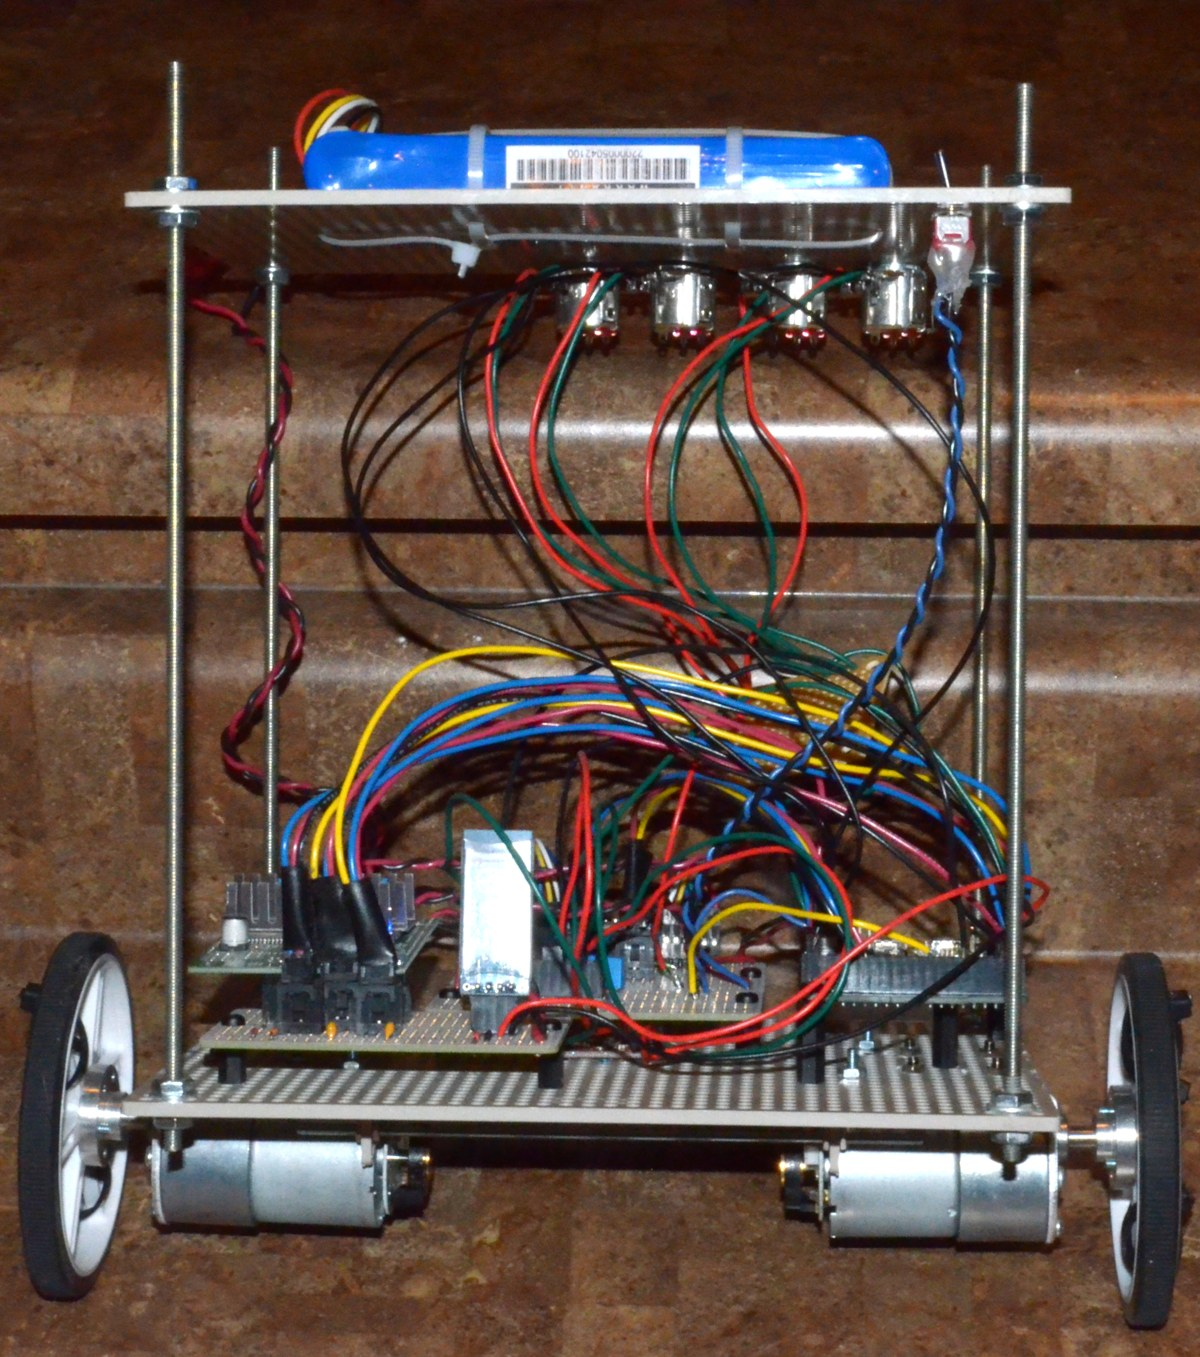
\includegraphics[width=0.45\textwidth]{twip_robot}
\caption{Two wheeled inverted pendulum robot.}
\label{fig:robot}
\end{figure}

\begin{table}[htbp]
\centering
\caption{TWIP robot physical parameters}
\label{tab:phys}
\begin{tabular}{lcc}
\toprule
Parameter & Value & Units \\
\midrule
Pendulum moment of inertia about the wheel axis, $I_p$ & 0.025\,$^a$ & \si{kg.m^2} \\
Wheel moment of inertia, $I_w$ & $1.441\times10^{-4}$\,$^b$ & \si{kg.m^2} \\
Distance to CG from wheel axis, $l$ & 0.075 & \si{m} \\
Mass of pendulum, $M_p$ & 1.432 & \si{kg} \\
Mass of wheels, $M_w$ & 0.1168 & \si{kg} \\
Wheel radius, $r$ & 0.045 & \si{m} \\
\bottomrule
\end{tabular}\\[2pt]
{\footnotesize $^a$ Computed with parallel-axis terms, i.e.\ about the wheel axis.
The equations of motion require the value about the center of gravity,
\SI{0.0169}{kg.m^2}; see Section~\ref{sec:simmodel}.\\
\rev{$^b$ The simulations, here and in the revision~7 programs, use the
uniform-disk value $M_wr^2/2=\SI{1.183e-4}{kg.m^2}$. The difference changes
$\beta$ of \eqref{eq:beta} by 1.4\%.}}
\end{table}

\rev{The moment of inertia and the CG offset are the two parameters least well
known on a build of this kind. Both are computed from a lumped-mass
idealization of the plates and components rather than measured. The gains that
balanced the hardware differ from the LQR gains computed from
Table~\ref{tab:phys}, but much of that difference is in the position and
velocity gains, whose sign the firmware's encoder frame affects
(Section~\ref{sec:gaintest}), so it does not measure the parameter error. The
recorded runs show the error nonetheless: at switch-on the tilt input gain is 8
to 26\% above the model (Section~\ref{sec:voltagetest}), and the accelerometer
points to an $I_p$ above the lumped-mass estimate
(Section~\ref{sec:momtest}). This is the motivation for the uncertainty
estimation problem rather than an incidental nuisance;
Appendix~\ref{app:validation} describes a pendulum-swing procedure for
measuring $I_p$ and $l$ directly.}

\section{ELECTRONIC DESIGN}

Electronics are a major component of any robot, and the two wheeled inverted
pendulum is no exception. The robot consists of a main computer, two motors,
various sensors, and power and communication devices.

\subsection{Computer}

The robot is controlled using an Arduino Due microcontroller board based on the
Atmel SAM3X8E ARM Cortex-M3, a 32-bit \SI{84}{MHz} CPU. The Due has
\SI{96}{kB} of onboard SRAM and \SI{512}{kB} of flash available for
programming. It provides 54 digital input/output channels, twelve of which can
be configured for pulse width modulation output, twelve analog inputs, and two
analog outputs, and supports serial communication over USB. The microcontroller
is programmed in C through the Arduino interface. The Arduino is a widely used
hobbyist platform and a broad range of integrated shields can be purchased to
work directly with it.

\rev{The Due is adequate for the control law but not generous. As documented in
Section~\ref{sec:difficulties}, serial transmission for telemetry dominated the
loop budget. Appendix~\ref{app:validation} recommends separating the
deterministic control path from the telemetry path so that the achievable loop
rate is set by the control computation rather than by the logging.}

\subsection{Motors}

Two Pololu \SI{12}{V} \SI{37}{mm} brushed DC motors drive the wheels. The
motors have a 30:1 gearbox and 64 counts-per-revolution integrated Hall effect
quadrature encoders measuring the position of the motor output shaft. The motors
are characterized by their free-run speed and current and their stall torque and
current; from these the torque constant $k_m$ and the back-EMF constant $k_e$
are obtained. The nominal terminal resistance is measured directly across the
output terminals at several shaft positions and averaged. The motor constants
are summarized in Table~\ref{tab:motor}.

Motor drive is provided by a Pololu Dual VNH5019 Motor Driver Arduino Shield.
The VNH5019 chip allows DC motor operation between \SI{5.5}{V} and \SI{24}{V} at
currents up to \SI{12}{A}, provides current sensing, and supports PWM operation
at ultrasonic frequencies up to \SI{20}{kHz} for quieter operation. The shield
is designed to work directly with the Arduino platform and a supplied library
provides straightforward control of two independent motors.

\begin{table}[htbp]
\centering
\caption{DC motor physical parameters}
\label{tab:motor}
\begin{tabular}{lcc}
\toprule
Parameter & Value & Units \\
\midrule
Free-run speed & 350 & RPM \\
Free-run current & 300 & mA \\
Stall torque & 110 & oz-in \\
Stall current & 5000 & mA \\
Torque motor constant, $k_m$ & 0.11541 & \si{N.m/A} \\
Back-EMF constant, $k_e$ & 0.307\,$^b$ & \si{V.s/rad} \\
Nominal resistance, $R$ & 2.5 & \si{\ohm} \\
\bottomrule
\end{tabular}\\[2pt]
{\footnotesize $^b$ From the free-run data above. Revision~7 used
\SI{0.00361}{V.s/rad}, which is inconsistent with those data by a factor of
about 85; see Section~\ref{sec:simmodel}.}
\end{table}

\subsection{Sensors}

Sensors are necessary in any robot in order to measure the state of the system,
and the state must be known in order to properly control it. In this system the
measurements are obtained from an integrated inertial measurement unit and from
Hall effect digital encoders integrated on each motor.

\subsubsection{Inertial measurement unit.}

Integrated System in Package (SiP) microchips are widely used in consumer
electronics owing to their small size and low production cost. The InvenSense
MPU-9150 is a low cost, low power SiP motion tracking device marketed for
equipment such as smartphones and tablets. It includes a three-axis gyroscope, a
three-axis accelerometer, a three-axis magnetometer, and an onboard Digital
Motion Processor (DMP) intended to offload algorithms from the main processor.
The SparkFun MPU-9150 breakout board is used here, which places the surface
mount device on a board with the communication pins available for direct
soldering. The DMP and the magnetometer were not used; only the direct
accelerometer and gyroscope readings are required to obtain the necessary
states.

The gyroscope has a 16-bit digital output with user-selectable ranges from
\SI{\pm250}{\degree/s} to \SI{\pm2000}{\degree/s}. The lowest range is selected
because it has the highest sensitivity, \SI{131}{LSB\per(\degree\per s)},
corresponding to a resolution of $1/131$ or approximately
\SI{0.00763}{\degree/s}. Noise is specified by two parameters: a total RMS noise
of \SI{0.06}{\degree/s} at a \SI{92}{Hz} rate, and a noise spectral density of
\SI{0.005}{\degree/s/\sqrt{Hz}} at \SI{10}{Hz}. These are characterized more
carefully by direct test in Section~\ref{sec:noise}. The specifications are
summarized in Table~\ref{tab:gyro}.

The accelerometer also has a 16-bit digital output, reporting in multiples of
gravity. Calibration was required to obtain a \SI{1}{g} reading at rest. At the
minimum range of \SI{\pm2}{g} the sensitivity is \SI{16384}{LSB\per g}, an exact
resolution of $1/16384$ or approximately \SI{61.0}{\micro g}. Noise is specified
as \SI{4}{mg} RMS at a \SI{100}{Hz} rate and a power spectral density of
\SI{400}{\micro g/\sqrt{Hz}} at \SI{10}{Hz}. The difference in the reference
rates between the two sensors necessitates a direct analysis of the noise from
the units actually used, so that the simulation is representative. The
accelerometer specifications are summarized in Table~\ref{tab:accel}.

\begin{table}[htbp]
\centering
\caption{Gyroscope specifications}
\label{tab:gyro}
\begin{tabular}{lcc}
\toprule
Parameter & Value & Units \\
\midrule
Range & $\pm250$ & \si{\degree/s} \\
Sensitivity & 131 & LSB/(\si{\degree/s}) \\
Resolution & 0.00763 & \si{\degree/s} \\
Total RMS noise & 0.06 & \si{\degree/s} RMS \\
Power spectral density & 0.005 & \si{\degree/s/\sqrt{Hz}} \\
\bottomrule
\end{tabular}
\end{table}

\begin{table}[htbp]
\centering
\caption{Accelerometer specifications}
\label{tab:accel}
\begin{tabular}{lcc}
\toprule
Parameter & Value & Units \\
\midrule
Range & $\pm2$ & \si{g} \\
Sensitivity & 16384 & LSB/\si{g} \\
Resolution & 61.0 & \si{\micro g} \\
Total RMS noise & 4 & \si{mg} RMS \\
Power spectral density & 400 & \si{\micro g/\sqrt{Hz}} \\
\bottomrule
\end{tabular}
\end{table}

\subsubsection{Digital encoders.}

Each Pololu metal DC motor has an integrated Hall effect quadrature encoder
measuring the relative position of the motor output shaft. The shaft carries a
magnetic disk with 16 magnetic divisions, and two Hall effect sensors detect the
changing field as the shaft rotates. Counting both the rising and falling edges
of both signals gives a total resolution of 64 counts per revolution of the
motor output shaft. \rev{The two signals are a quarter cycle (\SI{90}{\degree})
apart, in quadrature, which is the origin of the term and what allows the
direction of rotation to be decoded.} In
combination with the 30:1 gearbox, the gearbox output has a measurable
resolution of 1920 counts per revolution. With \SI{90}{mm} diameter wheels the
encoder measures discrete steps of \SI{1.47e-4}{m}.

\rev{The encoders are mounted on the motor shaft, ahead of the gearbox. Gear
backlash is therefore invisible to the encoder: the measured shaft angle
advances while the wheel does not. This is a structural measurement limitation,
not a resolution limitation, and it cannot be removed by increasing the sample
rate. Appendix~\ref{app:validation} discusses load-side encoding as the remedy.}

\subsection{Miscellaneous Electronics}

Four potentiometers are connected to the Arduino Due to allow easy adjustment of
parameters, in this case the controller gains, and a switch is used to enable
and disable the controller. Miscellaneous level-shifting electronics are
included to permit communication with the Due, as is an HC-05 Bluetooth module
for wireless transmission of serial output data. The robot is powered by a
single high-discharge \SI{11.1}{V} 20C lithium polymer battery.

\section{PROGRAMMING}

On initialization the various pins and connections are configured, enabling
communication between the sensors, switches, Bluetooth module, and the
microcontroller. The motor controller is initialized and the IMU is enabled. On
initialization of the IMU the constant bias is removed from the sensor
measurements by averaging a run of samples taken with the robot stationary.

\subsection{Measurements}
\label{sec:measurements}

The accelerometer measures the specific force vector, which at rest is the
gravitational field vector expressed in body axes. Writing the measured vector
as $\mathbf{G}_p=[a_x\ a_y\ a_z]^T$ and relating it to the gravitational field
through a rotation sequence in roll $\varphi$ and pitch $\vartheta_p$
\cite{kuipers1999quaternions},
\begin{equation}\label{eq:gravvec}
\frac{\mathbf{G}_p}{\norm{\mathbf{G}_p}}
=\frac{1}{\sqrt{a_x^2+a_y^2+a_z^2}}
\begin{bmatrix}a_x\\a_y\\a_z\end{bmatrix}
=\begin{bmatrix}
-\sin\vartheta_p\\
\cos\vartheta_p\sin\varphi\\
\cos\vartheta_p\cos\varphi
\end{bmatrix},
\end{equation}
which can be solved for the roll and pitch angles,
\begin{equation}\label{eq:rollpitch}
\varphi=\tan^{-1}\!\left(\frac{a_y}{a_z}\right),
\qquad
\vartheta_p=\tan^{-1}\!\left(\frac{-a_x}{\sqrt{a_y^2+a_z^2}}\right).
\end{equation}

The relationship in \eqref{eq:rollpitch} is only one way to compute the pitch
from the accelerometer. Rotation matrices do not commute, but as only the pitch
angle is of concern a different rotation sequence may be used to obtain the same
pitch measurement. Computation on the microcontroller must be minimized wherever
possible, so by using the rotation sequence $R_{yxz}$ in the same manner an
easier relationship for the tilt angle is obtained,
\begin{equation}\label{eq:tiltaccel}
\theta_a=\tan^{-1}\!\left(\frac{a_x}{a_z}\right).
\end{equation}

This calculation assumes two things: that the initial orientation of the
accelerometer is aligned with the gravitational field vector along the $z$ axis,
and that there are no external accelerations. The second clearly fails when the
robot is moving, so filtering of this measurement is necessary. A complementary
filter \cite{higgins1975comparison} is used. The same task could be performed
by a Kalman filter, but the computational limitations of the microcontroller
make the complementary filter the appropriate choice. The filter combines the
accelerometer and gyroscope measurements to obtain a more accurate angle
estimate using a simplified high-pass and low-pass pair. The form implemented on
the robot is
\begin{equation}\label{eq:compfilter}
\theta_{k+1}=\lambda_c\bigl(\theta_k+g_y\Delta t\bigr)+\bigl(1-\lambda_c\bigr)\theta_a ,
\end{equation}
where $\lambda_c$ is a design parameter set to $0.99$, $g_y$ is the $y$-axis
gyroscope reading, $\theta_a$ is the accelerometer tilt angle from
\eqref{eq:tiltaccel}, and $\theta_k$ is the filter angle estimate. The
complementary filter is simple to implement and well suited to an
implementation where computation is limited.

The tilt angle is the only measurement that must be pre-filtered before the
DMSO or the Kalman filter are used to estimate the full state. The gyroscope
measurements are used directly for the tilt rate. The motor encoder outputs are
processed using hardware interrupts: each time a Hall effect sensor signal
changes state the interrupt fires and increments or decrements the encoder
position. Velocity is obtained by differencing the position readings.

\rev{\begin{remark}[The pre-filter is part of the measurement model]
Equation \eqref{eq:compfilter} is a dynamic element placed between the sensors
and the estimator, so the quantity presented to the DMSO as $y_k$ is not a raw
measurement but a filtered one with its own lag and its own error
characteristics. Two consequences follow. First, the measurement noise
covariance used by the Kalman filter baseline must describe the complementary
filter output, not the accelerometer. Second, the comparison reported in
Section~\ref{sec:implresults}, in which the complementary filter outperforms
both model-based estimators fed raw accelerometer tilt, is a statement about
this pre-filtering step rather than about the estimators.
\end{remark}}

\section{DIFFICULTIES}
\label{sec:difficulties}

During assembly and programming many difficulties were encountered. Initially
the motors were a substantial problem and were eventually replaced. The original
motors were \SI{6}{V} DC units with lower torque output and an enormous deadzone
nonlinearity, giving a correspondingly small range of controllable output.
Simulation studies showed that the best achievable behavior with those motors
was a large stable oscillation, and sensor noise made even that unachievable.
It was during this period that the potentiometers were added, so that controller
gains could be adjusted quickly without reprogramming the microcontroller.

The motors were replaced with larger \SI{12}{V} units that do not have the same
large deadzone and allow a wider output range for control. This created a
problem with the plastic mounting plates, which twisted under the additional
weight until stiffening rods were added to the underside. It also exposed an
initial design flaw: plastic rods were used to separate the two mounting plates,
and the resulting flexure allowed vibrations to contaminate the sensor
measurements. Steel threaded rods were substituted and stiffened the structure
satisfactorily.

The robot is limited in available computation, so computations were minimized
wherever possible. Serial output proved to be one of the largest consumers of
computational effort. Serial data is essential for evaluating performance, so
its content had to be selected carefully and limited in order to keep the loop
time acceptable. The minimum loop execution time obtained was \SI{0.01}{s}.

The LQR gains had to be modified from the values computed from the measured
parameters of the robot, which \rev{revision~7 took as evidence of}
inaccurately measured parameters. The model is also not entirely accurate to the true system: the
pendulum is modeled as a point mass attached by a thin beam to the motor axis,
whereas the mounting plates create more complex interactions than this.
\rev{Once the gains were retuned the robot balanced, for up to \SI{21}{s},
although none of the recorded gain sets is linearly stable on any candidate
model (Table~\ref{tab:gaintest}).}
\rev{The logs point to a more specific cause (Section~\ref{sec:gaintest}). The
switch-on transients indicate that the firmware's encoder position is mirrored
relative to the model. In that frame, position and velocity gains entered with
the signs of the LQR design act with the opposite sign on the robot, and the
position and velocity potentiometers, which the firmware maps to $[-15,0]$,
could not set the signs the design requires. Both v9 runs balanced on the tilt
gains, with the base held within a few millimeters; in the two v8 runs the base
drove away until the robot was switched off (test~1) or until a chatter ended
the run (test~2). In closed-loop simulation the corrected model reproduces the
v9 runs in that frame only if the floor resisted rolling by a few percent of
the weight, so the frame is not yet confirmed. Either way, the modification of
the gains is not evidence of parameter error alone.}

\rev{\begin{remark}[These are the case for the work]
Three of the observations above are the empirical case for
Chapters~\ref{ch:dmso} and~\ref{ch:control} rather than incidental setbacks. The
parameters are uncertain, which motivates online uncertainty estimation. The
actuator is nonlinear in a way the linear model does not capture, which
motivates the unmatched uncertainty formulation. The available computation
constrains the achievable sample rate, which is an implementation constraint
treated as a design variable in Appendix~\ref{app:validation} rather than as a
fixed property of the platform.
\end{remark}}

\chapter{THE BALANCING ROBOT MODEL}
\label{ch:model}

\section{MODEL OF A DIRECT CURRENT MOTOR}
\label{sec:motor}

The armature circuit of a brushed DC motor with terminal voltage $V_a$,
resistance $R$, inductance $L$, and back-EMF constant $k_e$ obeys Kirchhoff's
voltage law \cite{desilva2004mechatronics},
\begin{equation}\label{eq:circuit}
L\frac{\dd i}{\dd t}+Ri+k_e\omega=V_a ,
\end{equation}
where $i$ is the armature current and $\omega=\dot\vartheta$ the shaft rate.
Rearranging,
\begin{equation}\label{eq:circuit2}
\frac{\dd i}{\dd t}=\frac{V_a}{L}-\frac{R}{L}i-\frac{k_e}{L}\omega .
\end{equation}
The electromagnetic torque developed is proportional to the current,
\begin{equation}\label{eq:torque}
\tau_m=k_mi ,
\end{equation}
and the viscous friction torque is proportional to the shaft rate,
\begin{equation}\label{eq:friction}
\tau_f=k_f\omega .
\end{equation}
Applying Newton's second law and summing moments about the motor output shaft
against an applied load torque $\tau_a$ and load inertia $I_m$,
\begin{equation}\label{eq:shaft}
I_m\dot\omega=\tau_m-\tau_f-\tau_a .
\end{equation}
Substituting \eqref{eq:torque} and \eqref{eq:friction} into \eqref{eq:shaft} and
rearranging gives the second equation of motion,
\begin{equation}\label{eq:shaft2}
\frac{\dd\omega}{\dd t}=\frac{k_m}{I_m}i-\frac{k_f}{I_m}\omega-\frac{\tau_a}{I_m} .
\end{equation}

Equations \eqref{eq:circuit2} and \eqref{eq:shaft2} describe the fundamental
behavior of a DC motor as a pair of first-order differential equations relating
circuit current, motor speed, and applied torque. For a balancing robot a
simplified model provides acceptable performance. Assuming the motor inductance
$L$ and the friction coefficient $k_f$ are negligible,
\begin{equation}\label{eq:isimple}
i=\frac{V_a}{R}-\frac{k_e}{R}\omega ,
\end{equation}
and
\begin{equation}\label{eq:wsimple}
\frac{\dd\omega}{\dd t}=\frac{k_m}{I_m}i-\frac{\tau_a}{I_m} .
\end{equation}
Substituting \eqref{eq:isimple} into \eqref{eq:wsimple} gives a model that does
not include the circuit current,
\begin{equation}\label{eq:motor}
\frac{\dd\omega}{\dd t}
=-\frac{k_mk_e}{I_mR}\omega+\frac{k_m}{I_mR}V_a-\frac{\tau_a}{I_m} .
\end{equation}
This elimination is desirable: the current is not directly commandable on the
physical system and would add a state with no observable benefit. Neglecting the
inductance amounts to assuming the current reaches steady state immediately
relative to the motor speed, which is justified because the electrical time
constant $L/R$ is orders of magnitude shorter than the mechanical one. In
state-space form,
\begin{equation}\label{eq:motorss}
\frac{\dd}{\dd t}
\begin{bmatrix}\vartheta\\\omega\end{bmatrix}
=\begin{bmatrix}
0 & 1\\[4pt]
0 & -\dfrac{k_mk_e}{I_mR}
\end{bmatrix}
\begin{bmatrix}\vartheta\\\omega\end{bmatrix}
+\begin{bmatrix}
0 & 0\\[4pt]
\dfrac{k_m}{I_mR} & -\dfrac{1}{I_m}
\end{bmatrix}
\begin{bmatrix}V_a\\\tau_a\end{bmatrix}.
\end{equation}

\section{TWO WHEELED INVERTED PENDULUM DYNAMIC MODEL}
\label{sec:twipmodel}

The TWIP shares many similarities with the pendulum-on-a-cart problem. The
motion is comparable but the dynamics are more involved. The analysis begins
with the two wheels, the pendulum is analyzed separately, and the two sets of
equations are combined by eliminating the interface reactions, yielding two
dynamic equations describing the motion of the system.

\subsection{Wheel Dynamics}

The free-body diagram of the left wheel is shown in Figure~\ref{fig:fbdwheel}.
The reaction forces between the wheel and the pendulum are $P_L$ and $H_L$, the
torque applied to the wheel by the DC motor is $C_L$, and the friction force
between the ground and the wheel is $H_{fL}$. The equations for the left and
right wheels are completely analogous, so only the left wheel is analyzed. The
wheels are assumed to remain in ground contact at all times with no slip.

\begin{figure}[htbp]
\centering
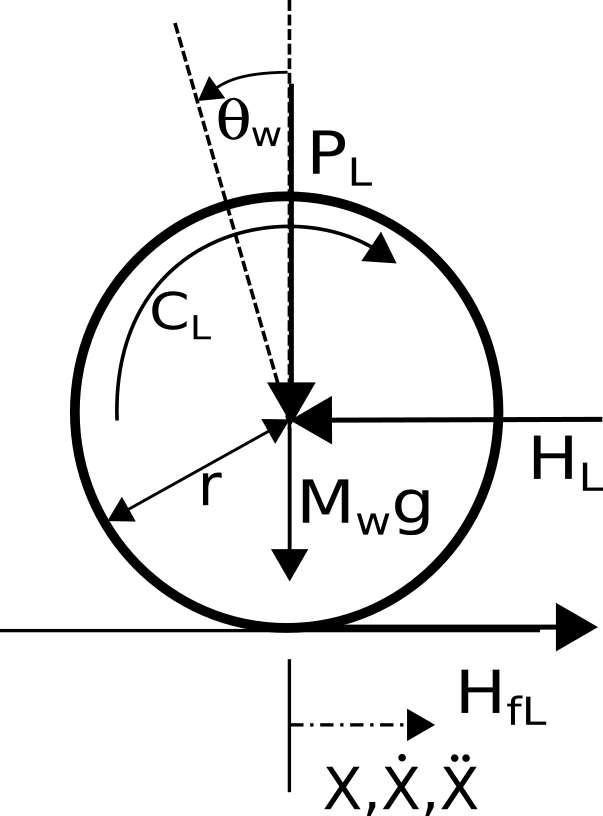
\includegraphics[width=0.45\textwidth]{fbd_wheel}
\caption{Left wheel free body diagram.}
\label{fig:fbdwheel}
\end{figure}

Summing forces in the $x$ direction,
\begin{equation}\label{eq:wheelx}
M_w\ddot x=H_{fL}-H_L .
\end{equation}
Summing moments about the center of the wheel,
\begin{equation}\label{eq:wheelm}
I_w\ddot\theta_w=C_L-H_{fL}r ,
\end{equation}
where $I_w$ is the wheel moment of inertia and $\ddot\theta_w$ the wheel angular
acceleration. Starting from the motor shaft equation \eqref{eq:shaft} and
substituting \eqref{eq:isimple}, the motor torque delivered to either wheel is
\begin{equation}\label{eq:CL}
C_L=C_R=\tau_m=-\frac{k_mk_e}{R}\dot\theta_w+\frac{k_m}{R}V_a .
\end{equation}
\rev{In \eqref{eq:CL}, $\dot\theta_w$ must be read as the wheel rate relative to
the motor stator, which is fixed to the pendulum body. The development below
follows revision~7 in substituting the absolute rate $\dot x/r$, which drops a
tilt-rate term; the correction used for the results is given in
Section~\ref{sec:simmodel}.}
Using \eqref{eq:CL} in \eqref{eq:wheelm} and rearranging gives the friction
reaction force,
\begin{equation}\label{eq:HfL}
H_{fL}=-\frac{k_mk_e}{Rr}\dot\theta_w+\frac{k_m}{Rr}V_a
-\frac{I_w}{r}\ddot\theta_w .
\end{equation}
Substituting \eqref{eq:HfL} into \eqref{eq:wheelx} gives the equation of motion
for the left wheel,
\begin{equation}\label{eq:wheelL}
M_w\ddot x=-\frac{k_mk_e}{Rr}\dot\theta_w+\frac{k_m}{Rr}V
-\frac{I_w}{r}\ddot\theta_w-H_L ,
\end{equation}
and an identical development for the right wheel gives
\begin{equation}\label{eq:wheelR}
M_w\ddot x=-\frac{k_mk_e}{Rr}\dot\theta_w+\frac{k_m}{Rr}V
-\frac{I_w}{r}\ddot\theta_w-H_R .
\end{equation}

The no-slip assumption provides the transformation between rotational and
linear motion,
\begin{equation}\label{eq:noslip}
\ddot\theta_w=\frac{\ddot x}{r},\qquad \dot\theta_w=\frac{\dot x}{r} .
\end{equation}
Applying \eqref{eq:noslip} to \eqref{eq:wheelL} and \eqref{eq:wheelR},
\begin{align}
M_w\ddot x&=-\frac{k_mk_e}{Rr^2}\dot x+\frac{k_m}{Rr}V
-\frac{I_w}{r^2}\ddot x-H_L ,\label{eq:wheelL2}\\[4pt]
M_w\ddot x&=-\frac{k_mk_e}{Rr^2}\dot x+\frac{k_m}{Rr}V
-\frac{I_w}{r^2}\ddot x-H_R .\label{eq:wheelR2}
\end{align}
Adding \eqref{eq:wheelL2} and \eqref{eq:wheelR2} gives the equation of motion
for the combined wheel system,
\begin{equation}\label{eq:wheelcomb}
2\left(M_w+\frac{I_w}{r^2}\right)\ddot x
=-\frac{2k_mk_e}{Rr^2}\dot x+\frac{2k_m}{Rr}V-\bigl(H_L+H_R\bigr).
\end{equation}

\subsection{Pendulum Dynamics}

Figure~\ref{fig:fbdpend} shows the free-body diagram of the inverted pendulum.
Two reference frames are used: an inertial frame attached to the base of the
pendulum, and a translating frame at the center of gravity. Here $l$ is the
distance from the base to the center of gravity; $\alpha_p$, $\omega_p$, and
$\theta$ are the angular acceleration, angular velocity, and angular position of
the pendulum; $x,\dot x,\ddot x$ are the position, velocity, and acceleration of
the pendulum base; and $x_p,\dot x_p,\ddot x_p$ those of the center of gravity.

\begin{figure}[htbp]
\centering
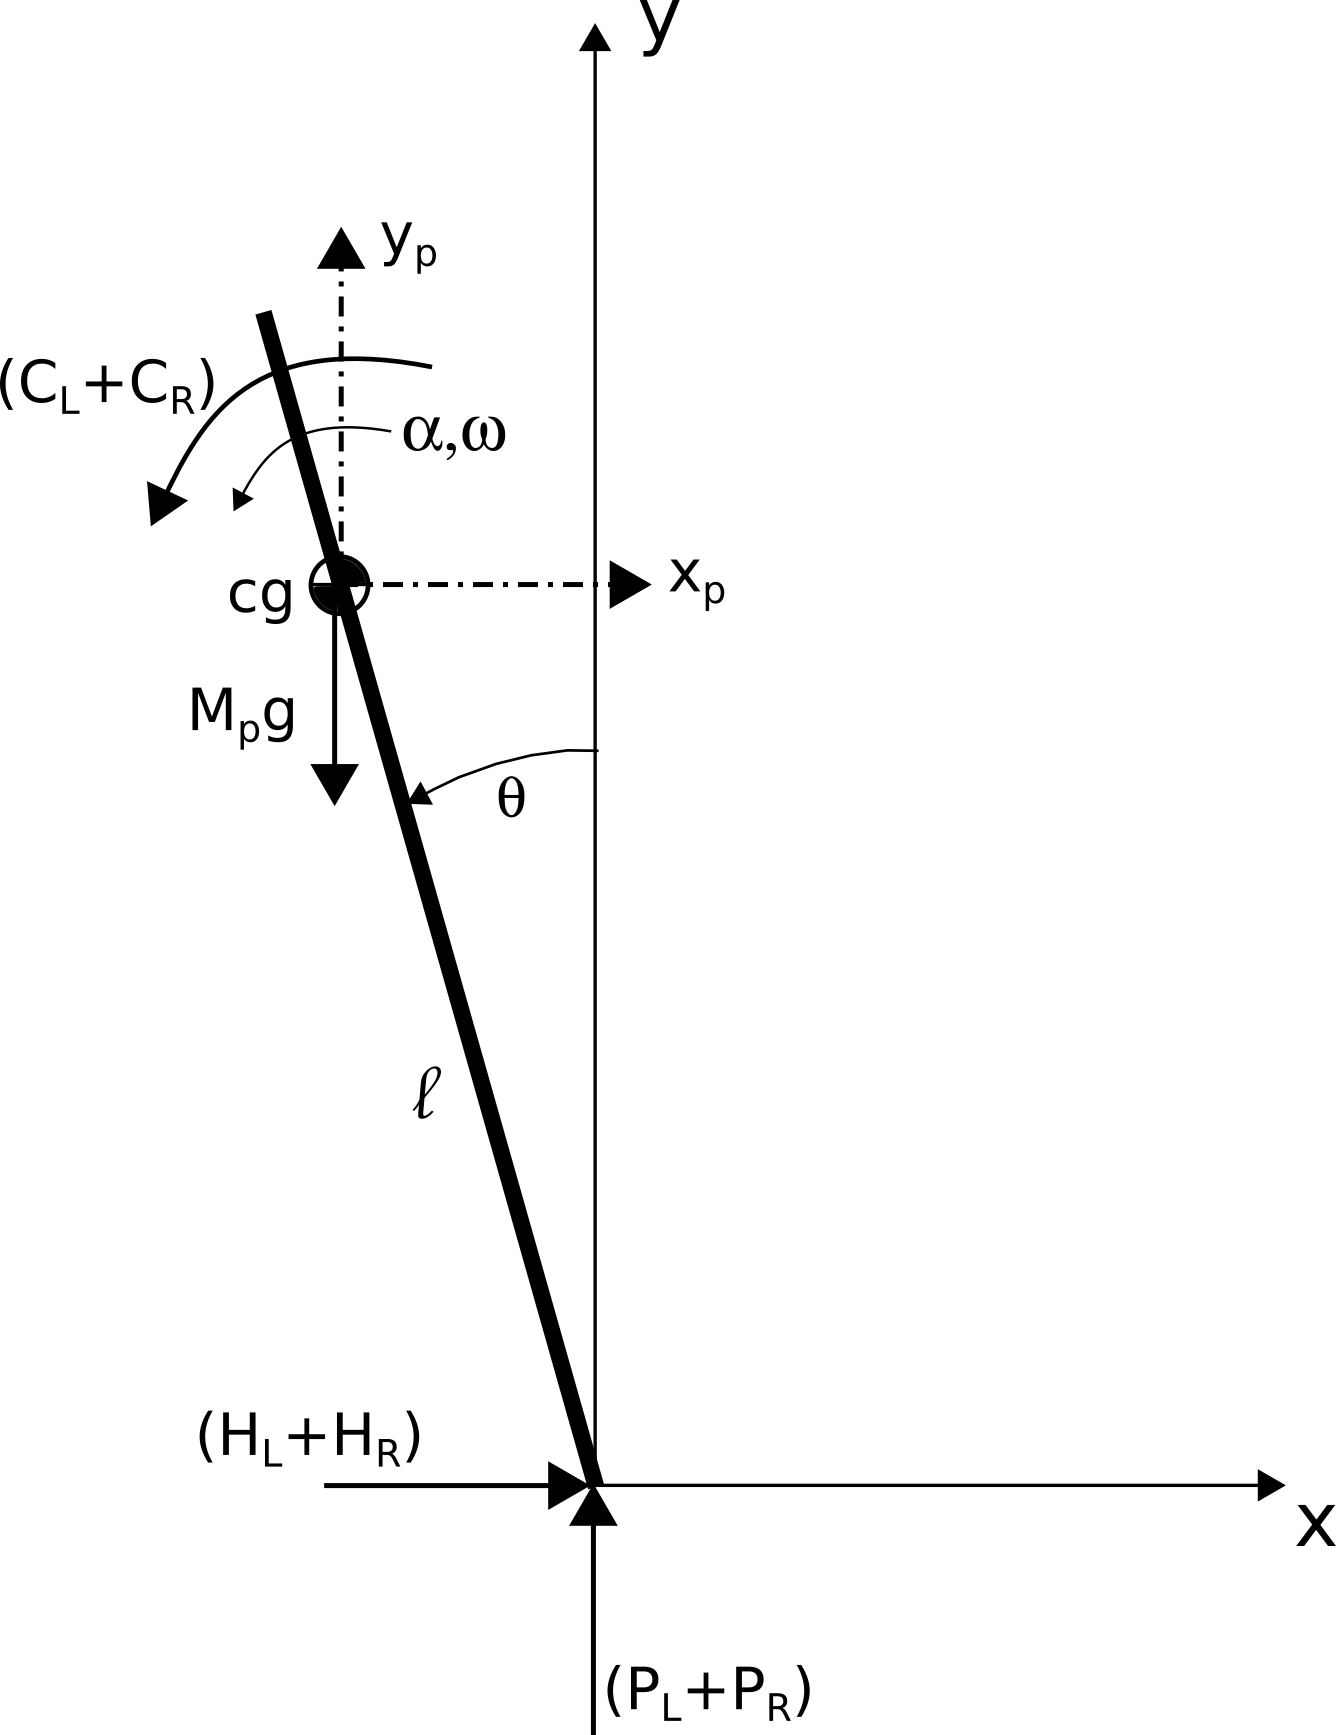
\includegraphics[width=0.45\textwidth]{fbd_pendulum}
\caption{Inverted pendulum free body diagram.}
\label{fig:fbdpend}
\end{figure}

Summing forces in the $x_p$ direction,
\begin{equation}\label{eq:pendx}
\sum F_{xp}=H_L+H_R=M_p\ddot x_p ,
\end{equation}
and in the $y_p$ direction,
\begin{equation}\label{eq:pendy}
\sum F_{yp}=P_L+P_R-M_pg=M_p\ddot y_p .
\end{equation}

The acceleration of a point in a translating frame follows from relative motion
analysis \cite{hibbeler2010dynamics}. The acceleration of the pendulum center of
gravity, denoted $\mathbf{a}_B$, is
\begin{equation}\label{eq:relmotion}
\mathbf{a}_B=\mathbf{a}_A
+\bm{\alpha}_p\times\mathbf{r}_{B/A}
+\bm{\omega}_p\times\bigl(\bm{\omega}_p\times\mathbf{r}_{B/A}\bigr),
\end{equation}
with
\begin{align}
\mathbf{a}_B&=\ddot x_p\hat\imath+\ddot y_p\hat\jmath ,\label{eq:aB}\\
\mathbf{r}_{B/A}&=l\sin\theta\,\hat\imath-l\cos\theta\,\hat\jmath ,\label{eq:rBA}\\
\bm{\omega}_p&=\dot\theta\,\hat k ,\label{eq:omegap}\\
\bm{\alpha}_p&=\ddot\theta\,\hat k ,\label{eq:alphap}\\
\mathbf{a}_A&=\ddot x\,\hat\imath .\label{eq:aA}
\end{align}
Using \eqref{eq:rBA}--\eqref{eq:aA} in \eqref{eq:relmotion},
\begin{equation}\label{eq:aBfull}
\mathbf{a}_B=\Bigl(\ddot x+\ddot\theta l\cos\theta-\dot\theta^2l\sin\theta\Bigr)\hat\imath
+\Bigl(\ddot\theta l\sin\theta+\dot\theta^2l\cos\theta\Bigr)\hat\jmath .
\end{equation}
Substituting \eqref{eq:aBfull} into \eqref{eq:pendx} and \eqref{eq:pendy},
\begin{align}
H_L+H_R&=M_p\Bigl(\ddot x+\ddot\theta l\cos\theta-\dot\theta^2l\sin\theta\Bigr),
\label{eq:Hsum}\\[4pt]
P_L+P_R&=M_pg+M_p\Bigl(\ddot\theta l\sin\theta+\dot\theta^2l\cos\theta\Bigr).
\label{eq:Psum}
\end{align}

Summing moments about the pendulum center of gravity, with the clockwise
direction taken as positive,
\begin{equation}\label{eq:pendm}
\sum M=-\bigl(C_L+C_R\bigr)-\bigl(H_L+H_R\bigr)l\cos\theta
-\bigl(P_L+P_R\bigr)l\sin\theta=I_p\ddot\theta .
\end{equation}

\subsection{Combined Equations of Motion}

Combining \eqref{eq:CL}, \eqref{eq:Hsum}, \eqref{eq:Psum}, and \eqref{eq:pendm},
\begin{equation}\label{eq:combined}
\begin{aligned}
-\left(-\frac{2k_mk_e}{R}\dot\theta_w+\frac{2k_m}{R}V_a\right)
&-\Bigl(M_p\bigl(\ddot x+\ddot\theta l\cos\theta-\dot\theta^2l\sin\theta\bigr)\Bigr)l\cos\theta\\
&-\Bigl(M_pg+M_p\bigl(\ddot\theta l\sin\theta+\dot\theta^2l\cos\theta\bigr)\Bigr)l\sin\theta
=I_p\ddot\theta .
\end{aligned}
\end{equation}
Cancelling terms, rearranging, and applying the identity
$\sin^2\theta+\cos^2\theta=1$ gives the first nonlinear equation of motion,
\begin{equation}\label{eq:nl1}
\bigl(I_p+M_pl^2\bigr)\ddot\theta
-\frac{2k_mk_e}{Rr}\dot x
+\frac{2k_m}{R}V
+M_pgl\sin\theta
=-M_pl\ddot x\cos\theta .
\end{equation}
Using \eqref{eq:Hsum} to remove the body forces from \eqref{eq:wheelcomb} gives
the second nonlinear equation of motion,
\begin{equation}\label{eq:nl2}
\frac{2k_m}{Rr}V=\left(2M_w+\frac{2I_w}{r^2}+M_p\right)\ddot x
+\frac{2k_mk_e}{Rr^2}\dot x
+M_pl\ddot\theta\cos\theta
-M_pl\dot\theta^2\sin\theta .
\end{equation}

Equations \eqref{eq:nl1} and \eqref{eq:nl2} describe the full nonlinear motion
of the two-wheeled inverted pendulum.

\subsection{Linearization}

In the convention of Figure~\ref{fig:fbdpend}, $\theta=\pi$ is the upright
vertical configuration. A set of linearized equations is obtained by writing
$\theta=\pi+\phi$, where $\phi$ is a small angle from the vertical. The
small-angle assumptions are
\begin{equation}\label{eq:smallangle}
\cos\theta=-1,\qquad \sin\theta=-\phi,
\end{equation}
together with the assumption that the squared angular rate is small,
\begin{equation}\label{eq:smallrate}
\dot\theta^2=0 .
\end{equation}
Applying \eqref{eq:smallangle} and \eqref{eq:smallrate} to \eqref{eq:nl1} and
\eqref{eq:nl2} yields the linearized equations of motion,
\begin{align}
\bigl(I_p+M_pl^2\bigr)\ddot\phi-\frac{2k_mk_e}{Rr}\dot x
+\frac{2k_m}{R}V-M_pgl\phi&=M_pl\ddot x ,\label{eq:lin1}\\[4pt]
\frac{2k_m}{Rr}V=\left(2M_w+\frac{2I_w}{r^2}+M_p\right)\ddot x
+\frac{2k_mk_e}{Rr^2}\dot x-M_pl\ddot\phi&. \label{eq:lin2}
\end{align}

\rev{\begin{remark}[Sign of the gravity term]\label{rem:gravsign}
Rearranging \eqref{eq:lin1} gives
$\bigl(I_p+M_pl^2\bigr)\ddot\phi=M_pgl\phi+\cdots$, so the gravitational term
enters with positive sign and is destabilizing. This is the expected signature
of an upright linearization and confirms the convention: $\phi$ is the
displacement from the \emph{unstable} equilibrium, not from the hanging one. It
is also consistent with \eqref{eq:linss}, whose $(2,3)$ and $(4,3)$ entries are
both positive. The description of $\theta=\pi$ in revision~7 as the
``statically stable vertical point'' is a mislabeling; the corrected reading is
given in Section~\ref{sec:modelsim}.
\end{remark}}

Rearranging \eqref{eq:lin1} and \eqref{eq:lin2} into state-space form
$\dot{\mathbf{x}}=\mathcal{A}\mathbf{x}+\mathcal{B}V$ with
$\mathbf{x}=\begin{bmatrix}x&\dot x&\phi&\dot\phi\end{bmatrix}^T$ gives
\begin{equation}\label{eq:linss}
\mathcal{A}=
\begin{bmatrix}
0 & 1 & 0 & 0\\[4pt]
0 & \dfrac{2k_mk_e\bigl(M_plr-I_p-M_pl^2\bigr)}{Rr^2\alpha}
  & \dfrac{M_p^2gl^2}{\alpha} & 0\\[8pt]
0 & 0 & 0 & 1\\[4pt]
0 & \dfrac{2k_mk_e\bigl(r\beta-M_pl\bigr)}{Rr^2\alpha}
  & \dfrac{M_pgl\beta}{\alpha} & 0
\end{bmatrix},
\qquad
\mathcal{B}=
\begin{bmatrix}
0\\[4pt]
\dfrac{2k_m\bigl(I_p+M_pl^2-M_plr\bigr)}{Rr\alpha}\\[8pt]
0\\[4pt]
\dfrac{2k_m\bigl(M_pl-r\beta\bigr)}{Rr\alpha}
\end{bmatrix},
\end{equation}
where
\begin{equation}\label{eq:beta}
\beta:=2M_w+\frac{2I_w}{r^2}+M_p
\end{equation}
and
\begin{equation}\label{eq:alphadef}
\alpha:=I_p\beta+2M_pl^2\left(M_w+\frac{I_w}{r^2}\right).
\end{equation}

For the development in Chapter~\ref{ch:control} it is convenient to name the
entries of \eqref{eq:linss} directly. Writing $x_1=x$, $x_2=\dot x$, $x_3=\phi$,
$x_4=\dot\phi$, $u=V$, and appending the unmodeled and parametric uncertainty as
$d_1$ and $d_2$,
\begin{equation}\label{eq:plantform}
\begin{aligned}
\dot x_1&=x_2,\\
\dot x_2&=A_1x_2+A_2x_3+B_1u+d_1(\mathbf{x}),\\
\dot x_3&=x_4,\\
\dot x_4&=A_3x_2+A_4x_3+B_2u+d_2(\mathbf{x}),
\end{aligned}
\end{equation}
with $A_1,\dots,A_4,B_1,B_2$ read off from \eqref{eq:linss}. Note that
$A_4=0$ in the nominal model, since the tilt rate does not appear in the tilt
acceleration once friction is neglected; it is retained symbolically because the
uncertainty $d_2$ generally reintroduces such a dependence.

\rev{\begin{remark}[Structural consequences]
Two features of \eqref{eq:plantform} drive everything that follows. First,
$B_1$ and $B_2$ are both nonzero and the input is scalar, so the system is
underactuated and no choice of $u$ cancels both $d_1$ and $d_2$: the uncertainty
is unmatched. Second, $A_2\neq0$, so the tilt state enters the translational
acceleration directly. This is what makes $x_3$ usable as a virtual control for
the position subsystem, and it is also the term that couples the two error
subsystems in the backstepping design. It must be retained; see
Section~\ref{sec:cffb}.
\end{remark}}

\section{MODEL SIMULATION STUDY}
\label{sec:modelsim}

The model should be checked for accuracy and for the expected motion of an
inverted pendulum. This is done by examining the uncontrolled motion of the
nonlinear equations \eqref{eq:nl1}--\eqref{eq:nl2}; any consistent set of
parameter values may be used.

\rev{Two equilibria exist. In the convention of \eqref{eq:smallangle},
$\theta=\pi$ is the upright configuration and $\theta=0$ the hanging one. The
hanging point is statically stable; the upright point is an equilibrium but is
unstable, as Remark~\ref{rem:gravsign} establishes, so a trajectory started
exactly there with zero rate remains there while any perturbation grows.
Revision~7 described the two in the opposite sense. The numerical tests below
are unchanged; only their interpretation is corrected.}

Starting from $\theta=\SI{180}{\degree}$ with zero initial rate, the system
remains at that point, as shown in Figure~\ref{fig:stab180}. \rev{This confirms
that $\theta=\pi$ is an equilibrium of the implemented equations. It is not
evidence of stability, and a small perturbation about this point diverges, which
is the behavior required of an inverted pendulum and the reason active control
is needed at all.}

Starting from $\theta=\SI{10}{\degree}$, the system is expected to oscillate
about the hanging equilibrium $\theta=0$. With no friction modeled, the motor
back-EMF term supplies a damping-like effect and the oscillations decay.
Examining the free-body diagram in Figure~\ref{fig:fbdpend}, a small positive
angle should cause the body to move initially in the positive direction as the
tilt returns toward zero. Figure~\ref{fig:stab10} shows this behavior.
\rev{With the corrected back-EMF constant of Section~\ref{sec:simmodel}, the
damping is strong and the oscillation decays within about five periods. The
translational position does not return to zero; after the initial positive
excursion the base settles about \SI{8}{mm} behind its starting point, the
net effect of the asymmetric damping over the swings. The figures show the
corrected model used for the results of Chapter~\ref{ch:results}.} These checks
establish that the nonlinear equations of motion behave as expected and can be
relied upon.

\begin{figure}[htbp]
\centering
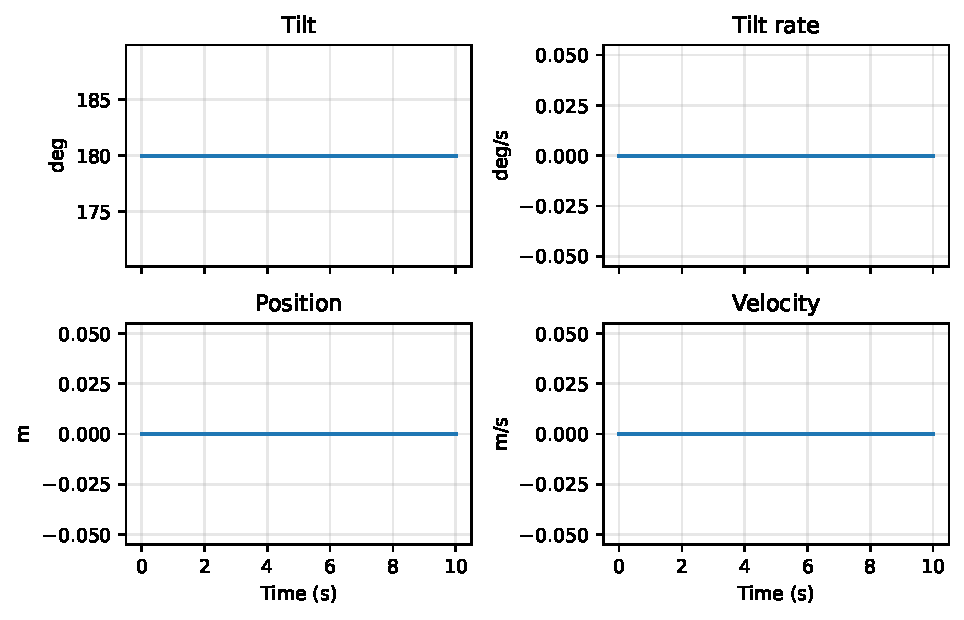
\includegraphics[width=0.8\textwidth]{stability_180}
\caption{Uncontrolled response from $\theta=\SI{180}{\degree}$.}
\label{fig:stab180}
\end{figure}

\begin{figure}[htbp]
\centering
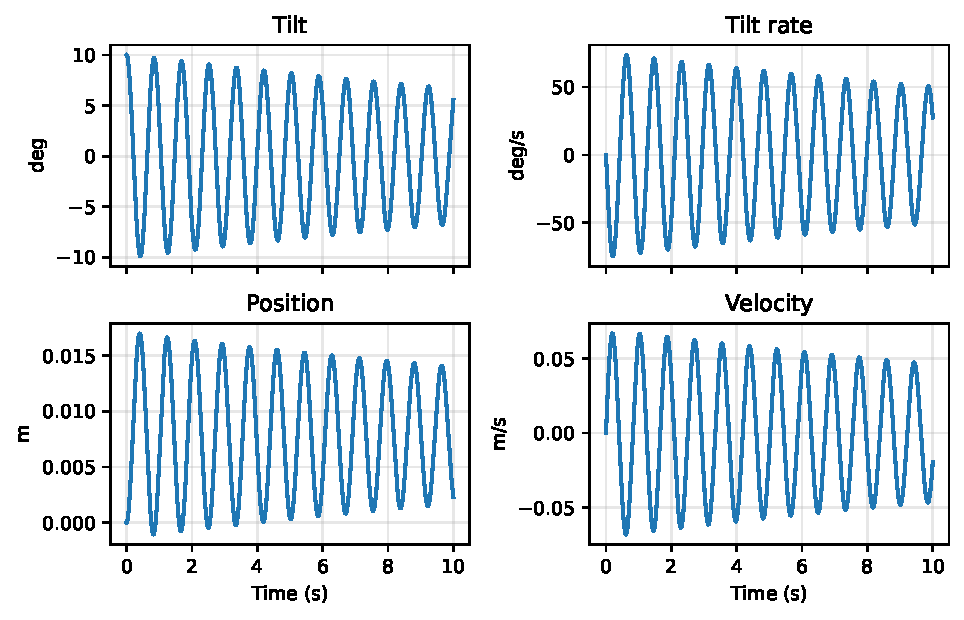
\includegraphics[width=0.8\textwidth]{stability_10}
\caption{Uncontrolled response from $\theta=\SI{10}{\degree}$.}
\label{fig:stab10}
\end{figure}

\chapter{CONTROL DESIGN}
\label{ch:control}

The TWIP is unstable and must be actively controlled. Linear control is
effective near the upright equilibrium when the parameters are accurately known,
so a linear quadratic regulator is used as the nominal control. An additive
signal is then formulated to compensate for the unmatched uncertainties
appearing in the two acceleration equations of \eqref{eq:plantform}.

\section{LQR CONTROL DESIGN}
\label{sec:lqr}

Because the controller is implemented digitally, the discrete-time infinite
horizon formulation is used. The performance index
\begin{equation}\label{eq:lqrJ}
J=\sum_{k=0}^{\infty}\bigl(x_k^TQ_{\mathrm{L}}x_k+u_k^TR_{\mathrm{L}}u_k\bigr)
\end{equation}
is minimized by solving the discrete algebraic Riccati equation
\cite{simon2006optimal}
\begin{equation}\label{eq:dare}
P=Q_{\mathrm{L}}+F^T\Bigl(P-PG\bigl(R_{\mathrm{L}}+G^TPG\bigr)^{-1}G^TP\Bigr)F,
\end{equation}
with $F$ and $G$ from the discretized model of Section~\ref{sec:discretization}
and $Q_{\mathrm{L}}\succeq0$, $R_{\mathrm{L}}\succ0$ the weighting matrices.
\rev{Note that \eqref{eq:dare} carries $F$ on both sides; revision~7 wrote the
trailing factor as $A$, which is a typographical carryover from the
continuous-time notation and is corrected here.} The control law is
\begin{equation}\label{eq:lqrlaw}
u_{\mathrm{nom},k}=-K_{\mathrm{LQR}}\bigl(x_k-x_{\mathrm{des},k}\bigr),
\qquad
K_{\mathrm{LQR}}=\bigl(R_{\mathrm{L}}+G^TPG\bigr)^{-1}G^TPF .
\end{equation}

\section{UNMATCHED UNCERTAINTY AND THE VIRTUAL CONTROL}

When the uncertainty enters the same channel as the control, the system is said
to have matched uncertainty, and an estimate of that uncertainty can be used
directly to cancel it. The TWIP does not have this structure. In
\eqref{eq:plantform} the scalar input $u$ enters both $\dot x_2$ and $\dot x_4$
through $B_1$ and $B_2$, while two independent uncertainties $d_1$ and $d_2$
appear in the same two equations. No choice of $u$ cancels both.

The device used here, following Huang \cite{huang2002lyapunov} and related in
spirit to the partial feedback linearization of Pathak et al.\
\cite{pathak2005twip}, is to treat
the tilt state $x_3$ as a virtual control for the position subsystem
$(x_1,x_2)$, and then to design the actual control $u$ so that $x_3$ tracks the
value the position subsystem requires. The construction below is a four-step
backstepping procedure with command filtering.

\rev{\subsection{Three requirements on the construction}

Three requirements shape the design and distinguish it from a two-step version.

\begin{enumerate}[label=(R\arabic*),leftmargin=*]

\item \emph{The coupling term must be retained.} Substituting the desired value
of $x_3$ into $\dot x_2$ is valid only if $x_3$ equals that value. It does not;
the difference is precisely the error coordinate $z_3$ introduced at the next
step. Carrying $x_3=z_3+x_3^c$ through leaves an $A_2z_3$ term in $\dot z_2$
that must be cancelled explicitly. Dropping it removes a term of the same order
as the ones being cancelled.

\item \emph{Every error coordinate needs damping.} If $z_1$ and $z_3$ appear in
the Lyapunov function but not in its derivative, uniform ultimate boundedness
cannot be concluded for them: the standard argument requires the derivative to
be negative outside a compact set in the full error space, and a coordinate
absent from the derivative fails this in its own direction. Concretely,
$\dot z_1=z_2$ is a pure integrator, so a merely bounded $z_2$ permits $z_1$ to
ramp. Damping is assigned to all four coordinates below.

\item \emph{Each network's target must be a function of measurable signals
alone.} If the function $F_1$ that network one is required to approximate
contains the control $u$, and $u$ contains the output of network two, and the
target $F_2$ of network two contains derivatives of the output of network one,
then neither target is a fixed continuous function of its network input and the
universal approximation hypothesis does not apply. Command filtering removes
this dependence: the filter outputs are states, so the required signals are
available at the current instant without differentiating any adaptive law.

\end{enumerate}}

\section{COMMAND FILTERS}
\label{sec:cmdfilter}

For each virtual control $\alpha_i$, $i=1,2,3$, define a second-order command
filter with bandwidth $\varpi_i>0$ and damping $\varsigma_i\in(0,1]$:
\begin{equation}\label{eq:cmdfilt}
\dot q_{i,1}=q_{i,2},\qquad
\dot q_{i,2}=-2\varsigma_i\varpi_i q_{i,2}-\varpi_i^2\bigl(q_{i,1}-\alpha_i\bigr),
\end{equation}
with filtered command $x_{i+1}^c:=q_{i,1}$ and its derivative
$\dot x_{i+1}^c:=q_{i,2}$, both available as filter states. Magnitude, rate, and
bandwidth limits may be imposed on \eqref{eq:cmdfilt} to respect actuator
constraints. Define the filter errors
\begin{equation}\label{eq:chi}
\chi_i:=x_{i+1}^c-\alpha_i .
\end{equation}

\begin{assumption}[Filter error]\label{as:filt}
On the compact operating set, the virtual controls $\alpha_i$ and their first
derivatives are bounded, and for each $i$ there exists $\bar\chi_i>0$ with
$\abs{\chi_i}\le\bar\chi_i$ and $\bar\chi_i=O(1/\varpi_i)$.
\end{assumption}

Assumption~\ref{as:filt} is the standard command-filtered backstepping result of
Farrell et al.\ \cite{farrell2009command} and Swaroop et al.\
\cite{swaroop2000dsc}: the filter error can be made
arbitrarily small by raising the bandwidth, subject to the usual separation from
the unmodeled dynamics and the sample rate.

\section{COMMAND-FILTERED NEURAL BACKSTEPPING}
\label{sec:cffb}

Let $x_{1d}(t)$ be the position reference, assumed twice continuously
differentiable with bounded derivatives. Write $u=u_{\mathrm{nom}}+u_e$ as in
Section~\ref{sec:lqr}.

\paragraph{Step 1.} Define $z_1:=x_1-x_{1d}$ and the virtual control
\begin{equation}\label{eq:alpha1}
\alpha_1:=\dot x_{1d}-c_1z_1 ,
\end{equation}
filtered to $x_2^c$. With $z_2:=x_2-x_2^c$,
\begin{equation}\label{eq:z1dot}
\dot z_1=x_2-\dot x_{1d}=z_2+\chi_1-c_1z_1 .
\end{equation}

\paragraph{Step 2.} With $x_3=z_3+x_3^c=z_3+\chi_2+\alpha_2$,
\begin{equation}\label{eq:z2raw}
\dot z_2=A_1x_2+A_2\alpha_2+A_2\bigl(z_3+\chi_2\bigr)+B_1u+d_1-\dot x_2^c .
\end{equation}
Define the first approximation target
\begin{equation}\label{eq:F1}
F_1:=A_1x_2+d_1(\mathbf{x})-\dot x_2^c ,
\end{equation}
which depends only on the measured state and on the filter state $\dot x_2^c$,
and in particular \emph{not} on the control. Choose
\begin{equation}\label{eq:alpha2}
\alpha_2:=A_2^{-1}\Bigl[-\hat F_1-B_1u-c_2z_2-z_1\Bigr].
\end{equation}
Substituting into \eqref{eq:z2raw},
\begin{equation}\label{eq:z2dot}
\dot z_2=\bigl(F_1-\hat F_1\bigr)+A_2z_3+A_2\chi_2-c_2z_2-z_1 .
\end{equation}
\rev{The term $A_2z_3$ is retained; it is cancelled at Step~3.}

\paragraph{Step 3.} With $z_3:=x_3-x_3^c$ and $x_4=z_4+x_4^c=z_4+\chi_3+\alpha_3$,
choose
\begin{equation}\label{eq:alpha3}
\alpha_3:=\dot x_3^c-c_3z_3-A_2z_2 ,
\end{equation}
filtered to $x_4^c$, giving
\begin{equation}\label{eq:z3dot}
\dot z_3=z_4+\chi_3-c_3z_3-A_2z_2 .
\end{equation}
The term $-A_2z_2$ in \eqref{eq:alpha3} is what cancels $+A_2z_3$ in
\eqref{eq:z2dot} when the two are combined in the Lyapunov derivative.

\paragraph{Step 4.} With $z_4:=x_4-x_4^c$, define the second approximation target
\begin{equation}\label{eq:F2}
F_2:=A_3x_2+A_4x_3+d_2(\mathbf{x})-\dot x_4^c ,
\end{equation}
again free of the control, and choose the extra control
\begin{equation}\label{eq:ue}
u_e:=B_2^{-1}\Bigl[-\hat F_2-B_2u_{\mathrm{nom}}-c_4z_4-z_3\Bigr],
\end{equation}
so that
\begin{equation}\label{eq:z4dot}
\dot z_4=\bigl(F_2-\hat F_2\bigr)-c_4z_4-z_3 .
\end{equation}

\rev{\begin{remark}[Execution order, and why there is no algebraic loop]
\label{rem:order}
At each sample the following order is used:
(1) read the state and the filter states $q_{i,\cdot}$;
(2) form $z_1,\dots,z_4$ from the state and the filter states;
(3) evaluate $\hat F_1,\hat F_2$;
(4) compute $u_{\mathrm{nom}}$ from \eqref{eq:lqrlaw} and $u_e$ from
\eqref{eq:ue}, hence $u$ (note that substituting \eqref{eq:ue} gives
$B_2u=-\hat F_2-c_4z_4-z_3$, so $u_{\mathrm{nom}}$ cancels and the LQR gain
does not affect the applied control);
(5) compute $\alpha_1,\alpha_2,\alpha_3$, with $\alpha_2$ using the $u$ just
computed;
(6) propagate \eqref{eq:cmdfilt} one step.
Although $\alpha_2$ depends on $u$ and $u$ depends on $z_3$, $z_3$ is formed
from the filter state $x_3^c$ rather than from $\alpha_2$ itself. The
dependence is therefore through a dynamic element and is resolved by the
ordering above. Without command filtering, $x_3^c$ would be replaced by
$\alpha_2$ and steps (4) and (5) would be mutually defining.
\end{remark}}

\section{NEURAL NETWORK APPROXIMATION}

A single-layer network was found inadequate for $F_1$ and $F_2$, so two-layer
networks are used. For $i=1,2$,
\begin{equation}\label{eq:nn2layer}
F_i=W_{i2}^T\sigma_{i2}\bigl(W_{i1}^T\sigma_{i1}(V_i^TP_i)\bigr)+\varepsilon_i,
\qquad \abs{\varepsilon_i}\le\varepsilon_{im},
\end{equation}
with $V_i$ a fixed randomly selected input layer, $P_i$ the network input
vector, and $\sigma_{i1},\sigma_{i2}$ bounded activation functions. The
estimates are
\begin{equation}\label{eq:nnhat}
\hat F_i=\What_{i2}^T\hat\sigma_{i2}
\bigl(\What_{i1}^T\hat\sigma_{i1}(V_i^TP_i)\bigr).
\end{equation}
Network inputs are taken as
$P_1=\bigl[x_2,\ x_3,\ \dot x_2^c,\ 1\bigr]^T$ and
$P_2=\bigl[x_2,\ x_3,\ x_4,\ \dot x_4^c,\ 1\bigr]^T$; by construction neither
contains a control signal or an adaptive parameter.

Writing $\Wt_{ij}:=W_{ij}-\What_{ij}$ and expanding the hidden-layer activation
about $\What_{i1}^T\hat\sigma_{i1}$ in the standard manner
\cite{lewis1999neural},
\begin{equation}\label{eq:nnerr}
F_i-\hat F_i
=\Wt_{i2}^T\Bigl(\hat\sigma_{i2}-\hat\sigma_{i2}'\What_{i1}^T\hat\sigma_{i1}\Bigr)
+\What_{i2}^T\hat\sigma_{i2}'\,\Wt_{i1}^T\hat\sigma_{i1}
+w_i ,
\end{equation}
where $\hat\sigma_{i2}'$ is the Jacobian of $\sigma_{i2}$ evaluated at the
estimate and $w_i$ collects $\varepsilon_i$ with the higher-order Taylor
residual. \rev{That residual contains the weight errors, so $w_i$ is not bounded
by a constant. Because the activations and their derivatives are bounded and the
ideal weights satisfy $\norm{W_{ij}}_F\le W_{ijm}$, it satisfies, on the compact
operating set,
\begin{equation}\label{eq:wbound}
\abs{w_i}\le w_{i0}+w_{i1}\norm{\Wt_i}_F,
\qquad \norm{\Wt_i}_F^2:=\norm{\Wt_{i1}}_F^2+\norm{\Wt_{i2}}_F^2,
\end{equation}
with constants $w_{i0},w_{i1}\ge0$ \cite{lewis1999neural}.}

\rev{Equation \eqref{eq:nnerr} is the form that makes both layers' weight errors
appear explicitly and linearly. Bounding the hidden-layer activation error by a
constant instead, as in revision~7, leaves the first-layer weight error
unmatched in the Lyapunov derivative, so that the first-layer update law is
unjustified by the analysis and the network is effectively single-layer as far
as the proof is concerned.}

Let $\varrho_1:=z_2$ and $\varrho_2:=z_4$ denote the error coordinate driving
network $i$. The weight update laws, each with $\sigma$-modification, are
\begin{align}
\dot{\What}_{i2}&=\gamma_{i2}\Bigl[
\bigl(\hat\sigma_{i2}-\hat\sigma_{i2}'\What_{i1}^T\hat\sigma_{i1}\bigr)\varrho_i^T
-\kappa_{i2}\What_{i2}\Bigr],
\label{eq:upd2}\\[4pt]
\dot{\What}_{i1}&=\gamma_{i1}\Bigl[
\hat\sigma_{i1}\,\varrho_i^T\,\What_{i2}^T\hat\sigma_{i2}'
-\kappa_{i1}\What_{i1}\Bigr],
\label{eq:upd1}
\end{align}
with $\gamma_{ij}>0$ the learning rates and $\kappa_{ij}>0$ the leakage gains of
the $\sigma$-modification \cite{ioannou1983adaptive,ioannou1984sigma}.
\rev{Both laws now carry the same sign convention; the mismatch between the two
layers in revision~7 is removed.}

\section{STABILITY ANALYSIS}

\begin{theorem}[Closed-loop boundedness]\label{thm:control}
Consider \eqref{eq:plantform} with the control \eqref{eq:lqrlaw},
\eqref{eq:ue}, the virtual controls \eqref{eq:alpha1}, \eqref{eq:alpha2},
\eqref{eq:alpha3}, the command filters \eqref{eq:cmdfilt}, and the update laws
\eqref{eq:upd2}--\eqref{eq:upd1}. Let Assumption~\ref{as:filt} hold, let the
ideal weights satisfy $\norm{W_{ij}}_F\le W_{ijm}$, and let the damping gains
satisfy
\begin{equation}\label{eq:gaincond}
c_1>\tfrac{1}{2},\qquad
c_2>1,\qquad
c_3>\tfrac{1}{2},\qquad
c_4>\tfrac{1}{2},\qquad
\kappa_{ij}>2w_{i1}^2 ,
\end{equation}
\rev{the first four after the cross terms are absorbed as below, the last so
that the leakage dominates the weight-error part of \eqref{eq:wbound}.} Then all tracking errors
$z_1,\dots,z_4$ and all weight estimation errors $\Wt_{ij}$ are uniformly
ultimately bounded.
\end{theorem}

\begin{proof}
Take
\begin{equation}\label{eq:Vctrl}
\mathcal{V}=\frac{1}{2}\sum_{i=1}^{4}z_i^Tz_i
+\frac{1}{2}\sum_{i=1}^{2}\sum_{j=1}^{2}
\frac{1}{\gamma_{ij}}\Tr\bigl(\Wt_{ij}^T\Wt_{ij}\bigr).
\end{equation}
Differentiating and substituting
\eqref{eq:z1dot}, \eqref{eq:z2dot}, \eqref{eq:z3dot}, \eqref{eq:z4dot},
\[
\begin{aligned}
\dot{\mathcal{V}}=&-c_1z_1^2-c_2z_2^2-c_3z_3^2-c_4z_4^2\\
&+\underbrace{z_1z_2-z_2z_1}_{=0}
+\underbrace{A_2z_2z_3-A_2z_3z_2}_{=0}
+\underbrace{z_3z_4-z_4z_3}_{=0}\\
&+z_1\chi_1+A_2z_2\chi_2+z_3\chi_3
+z_2\bigl(F_1-\hat F_1\bigr)+z_4\bigl(F_2-\hat F_2\bigr)
-\sum_{i,j}\frac{1}{\gamma_{ij}}\Tr\bigl(\Wt_{ij}^T\dot{\What}_{ij}\bigr).
\end{aligned}
\]
The three bracketed groups vanish identically: the first because $\alpha_1$
contributes $-z_1$ to $\dot z_2$ via \eqref{eq:alpha2}, the second because of
the $-A_2z_2$ term in \eqref{eq:alpha3}, and the third because of the $-z_3$
term in \eqref{eq:ue}.

Substituting \eqref{eq:nnerr} for $F_i-\hat F_i$, and writing
$\Lambda_i:=\hat\sigma_{i2}-\hat\sigma_{i2}'\What_{i1}^T\hat\sigma_{i1}$ for the
effective second-layer regressor, the approximation terms become
\begin{equation}\label{eq:approxterms}
\varrho_i^T\bigl(F_i-\hat F_i\bigr)
=\varrho_i^T\Wt_{i2}^T\Lambda_i
+\varrho_i^T\What_{i2}^T\hat\sigma_{i2}'\Wt_{i1}^T\hat\sigma_{i1}
+\varrho_i^Tw_i .
\end{equation}
Each of the first two is a scalar and may be written as a trace,
\begin{align}
\varrho_i^T\Wt_{i2}^T\Lambda_i
&=\Tr\bigl(\Wt_{i2}^T\Lambda_i\varrho_i^T\bigr),\label{eq:tr1}\\[2pt]
\varrho_i^T\What_{i2}^T\hat\sigma_{i2}'\Wt_{i1}^T\hat\sigma_{i1}
&=\Tr\bigl(\Wt_{i1}^T\hat\sigma_{i1}\varrho_i^T\What_{i2}^T\hat\sigma_{i2}'\bigr).
\label{eq:tr2}
\end{align}
The weight error contributions to $\dot{\mathcal{V}}$ follow from
$\dot{\Wt}_{ij}=-\dot{\What}_{ij}$ and \eqref{eq:upd2}--\eqref{eq:upd1},
\begin{align}
\frac{1}{\gamma_{i2}}\Tr\bigl(\Wt_{i2}^T\dot{\Wt}_{i2}\bigr)
&=-\Tr\bigl(\Wt_{i2}^T\Lambda_i\varrho_i^T\bigr)
+\kappa_{i2}\Tr\bigl(\Wt_{i2}^T\What_{i2}\bigr),\label{eq:wdot2}\\[2pt]
\frac{1}{\gamma_{i1}}\Tr\bigl(\Wt_{i1}^T\dot{\Wt}_{i1}\bigr)
&=-\Tr\bigl(\Wt_{i1}^T\hat\sigma_{i1}\varrho_i^T\What_{i2}^T\hat\sigma_{i2}'\bigr)
+\kappa_{i1}\Tr\bigl(\Wt_{i1}^T\What_{i1}\bigr).\label{eq:wdot1}
\end{align}
Comparing \eqref{eq:tr1} with \eqref{eq:wdot2} and \eqref{eq:tr2} with
\eqref{eq:wdot1}, every \rev{explicit} term containing both a weight error and an error
coordinate appears exactly twice with opposite sign and cancels. \rev{(The
residual $w_i$ still depends on the weight errors through \eqref{eq:wbound};
it is handled with the leakage below.) This
pairwise cancellation is the purpose of the specific regressors chosen in
\eqref{eq:upd2}--\eqref{eq:upd1}, and it is available only because
\eqref{eq:nnerr} keeps both layers' weight errors explicit and linear. Bounding
the hidden-layer activation error by a constant leaves \eqref{eq:tr2} with no
counterpart, and the first-layer update law then contributes nothing that the
analysis can use.}

What survives is the leakage,
\[
\sum_{i,j}\kappa_{ij}\Tr\bigl(\Wt_{ij}^T\What_{ij}\bigr)
=\sum_{i,j}\kappa_{ij}\Tr\bigl(\Wt_{ij}^T(W_{ij}-\Wt_{ij})\bigr)
\le\sum_{i,j}\Bigl[-\frac{\kappa_{ij}}{2}\norm{\Wt_{ij}}_F^2
+\frac{\kappa_{ij}}{2}W_{ijm}^2\Bigr],
\]
together with the filter-error and residual cross terms. Hence
\[
\dot{\mathcal{V}}\le
-\sum_{i=1}^{4}c_iz_i^2
-\sum_{i,j}\frac{\kappa_{ij}}{2}\norm{\Wt_{ij}}_F^2
+z_1\chi_1+A_2z_2\chi_2+z_3\chi_3+z_2w_1+z_4w_2
+\sum_{i,j}\frac{\kappa_{ij}}{2}W_{ijm}^2 .
\]
Applying $ab\le\tfrac12a^2+\tfrac12b^2$ to each cross term, \rev{and for the
residuals
$\varrho_iw_i\le\tfrac12\varrho_i^2+\tfrac12\bigl(w_{i0}+w_{i1}\norm{\Wt_i}_F\bigr)^2
\le\tfrac12\varrho_i^2+w_{i0}^2+w_{i1}^2\norm{\Wt_i}_F^2$,}
\begin{equation}\label{eq:Vdotfinal}
\dot{\mathcal{V}}\le
-\Bigl(c_1-\tfrac12\Bigr)z_1^2
-\Bigl(c_2-1\Bigr)z_2^2
-\Bigl(c_3-\tfrac12\Bigr)z_3^2
-\Bigl(c_4-\tfrac12\Bigr)z_4^2
-\sum_{i,j}\Bigl(\frac{\kappa_{ij}}{2}-w_{i1}^2\Bigr)\norm{\Wt_{ij}}_F^2
+\mathcal{C},
\end{equation}
where
\[
\mathcal{C}:=\tfrac12\bar\chi_1^2+\tfrac12A_2^2\bar\chi_2^2
+\tfrac12\bar\chi_3^2+w_{10}^2+w_{20}^2
+\sum_{i,j}\frac{\kappa_{ij}}{2}W_{ijm}^2 .
\]
With $c_2>1$, $c_1,c_3,c_4>\tfrac12$, \rev{and $\kappa_{ij}>2w_{i1}^2$}, every coefficient in
\eqref{eq:Vdotfinal} is negative and $\dot{\mathcal{V}}<0$ outside a compact set
in $(z_1,z_2,z_3,z_4,\Wt_{11},\Wt_{12},\Wt_{21},\Wt_{22})$. Uniform ultimate
boundedness follows by the standard Lyapunov argument, with ultimate bound
proportional to $\sqrt{\mathcal{C}}$.
\end{proof}

\rev{\begin{remark}[What the bound depends on]
The residual $\mathcal{C}$ has three distinct contributions, and they can be
reduced independently. The filter terms $\bar\chi_i^2$ shrink as the filter
bandwidths $\varpi_i$ are raised, limited by the sample rate and by the
unmodeled structural modes of the chassis. The network residuals
\rev{$w_{i0}^2$} shrink with the richness of the basis. The leakage terms $\kappa_{ij}W_{ijm}^2$
shrink with $\kappa_{ij}$, at the cost of weaker protection against weight
drift. This decomposition gives the tuning order recommended in
Appendix~\ref{app:validation}.
\end{remark}}

\rev{\begin{remark}[Realizability]\label{rem:realizability}
Theorem~\ref{thm:control} is conditional on Assumption~\ref{as:filt}, and for
the TWIP that assumption does not follow from the construction. The control
enters $\dot x_2$ as well as $\dot x_4$, so $\alpha_2$ contains $B_1u$, and $u$
depends on the filter states. The virtual controls and their derivatives
therefore depend on the filter errors that the assumption requires to be small.
With $x_1$ as the tracked output, the recursion inverts the plant from $u$ to
$x_1$, which has a right-half-plane zero. Section~\ref{sec:cfinstab} shows that
the implemented closed loop has an unstable eigenvalue for every gain set
tested, approaching that zero as the filter bandwidths are raised. Section~\ref{sec:flatcf} gives the corrected design.
\end{remark}}

\rev{\begin{remark}[Relation to the two-step design]\label{rem:twostep}
If the $A_2z_3$ term is dropped from \eqref{eq:z2dot} and no damping is assigned
to $z_1$ and $z_3$, the surviving negative terms in \eqref{eq:Vdotfinal} are
those in $z_2$ and $z_4$ only. The resulting statement bounds $z_2$ and $z_4$
but not $z_1$ and $z_3$, and since $\dot z_1=z_2$ is a pure integrator, a
bounded but nonvanishing $z_2$ permits unbounded $z_1$. In practice the position
loop is held by the LQR term, but because $u_{\mathrm{nom}}$ is absorbed into
the approximation targets in that formulation, the analysis does not credit it.
The design above makes the position damping explicit.
\end{remark}}

\rev{\section{CORRECTED DESIGN: FLAT-OUTPUT COORDINATES}
\label{sec:flatcf}

Remark~\ref{rem:realizability} traces the failure of Section~\ref{sec:cffb} to
the choice of $x_1$ as the tracked output and to the control appearing in
$\dot x_2$. Both are removed by a change of coordinates that leaves the rest of
the construction intact. The same four steps, command filters, damping
assignment, and two networks are used.

\subsection{Coordinates}

Let $b:=B_1/B_2$ and define
\begin{equation}\label{eq:flatcoords}
y:=x_1-b\,x_3,\qquad \eta:=\dot y=x_2-b\,x_4 .
\end{equation}
From \eqref{eq:plantform},
\begin{equation}\label{eq:etadot}
\dot\eta=(A_1-bA_3)\,x_2+(A_2-bA_4)\,x_3+D_1(\mathbf{x}),
\qquad D_1:=d_1-b\,d_2 ,
\end{equation}
which contains no control. For the TWIP the coefficient of $x_2$ vanishes
identically, as do the tilt-rate terms of the corrected model
(Section~\ref{sec:simmodel}). The back-EMF and friction act through the same
generalized-force direction as the voltage, so they cancel together with the
input. \rev{Physically, $(r\beta+M_pl)\eta$ is the angular momentum of the robot
about the wheel contact point, to first order (Remark~\ref{rem:momentum}). The
motor torque, being internal, cannot change it; only gravity does, and
$(r\beta+M_pl)a_2x_3=-M_pglx_3$ is the gravity moment about that point.} Hence
\begin{equation}\label{eq:etadot2}
\dot\eta=a_2x_3+D_1(\mathbf{x}),\qquad a_2:=A_2-bA_4 .
\end{equation}
The output $y$ has relative degree four and no zero dynamics; it is the flat
output of the linearization. Because $b$ is a ratio of input gains, the motor
constants cancel from both $b$ and $a_2$, which depend only on the masses,
geometry, and inertia\rev{:
\begin{equation}\label{eq:ba2}
b=\frac{I_p+M_pl^2+M_plr}{r\beta+M_pl},
\qquad
a_2=-\frac{M_pgl}{r\beta+M_pl}.
\end{equation}
For the parameters of Chapter~\ref{ch:platform}, with $I_p$ about the center of
gravity, $b=\SI{0.159}{m}$ and $a_2=-5.62~\mathrm{m\,s^{-2}}$.} The design
requires $a_2\neq0$, which holds for any $l>0$.

Note the sign. With the tilt held, $\dot x_4=0$ requires $B_2u=-A_4x_3$, and the
translational acceleration is then $a_2x_3$, not $A_2x_3$. The quasi-static
effect of tilt on acceleration is opposite in sign to $A_2$ \rev{and 1.6 times
larger in magnitude ($a_2=-5.62$ against $A_2=3.43$).}
The design of Section~\ref{sec:cffb} uses $A_2$ as the virtual-control gain and
relies on the $B_1u$ term in $\alpha_2$ to make up the difference
instantaneously. That is where the plant inversion occurs.

\subsection{Steps}

With the command filters of Section~\ref{sec:cmdfilter}, and $y_d$ the reference
for $y$ (for a constant velocity command $y_d=x_{1d}-b\,x_3^{ss}$),
\begin{align}
z_1&:=y-y_d, & \alpha_1&:=\dot y_d-c_1z_1,\label{eq:fz1}\\
z_2&:=\eta-\eta^c, & \alpha_2&:=a_2^{-1}\bigl[-\hat F_1-c_2z_2-z_1\bigr],\label{eq:fz2}\\
z_3&:=x_3-x_3^c, & \alpha_3&:=\dot x_3^c-c_3z_3-\tfrac{a_2}{w}\,z_2,\label{eq:fz3}\\
z_4&:=x_4-x_4^c, & u&:=B_2^{-1}\bigl[-\hat F_2-c_4z_4-z_3\bigr],\label{eq:fz4}
\end{align}
with $F_1:=D_1-\dot\eta^c$ and $F_2$ as in \eqref{eq:F2}. \rev{Accordingly the
input of network one is $P_1=\bigl[x_2,\ x_3,\ \dot\eta^c,\ 1\bigr]^T$, with the
filter state $\dot\eta^c$ in place of $\dot x_2^c$.} The control now enters
only at the last step, so $\alpha_2$ contains no control and the ordering of
Remark~\ref{rem:order} has no algebraic dependence at all. As before,
$u_{\mathrm{nom}}$ cancels if $u$ is written as $u_{\mathrm{nom}}+u_e$.

\subsection{Weighted Lyapunov function}

The constant $w>0$ in \eqref{eq:fz3} weights the attitude coordinates in
\begin{equation}\label{eq:Vflat}
\mathcal{V}_w=\tfrac12z_1^2+\tfrac12z_2^2+\tfrac{w}{2}\bigl(z_3^2+z_4^2\bigr)
+\text{(network terms)} .
\end{equation}
Substituting \eqref{eq:fz1}--\eqref{eq:fz4},
\[
\begin{aligned}
\dot z_1&=z_2+\chi_1-c_1z_1, &
\dot z_2&=(F_1-\hat F_1)+a_2z_3+a_2\chi_2-c_2z_2-z_1,\\
\dot z_3&=z_4+\chi_3-c_3z_3-\tfrac{a_2}{w}z_2, &
\dot z_4&=(F_2-\hat F_2)-c_4z_4-z_3,
\end{aligned}
\]
and the cross terms $z_1z_2$, $a_2z_2z_3$, and $w\,z_3z_4$ cancel pairwise in
$\dot{\mathcal{V}}_w$ exactly as in the proof of Theorem~\ref{thm:control}. The
network update laws \eqref{eq:upd2}--\eqref{eq:upd1} apply with $\varrho_1=z_2$
and $\varrho_2=w\,z_4$, the second network's learning rates being divided by $w$
so that its adaptation speed is independent of the weighting. The bound
\eqref{eq:Vdotfinal} follows with $A_2$ replaced by $a_2$ and the $z_3$, $z_4$
terms multiplied by $w$, under the same gain conditions \eqref{eq:gaincond}.

\rev{The skew coupling between $z_2$ and $z_3$ oscillates at
$\abs{a_2}/\sqrt{w}$. With $w=1$ that is about \SI{5.6}{rad/s}, inside the
command-filter bandwidths, and the linearized closed loop (networks off) is
stable at 672 of the 720 gain and bandwidth combinations examined in
Section~\ref{sec:cfinstab}, including the design gains; in case C2 the
nonlinear loop at the design gains balances with \SI{9.3}{mm} RMS position
error. With $w=a_2^2$ the coupling term becomes $z_2/a_2$, the coupling frequency
drops to about \SI{1}{rad/s}, and all 720 combinations are stable. That value is
used for the results of Chapter~\ref{ch:results} for its wider stability
margin over the gain grid, at some cost in tracking (\SI{16}{mm} RMS in C2).}

\subsection{What the coordinates change about the assumptions}

The filter-error assumption, Assumption~\ref{as:filt}, is now consistent with
the construction. The virtual controls depend on the state, the filter states,
and the network outputs, but not on the control, and the tracked output has no
zero dynamics. So bounded tracking errors imply bounded virtual controls and
bounded derivatives. \rev{It does not follow that the filter errors shrink as the
bandwidth is raised. The $O(1/\varpi_i)$ scaling of Assumption~\ref{as:filt}
holds for smooth virtual controls; with measurement noise the virtual controls
are themselves noisy, and a wider filter passes more of that noise.
Figure~\ref{fig:chi} shows both effects: $\chi_1$ and $\chi_2$ stay near
$10^{-3}$, while $\chi_3$, the error of the fastest filter, grows from
\num{0.005} to \num{0.18} over the bandwidths tested. The bandwidth therefore
trades filter lag against noise transmission, and $\bar\chi_i$ in the bound has
a floor set by the sensors.}

One modeling limitation remains. A parameter error in $k_m$ or $R$ changes the
true $B_2$, so the residual $F_2-\hat F_2$ contains $(B_2^{\mathrm{true}}-B_2)u$.
That residual depends on the control, and neither network is given the control
as an input. The approximation hypothesis therefore does not cover input-gain
error; robustness to it comes from the gains. \rev{It does not depend on a narrow
choice of them: in the closed-loop sweep of Section~\ref{sec:ctrlresults}, 63 of
64 gain sets balanced in both C2 and C4.}}

\chapter{TWO WHEELED INVERTED PENDULUM SIMULATION}
\label{ch:simulation}

\section{DISCRETIZATION}
\label{sec:discretization}

The linear model \eqref{eq:linss} is discretized at sample period $\Delta t$
using the matrix exponential,
\begin{equation}\label{eq:zoh}
F=e^{\mathcal{A}\Delta t},
\qquad
G=\left(\int_0^{\Delta t}e^{\mathcal{A}\tau}\,\dd\tau\right)\mathcal{B},
\end{equation}
which is exact for a zero-order hold input. The plant used for truth propagation
is the nonlinear model \eqref{eq:nl1}--\eqref{eq:nl2}, integrated at a step at
least an order of magnitude smaller than $\Delta t$, so that the estimator and
controller see a discretized measurement of a continuous truth rather than a
discretized truth.

\rev{\begin{remark}[The sample period enters the stability conditions]
The quantity $\sigmax(A)=\sigmax(F-\Km)$ depends on $\Delta t$ through
\eqref{eq:zoh}, so the admissible range of $\Gamma$ in
Corollary~\ref{cor:theta1} is a function of the sample rate. Reducing $\Delta t$
moves $F$ toward the identity and requires a correspondingly larger $\Km$ for
the same $\sigmax(A)$. The design must be rechecked whenever the loop rate
changes rather than assumed to carry over.
\end{remark}}

\section{SIMULATION MODEL}
\label{sec:simmodel}

\rev{The truth model used for the results of Chapter~\ref{ch:results} is the
nonlinear model of Section~\ref{sec:twipmodel} with three corrections. Each was
identified while reimplementing the simulations, and each can be checked
against material already in this thesis.

\paragraph{Back-EMF kinematics.} The motor stator is fixed to the pendulum
body, so the back-EMF and the friction of each motor depend on the rotation of
the wheel \emph{relative to the body}, not on the absolute wheel rate
$\dot\theta_w=\dot x/r$ of \eqref{eq:noslip}. In the upright-referenced
coordinates of \eqref{eq:linss} the wheel turns clockwise at $\dot x/r$ while
the body turns counterclockwise at $\dot\phi$, so the relative rate is
$\dot x/r+\dot\phi$, and the total motor torque is
\begin{equation}\label{eq:relemf}
T=\frac{2k_m}{R}\Bigl(V-k_e\bigl(\tfrac{\dot x}{r}+\dot\phi\bigr)\Bigr).
\end{equation}
The input terms of \eqref{eq:linss} already imply this kinematics: the torque
enters the wheel equation as $T/r$ and the pendulum equation as $+T$
(\eqref{eq:pendm}), which is the virtual work of $T$ acting through the relative
angle $x/r+\phi$. Using \eqref{eq:relemf} adds the tilt-rate terms
$\mathcal{A}_{24}=r\mathcal{A}_{22}$ and $\mathcal{A}_{44}=r\mathcal{A}_{42}$ to
\eqref{eq:linss}, which are zero in the original. It is also the form that makes the motor strictly dissipative at zero
voltage.

\paragraph{Back-EMF constant.} From the free-run data of Table~\ref{tab:motor},
the steady armature equation $V=Ri+k_e\omega$ at the free-run speed of
\SI{350}{rpm} (\SI{36.65}{rad/s}) gives
\[
k_e=\frac{\SI{12}{V}-(\SI{0.3}{A})(\SI{2.5}{\ohm})}{\SI{36.65}{rad/s}}
=\SI{0.307}{V.s/rad},
\]
about 85 times the value used in revision~7. The torque constant is retained.
The stall data give $k_m\approx\SI{0.155}{N.m/A}$, and the discrepancy
between the two is one reason Stage~0 of Appendix~\ref{app:validation} calls
for direct measurement.

\paragraph{Pendulum inertia.} The value of $I_p$ in Table~\ref{tab:phys} is
computed from a lumped-mass model of the plates that includes parallel-axis
terms, so it is the inertia about the wheel axis. Equations
\eqref{eq:nl1}--\eqref{eq:nl2} require the inertia about the center of
gravity, $I_p-M_pl^2=\SI{0.0169}{kg.m^2}$.

Table~\ref{tab:linvals} compares the resulting linearizations. The corrected
model has two to three orders of magnitude more back-EMF damping, a tilt input gain
$\mathcal{B}_4$ ten times larger, and a slightly slower unstable pole. The
right-half-plane zero of $x_1(s)/u(s)$, which matters in
Section~\ref{sec:cfinstab}, is present in both. Setting $x\equiv0$ in the
linearized equations shows that it lies at
$\sqrt{M_pgl/(I_p+M_pl^2\pm M_plr)}$, independent of the motor constants, with
the plus sign for the corrected model and the minus sign for revision~7. In the
corrected model it nearly coincides with the unstable pole, for a physical
reason. With the base still and zero voltage, the back-EMF torque is
$-(2k_mk_e/R)\dot\phi$, while holding the base still requires
$-M_plr\ddot\phi$. For a mode growing at rate $p$ the two agree when
$2k_mk_e/R=M_plrp$, and the corrected constants give \num{0.0283} and
\SI{0.0288}{N.m.s} at $p=\SI{5.95}{rad/s}$. The body therefore falls while the
base moves by less than 1\% of $r\phi$: the unstable mode barely appears in
$x_1$ and must be stabilized through the tilt.

\begin{table}[htbp]
\centering
\caption{Linearized model entries, revision 7 and corrected}
\label{tab:linvals}
\begin{tabular}{lcc}
\toprule
Quantity & Revision 7 & Corrected \\
\midrule
$\mathcal{A}_{22},\ \mathcal{A}_{24}$ & $-0.098,\ 0$ & $-12.65,\ -0.569$ \\
$\mathcal{A}_{42},\ \mathcal{A}_{43},\ \mathcal{A}_{44}$ & $-0.095,\ 39.7,\ 0$ & $-79.6,\ 57.0,\ -3.58$ \\
$\mathcal{B}_2,\ \mathcal{B}_4$ & $1.22,\ 1.18$ & $1.86,\ 11.67$ \\
Unstable pole (rad/s) & 6.30 & 5.953 \\
RHP zero of $x_1/u$ (rad/s) & 6.11 & 5.946 \\
\bottomrule
\end{tabular}
\end{table}

\paragraph{Sensors.} The accelerometer is modeled as the specific force at the
IMU location, \SI{2}{cm} above the wheel axis on the body, expressed in body
axes. The tilt presented to the estimators is therefore computed from a signal
that includes the robot's own acceleration, as on the hardware, rather than
being the true tilt plus white noise. The encoders measure the rotation of the
wheel relative to the body, so the encoder position is $x+r\phi$; it is
corrected by subtracting $r\hat\phi$ before use. Velocity is the difference of
successive quantized positions divided by $\Delta t$.}

\section{CONTROL}

The nominal control is the LQR law of Section~\ref{sec:lqr}, computed from the
nominal parameters of Table~\ref{tab:phys} and Table~\ref{tab:motor}. The extra
control of Section~\ref{sec:cffb} is added when the neural compensation is
active. The command filters \eqref{eq:cmdfilt} are integrated with the same
solver and step as the controller.

\section{UNCERTAINTY}

Uncertainty is introduced by propagating the truth model with perturbed physical
parameters while the observer and controller retain the nominal values. Because
the physical parameters enter only through the coefficients of the two
acceleration equations, this produces uncertainty in those two equations and
nowhere else, which is why the selection matrix is
\begin{equation}\label{eq:Bmso}
\Bm=\begin{bmatrix}0&1&0&0\\0&0&0&1\end{bmatrix}^T .
\end{equation}
The uncertainty vector has dimension four in the full state, but only the second
and fourth entries are assigned, so $p=2$ and $\Bm\in\R^{4\times2}$ satisfies
Assumption~\ref{as:B}. Unmodeled dynamics are introduced separately by retaining
in the truth model the nonlinear terms that the linearization
\eqref{eq:smallangle}--\eqref{eq:smallrate} discards.

\section{SIMULATED NOISE}
\label{sec:noise}

Sensor noise is not white in general, but both the gyroscope and the
accelerometer can be modeled with three principal sources of error
\cite{gebreegziabher2004design,flenniken2005modeling}. Both sensors are modeled as
\begin{equation}\label{eq:sensormodel}
m=m_r+c_r+b_r+w_r ,
\end{equation}
where $m$ is the sensor reading, $m_r$ the true measurement, $c_r$ a constant
bias that changes on each initialization of the sensor, $b_r$ the walking bias,
and $w_r$ a white noise process with variance $\sigma_r^2$.

The constant bias is easily remedied and is removed on initialization of the
sensor in digital logic, as described in Section~\ref{sec:measurements}. The
other two remain and must be considered in simulation. White noise is the
dominant source in low cost sensors and is characterized by finding the variance
of a long run of data taken with the sensor stationary. The walking bias is more
involved but can be modeled as a first-order Markov process,
\begin{equation}\label{eq:walkingbias}
\dot b_r=-\frac{1}{\tau_r}b_r+w_{b_r},
\end{equation}
where $\tau_r$ is the time constant of the Markov process and $w_{b_r}$ is white
noise with intensity $2\sigma_{b_r}^2/\tau_r$, so that $\sigma_{b_r}^2$ is the
steady-state variance of $b_r$. The walking bias captures the tendency of
the sensor bias to drift over time. Its parameters are obtained by performing an
autocorrelation analysis of a long run of filtered data; further detail is given
by Flenniken \cite{flenniken2005modeling}.

Allan variance plots are the standard method of characterizing the accuracy of
gyroscopes and accelerometers. Figure~\ref{fig:allan} shows an Allan variance
plot of measured gyroscope data against data simulated from
\eqref{eq:sensormodel}--\eqref{eq:walkingbias}. The agreement is not perfect and
other error sources are clearly present, but the result is far more
representative than simply adding white noise to the measurements.

The resulting parameters, measured from the sensors used in the TWIP
implementation, are given in Table~\ref{tab:noise}. Encoder measurements carry
quantization error set by the counts per revolution and the gear ratio; the
velocity quantization is the position quantization divided by $\Delta t$,
because velocity is obtained by differencing successive position readings.

\begin{table}[htbp]
\centering
\caption{Noise simulation parameters}
\label{tab:noise}
\begin{tabular}{lcc}
\toprule
Parameter & Tilt angle & Gyroscope \\
\midrule
$\sigma_r^2$    & $4.0474\times10^{-6}$ \si{rad^2}
                & $0.0012$ (\si{\degree/s})$^2$ \\
$\sigma_{br}^2$ & $1.8929\times10^{-7}$ \si{rad^2}
                & $1.0986\times10^{-4}$ (\si{\degree/s})$^2$ \\
$\tau_r$        & \SI{2160}{s} & \SI{1610}{s} \\
\midrule
\multicolumn{2}{l}{Encoder position quantization}
                & \SI{1.47e-4}{m} \\
\multicolumn{2}{l}{Encoder velocity quantization}
                & $1.47\times10^{-4}/\Delta t$ \si{m/s} \\
\bottomrule
\end{tabular}
\end{table}

\begin{figure}[htbp]
\centering
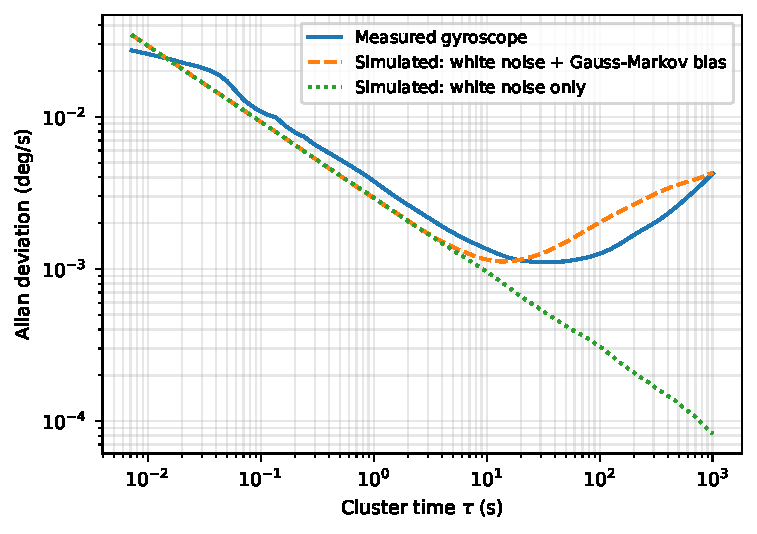
\includegraphics[width=0.75\textwidth]{allan_variance}
\caption{Gyroscope Allan deviation: measured (1.95 million samples at
\SI{140}{Hz}, stationary) against data simulated from
\eqref{eq:sensormodel}--\eqref{eq:walkingbias} with the parameters of
Table~\ref{tab:noise}, and against white noise alone.}
\label{fig:allan}
\end{figure}

\rev{\begin{remark}[The sample rate trade]\label{rem:dttrade}
The encoder velocity quantization interacts with the sample rate in the opposite
direction from everything else. Halving $\Delta t$ improves the fidelity of
\eqref{eq:zoh} but doubles the velocity quantization noise. There is therefore
an interior optimum in $\Delta t$ for a fixed encoder resolution, and raising the
loop rate without raising the encoder resolution eventually degrades the
velocity estimate. A procedure for locating this optimum from logged data is
given in Appendix~\ref{app:validation}.
\end{remark}}

\section{NONLINEARITIES}

The Pololu DC motors exhibit several obvious nonlinearities that can be
accounted for in simulation. Friction is an important nonlinearity to consider,
but owing to the difficulty of evaluating the forces and obtaining an accurate
model it was left out of the simulation; its effect is absorbed into $d_1$ and
$d_2$ and forms part of what the networks estimate.

\subsection{Saturation}

The commanded voltage is limited by the supply rail,
\begin{equation}\label{eq:sat}
\mathrm{sat}(u)=
\begin{cases}
u_{\max}, & u>u_{\max},\\
u, & \abs{u}\le u_{\max},\\
-u_{\max}, & u<-u_{\max}.
\end{cases}
\end{equation}
Saturation is applied to the control signal output in all simulation cases.

\subsection{Deadzone}

Below a threshold voltage the motor does not turn. The standard deadzone model
is continuous at the breakaway points, but the physical motors exhibit a jump
discontinuity: the output steps to a finite value at breakaway rather than
rising continuously from zero. The model used is
\begin{equation}\label{eq:deadzone}
\mathcal{D}(u)=
\begin{cases}
m_d\bigl(u-\delta_+\bigr)+j_+, & u>\delta_+,\\
0, & -\delta_-\le u\le\delta_+,\\
m_d\bigl(u+\delta_-\bigr)-j_-, & u<-\delta_- ,
\end{cases}
\end{equation}
with $\delta_\pm$ the breakaway voltages, $m_d$ the slope outside the deadband,
and $j_\pm$ the jump magnitudes.

\begin{figure}[htbp]
\centering
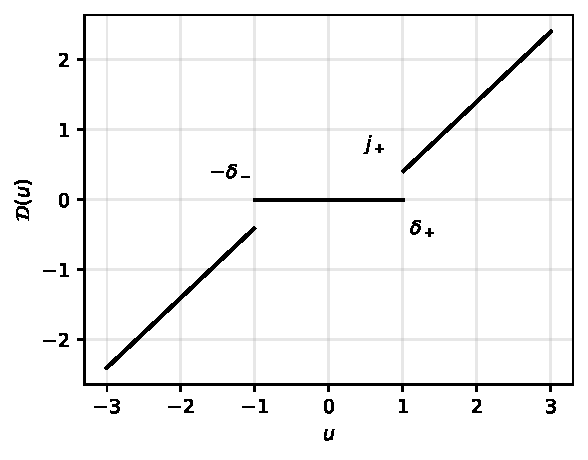
\includegraphics[width=0.55\textwidth]{deadzone}
\caption{Deadzone nonlinearity with jump discontinuities.}
\label{fig:deadzone}
\end{figure}

\subsection{Backlash}

Gear backlash is modeled as hysteresis \cite{tao1993backlash,durdevic2013hybrid} in which the output holds while the input
reverses through a deadband of half-width $\Delta_b$,
\begin{equation}\label{eq:backlash}
\dot y=
\begin{cases}
m_b\dot u, & \dot u>0 \text{ and } y=m_b\bigl(u-\Delta_b\bigr),\\
m_b\dot u, & \dot u<0 \text{ and } y=m_b\bigl(u+\Delta_b\bigr),\\
0, & \text{otherwise.}
\end{cases}
\end{equation}

\begin{figure}[htbp]
\centering
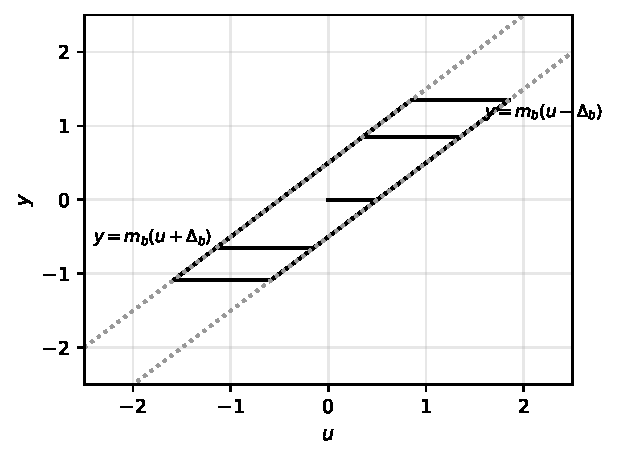
\includegraphics[width=0.55\textwidth]{backlash}
\caption{Backlash nonlinearity: response to a decaying sinusoidal input with
$m_b=1$, $\Delta_b=0.5$.}
\label{fig:backlash}
\end{figure}

\rev{\begin{remark}[Backlash is outside the approximation hypothesis]
\label{rem:backlash}
On the physical robot the backlash was measured at less than one degree of
output-shaft rotation, although the recorded runs show a stick-slip limit cycle
near upright (Section~\ref{sec:momtest}). Two observations follow. First, because the encoders are
mounted on the motor shaft, this deadband is invisible to the measurement, so it
appears to the estimator as an unmodeled input nonlinearity rather than as a
measurable state discrepancy. Second, \eqref{eq:backlash} is not smooth and
therefore violates the smoothness assumption underlying
Assumption~\ref{as:nn}. The networks can approximate it only in an averaged
sense, and the residual appears in $\epsilon_N$ and in $w_{i0}$. This is the
correct explanation for the persistent oscillation in the uncertainty estimates
reported in Chapter~\ref{ch:results}: the limit cycle is the signature of a
nonsmooth input nonlinearity that no smooth approximator can cancel, not a
tuning failure.
\end{remark}}

\section{DISCRETE KALMAN FILTER}
\label{sec:dkf}

The discrete Kalman filter is used for comparison against the DMSO. The Kalman
filter, developed by Kalman in 1960, provides the statistically optimal state
estimate for a linear system with measurements corrupted by Gaussian,
zero-mean, uncorrelated, white noise \cite{kalman1960}. The filter processes
measurements together with knowledge of the system dynamics to produce a more
accurate state estimate. The version used here is the discrete-time filter and
follows Simon \cite{simon2006optimal}.

Assume the dynamic system is given by
\begin{equation}\label{eq:kfplant}
x_{k+1}=Fx_k+Gu_k+w_k ,
\end{equation}
with measurements
\begin{equation}\label{eq:kfmeas}
y_k=Hx_k+v_k ,
\end{equation}
where $w_k$ and $v_k$ are zero-mean, uncorrelated, white Gaussian sequences with
\begin{equation}\label{eq:kfstats}
w_k\sim\mathcal{N}\bigl(0,Q_{\mathrm{K}}\bigr),
\qquad
v_k\sim\mathcal{N}\bigl(0,R_{\mathrm{K}}\bigr).
\end{equation}
$Q_{\mathrm{K}}$ is the process noise covariance and $R_{\mathrm{K}}$ the
measurement noise covariance; both may be adjusted for performance. States with
greater uncertainty in the dynamics can be assigned larger values in
$Q_{\mathrm{K}}$, which causes the filter to weight the measurements more
heavily. $R_{\mathrm{K}}$ can be obtained accurately by statistical analysis of
the available measurements.

The filter is given by the update equations
\begin{align}
P_{k+1}^-&=FP_k^+F^T+Q_{\mathrm{K}},\label{eq:kf1}\\[2pt]
L_{k+1}&=P_{k+1}^-H^T\bigl(HP_{k+1}^-H^T+R_{\mathrm{K}}\bigr)^{-1},\label{eq:kf2}\\[2pt]
\xhat_{k+1}^-&=F\xhat_k^++Gu_k ,\label{eq:kf3}\\[2pt]
\xhat_{k+1}^+&=\xhat_{k+1}^-+L_{k+1}\bigl(y_{k+1}-H\xhat_{k+1}^-\bigr),\label{eq:kf4}\\[2pt]
P_{k+1}^+&=\bigl(I-L_{k+1}H\bigr)P_{k+1}^-\bigl(I-L_{k+1}H\bigr)^T
+L_{k+1}R_{\mathrm{K}}L_{k+1}^T ,\label{eq:kf5}
\end{align}
where the superscripts $-$ and $+$ denote a priori and a posteriori quantities,
$P$ is the estimation error covariance, $L$ is the Kalman gain, and $\xhat$ the
state estimate. The equations are processed sequentially from \eqref{eq:kf1} to
\eqref{eq:kf5}. Equation \eqref{eq:kf5} is the Joseph form, which preserves
symmetry and positive definiteness of the covariance under finite-precision
arithmetic. Measurements need not arrive at the same rate as the dynamics are
propagated; \eqref{eq:kf4} may be processed only at intervals where measurements
are available. In the simulations here the measurements are assumed available at
the dynamics rate.

\rev{\subsection{Three Baselines}

A comparison between the DMSO and a Kalman filter must be constructed carefully
to be meaningful. The Kalman filter is optimal for a linear system driven by
zero-mean white process noise of known covariance. It is not designed to reject
a deterministic modeling error, and demonstrating that it fails to do so
establishes little about the DMSO. Three baselines are therefore used in
Chapter~\ref{ch:results}:
\begin{enumerate}[label=(\alph*),leftmargin=*]
\item a Kalman filter with $Q_{\mathrm{K}}$ tuned to the sensor noise alone,
which is the naive baseline and the one used in revision~7;
\item a Kalman filter with $Q_{\mathrm{K}}$ inflated to account for the
parameter error, which is what a competent practitioner would actually do;
\item an augmented-state Kalman filter in which the uncertainty is modeled as a
random-walk state and estimated alongside the dynamic states, which is the
closest linear analogue of the DMSO and the fairest comparison.
\end{enumerate}
For baseline (c) the state is augmented as
$x^{\mathrm{aug}}=\begin{bmatrix}x^T&f^T\end{bmatrix}^T$ with
\begin{equation}\label{eq:augkf}
F^{\mathrm{aug}}=\begin{bmatrix}F&\Bm\\0&I_p\end{bmatrix},
\qquad
G^{\mathrm{aug}}=\begin{bmatrix}G\\0\end{bmatrix},
\qquad
H^{\mathrm{aug}}=\begin{bmatrix}H&0\end{bmatrix},
\end{equation}
and the process noise covariance on the appended block set to the assumed
random-walk intensity of the uncertainty. Claims of improvement are stated
against (c).}

\chapter{RESULTS}
\label{ch:results}

\rev{The corrections in Chapters~\ref{ch:dmso} and~\ref{ch:control} change the
admissible gain ranges and, in the control case, the structure of the law
itself, so the results are regenerated here rather than carried over from
revision~7. All simulations and hardware replays in this chapter are produced by
the open-source Python implementation accompanying this thesis
(\texttt{twip-dmso}; script \texttt{scripts/thesis\_rev8.py}), which also records
every number quoted below.}

\section{TEST MATRIX AND METRICS}
\label{sec:testmatrix}

\subsection{Cases}

Each case is run for both the observer study and the control study.

\begin{table}[htbp]
\centering
\caption{Simulation test matrix}
\label{tab:testmatrix}
\begin{tabular}{clccc}
\toprule
Case & Description & Noise & Param.\ error & Nonlinearity \\
\midrule
O1 & Nominal & --- & --- & --- \\
O2 & Parameter uncertainty & --- & \checkmark & --- \\
O3 & Noise and uncertainty & \checkmark & \checkmark & --- \\
O4 & Unmodeled dynamics & \checkmark & \checkmark & --- \\
C1 & Control, nominal & \checkmark & --- & --- \\
C2 & Control, uncertainty & \checkmark & \checkmark & --- \\
C3 & Control, deadzone & \checkmark & \checkmark & deadzone \\
C4 & Control, deadzone + backlash & \checkmark & \checkmark & both \\
\bottomrule
\end{tabular}
\end{table}

\subsection{Simulation setup}
\label{sec:setup}

\rev{The truth model is the nonlinear model of Section~\ref{sec:simmodel},
integrated with fourth-order Runge--Kutta at one tenth of the
$\Delta t=\SI{10}{ms}$ loop period of the hardware. The estimators and
controllers use the nominal linearization discretized by \eqref{eq:zoh}.

\emph{Parameter error.} Cases O2--O4 and C2--C4 propagate the truth with
$M_p\times1.1$, $M_w\times1.5$, $k_m\times1.25$, $k_e\times0.95$, and $R\times1.2$;
the observer and controller retain the nominal values. This is the
perturbation of the revision~7 extra-control study with the torque-constant
error reduced from $\times2.5$ to $\times1.25$. With the corrected model of
Section~\ref{sec:simmodel}, the nominal LQR cannot stabilize the revision~7
perturbation even with perfect state knowledge, and a comparison of estimators
on a plant that no controller holds upright is not informative.

\emph{Unmodeled dynamics.} Case O4 adds the revision~7 unmodeled terms
$0.5\sin(x_1)x_2$ to $\dot x_2$ and $0.25x_2^2$ to $\dot x_4$.

\emph{Observer study.} For each case a single truth trajectory is generated by
the LQR of Section~\ref{sec:lqr} acting on the \emph{true} state, tracking a
position sinusoid of amplitude \SI{0.3}{m} and period \SI{8}{s} from an initial
tilt of \SI{5}{\degree}, for \SI{30}{s}. Every estimator then processes the same
measurement and input sequences, so all are compared on identical information.
The measurement $y_k$ is the full state as the robot constructs it: the encoder
position and velocity corrected for body tilt, the complementary-filtered tilt
of \eqref{eq:compfilter}, and the gyroscope rate. Without noise, $y_k=x_k$.
Each estimator is scored by its one-step prediction of $x_{k+1}$ after
processing $y_k$ and $u_k$, which is the native output of the DMSO and is
formed for the Kalman filters as $F\xhat_{k|k}+Gu_k$. The uncertainty truth is
$f_k=\Bm^T\bigl(x_{k+1}-Fx_k-Gu_k\bigr)$ computed from the true state.

\emph{Control study.} Each controller closes the loop itself for \SI{20}{s},
from \SI{5}{\degree} of tilt at rest, tracking a constant velocity of
\SI{0.1}{m/s}. The state is supplied to every controller by the same
Kalman filter, which models the accelerometer kinematics as described in
Section~\ref{sec:simmodel}. The LQR includes the nominal steady-state
feedforward voltage for the commanded velocity. Case C3 uses a
\SI{0.5}{V} deadzone and C4 adds an input backlash of half-width
$\Delta_b=\SI{0.25}{V}$.}

\subsection{Metrics}

\rev{Scalar summaries are reported per case rather than averaged across cases.
An average of percentage improvements taken over heterogeneous scenarios is not
a meaningful statistic, since the scenarios have different error scales and the
mean is dominated by whichever case happens to have the smallest baseline.}
The reported metrics are, for each state and each case:
\begin{enumerate}[label=(\roman*),leftmargin=*]
\item RMS estimation error over the run, after excluding the first
\SI{5}{s} as initial transient;
\item time to first entry into the ultimate bound predicted by
\eqref{eq:bounds}, together with that predicted bound;
\item RMS regulation or tracking error for the control cases;
\item RMS and peak control effort, to confirm that improvements are not bought
with unreported actuator authority.
\end{enumerate}

\subsection{Verification of the theoretical conditions}

\rev{Each run records $\sigmax(A)$, $\phi_{\max}$ as realized along the
trajectory, and the product $\Gamma\phi_{\max}^2$, so that satisfaction of
\eqref{eq:simple} can be confirmed rather than assumed.}

\rev{The DMSO is configured by the constructive procedure of
Appendix~\ref{app:validation}. The error-injection gain is $\Km=F-\bar\sigma I$,
so that $A=\bar\sigma I$ is normal and $\sigmax(A)=\bar\sigma=0.5$ exactly. The
basis is $\phi(y)=\bigl[1,\ \tanh(y_1/1),\ \tanh(y_2/1),\ \tanh(y_3/0.2),\
\tanh(y_4/1)\bigr]^T$, which is bounded by construction with
$\phi_{\max}^2=5$. The adaptation gain is one tenth of the bound
\eqref{eq:simple}, $\Gamma=0.01$. Table~\ref{tab:obscond} confirms that the
conditions hold along every trajectory; the realized $\phi_{\max}^2$ never
exceeds $2.2$, well below its design value.}

\begin{table}[htbp]
\centering
\caption{DMSO stability conditions as realized in each observer case}
\label{tab:obscond}
\small
\begin{tabular}{lccccccc}
\toprule
Case & $\sigmax(A)$ & $\phi_{\max}^2$ (design) & $\phi_{\max}^2$ (realized) & $\Gamma$
     & $\Gamma\phi_{\max}^2$ & bound on $\Gamma$ & \eqref{eq:simple} holds \\
\midrule
O1 & 0.50 & 5 & 1.86 & 0.0100 & 0.0186 & 0.100 & yes \\
O2 & 0.50 & 5 & 2.01 & 0.0100 & 0.0201 & 0.100 & yes \\
O3 & 0.50 & 5 & 2.19 & 0.0100 & 0.0219 & 0.100 & yes \\
O4 & 0.50 & 5 & 2.20 & 0.0100 & 0.0220 & 0.100 & yes \\
\bottomrule

\end{tabular}
\end{table}

\section{OBSERVER RESULTS}

\rev{Six estimators are compared: the three Kalman baselines of
Section~\ref{sec:dkf}; the revision~7 DMSO (basis on $\xhat_k$, $\Km=I$,
$\Gamma=0.1$) for reference; and the revision~8 DMSO, with and without
$\sigma$-modification ($\kappa=0.1$). A seventh row, marked $\dagger$, uses the
same adaptation law with the steady-state Kalman gain as error injection,
$\Km=FL$, so that $A=F(I-L)$. That $A$ is Schur but strongly non-normal
($\sigmax(A)=1.04$ without noise and $6.3$ with it), so Theorem~\ref{thm:main}
does not apply in the Euclidean norm and the row is an empirical extension;
see Remark~\ref{rem:nonnormal} and Section~\ref{sec:obsdiscussion}.}

\subsection{Nominal and parameter-uncertainty cases}

\rev{In case O1 there is no model error and every estimator predicts the state
to within numerical precision (Figure~\ref{fig:O1}); the DMSO weights remain
near zero because there is nothing to learn.

Case O2 is the setting the DMSO is designed for: a deterministic model error and
a noise-free measurement. Figure~\ref{fig:O2} shows the norm of the estimation
error against the ultimate bound of Theorem~\ref{thm:main}. The bound requires
$\epsilon_N$; a valid value on the realized trajectory is the largest residual
of a least-squares fit of the true uncertainty onto the basis,
$\epsilon_N=0.0113$, which gives $b_e=0.0235$. The error enters the bound after
0.12~s and remains inside it from 0.86~s onward. The excursions before that are
the initial transient, which Theorem~\ref{thm:main} does not constrain.

The DMSO identifies the uncertainty itself, not only the state
(Figure~\ref{fig:O2unc}). Against the augmented-state Kalman filter, the
baseline against which improvement is claimed, the RMS error of $\fhat$ is
lower by a factor of 11 in both the velocity and the tilt-rate channel
(Table~\ref{tab:obsunc}). The one-step prediction error of the uncertain states
is lower by a factor of 5 in both channels (Table~\ref{tab:obsrms}). Relative to
the revision~7 observer, the corrected basis and adaptation law reduce the
uncertainty estimation error by a factor of about 3. $\sigma$-modification
costs accuracy here, as the analysis predicts, because the leakage biases
the weights toward zero while the uncertainty is persistently nonzero.}

\begin{figure}[htbp]
\centering
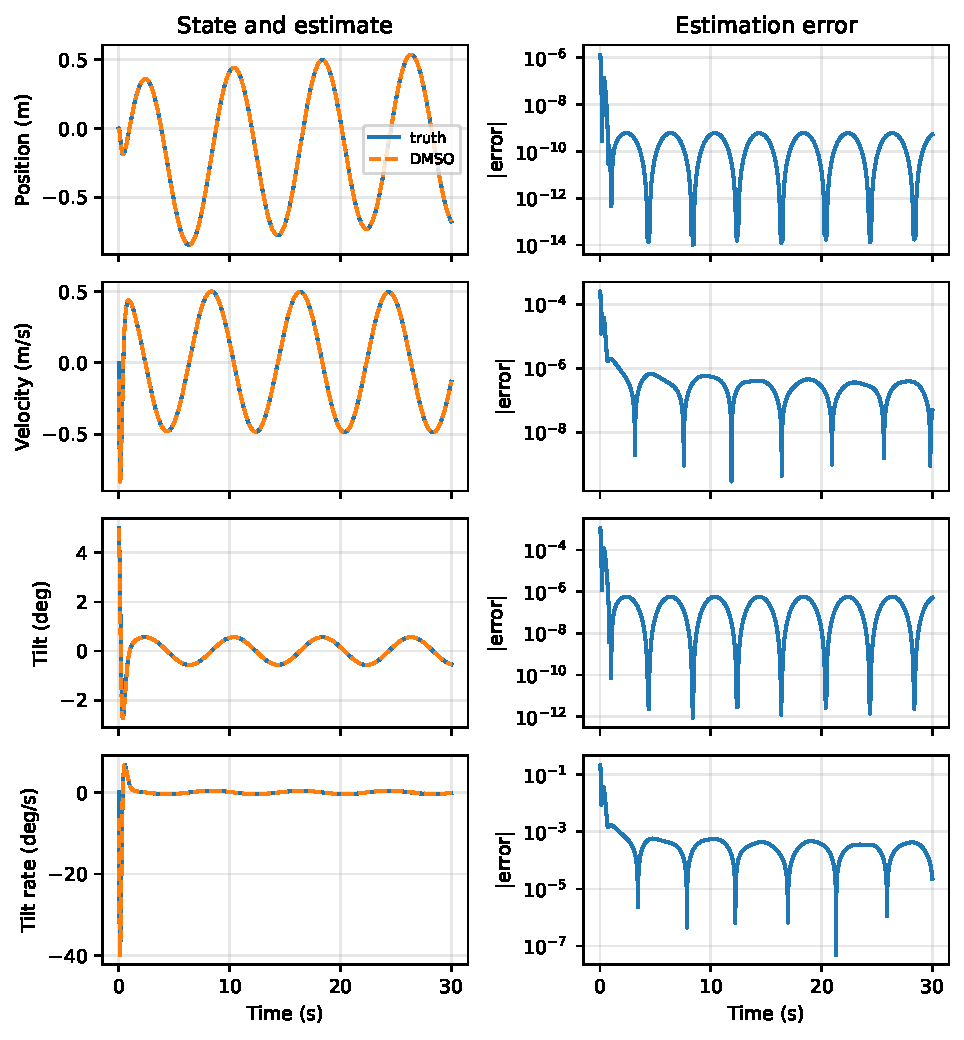
\includegraphics[width=0.85\textwidth]{O1}
\caption{Case O1: states, DMSO one-step predictions, and prediction error.}
\label{fig:O1}
\end{figure}

\begin{figure}[htbp]
\centering
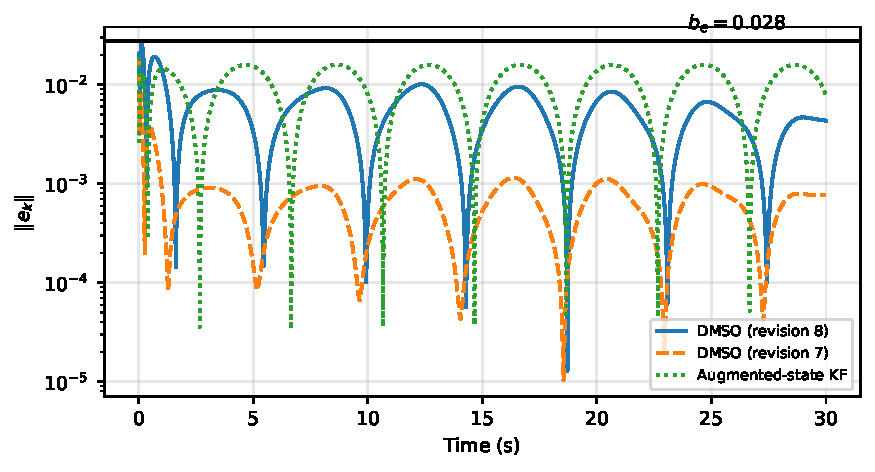
\includegraphics[width=0.85\textwidth]{O2_bound}
\caption{Case O2: norm of the estimation error with parameter uncertainty,
against the predicted ultimate bound $b_e$ of \eqref{eq:bounds}.}
\label{fig:O2}
\end{figure}

\begin{figure}[htbp]
\centering
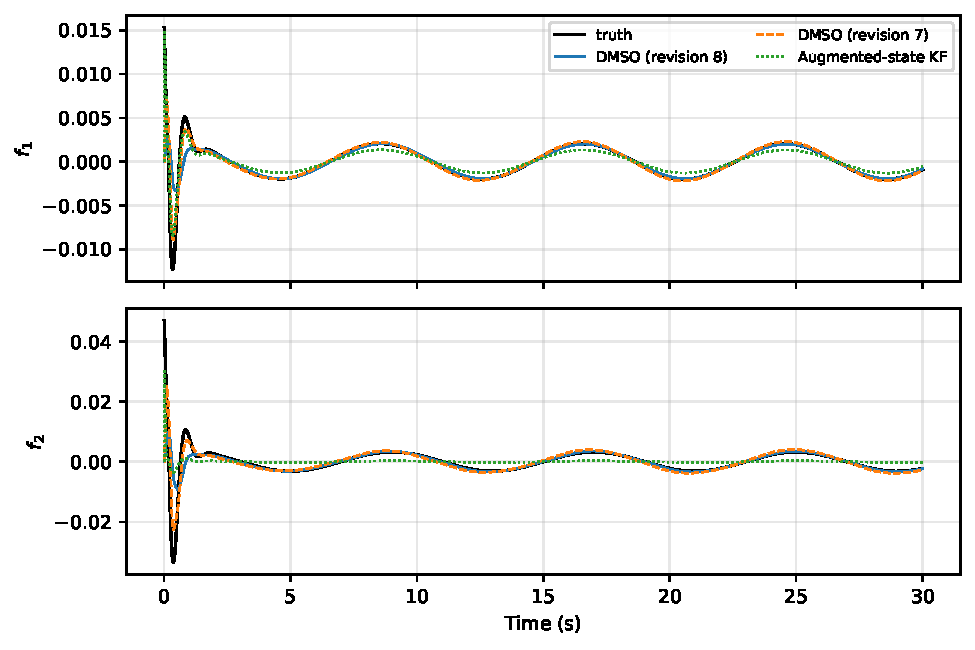
\includegraphics[width=0.85\textwidth]{O2_uncertainty}
\caption{Case O2: DMSO uncertainty estimates against truth, with the revision~7
DMSO and the augmented-state Kalman filter for comparison.}
\label{fig:O2unc}
\end{figure}

\subsection{Cases with sensor noise}

\rev{With sensor noise the picture is mixed, and it is reported as such
(Figure~\ref{fig:O3} and Table~\ref{tab:obsrms}).

In the velocity channel the DMSO remains better than both unaugmented Kalman
filters, by a factor of 2.5 in case O3, and is within 40\% of the
augmented-state filter. In the tilt channel it is an order of magnitude worse
than the two unaugmented filters and comparable to the augmented one. The cause is the measurement rather than the adaptation.
The complementary-filtered tilt carries a slowly varying error of about
\SI{1.1}{\degree} RMS, because the accelerometer measures tilt relative to the
apparent vertical, which is displaced by the robot's own acceleration. With
$A=\bar\sigma I$ the DMSO corrects each channel only from its own measurement,
and so it follows that error. The Kalman filters instead infer tilt through
the model from the measured wheel acceleration, which the $A_2x_3$ coupling
makes available.

The Kalman-gain variant ($\dagger$) combines the two mechanisms. Its velocity
and tilt errors lie between those of the unaugmented and augmented filters, and
its tilt-rate error is 30\% above the nominal filter's in O3 and equal to it in
O4. It gives the best
uncertainty estimate in the noisy cases: 1.4 times lower
than the augmented filter in the velocity channel of O3, and 3 to 4 times lower
in the tilt-rate channel. Its gain lies outside the conditions of
Theorem~\ref{thm:main}, so these numbers are empirical.

In the tilt-rate channel of the noisy cases, every estimator's uncertainty error
is comparable to or larger than the RMS of the true uncertainty itself
(Table~\ref{tab:obsunc}). At this
noise level, $f_2$ is not identifiable from the available measurements by any
of the six estimators; only $f_1$ is.}

\begin{figure}[htbp]
\centering
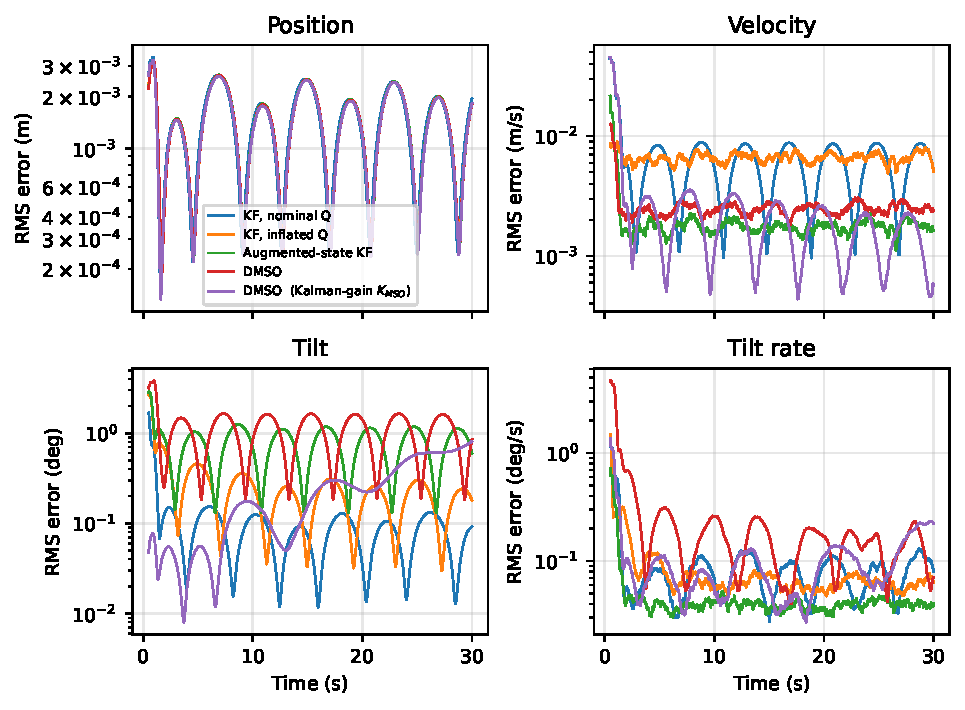
\includegraphics[width=0.9\textwidth]{O3}
\caption{Case O3: estimation error (\SI{0.5}{s} moving RMS), DMSO against the
three Kalman baselines of Section~\ref{sec:dkf}.}
\label{fig:O3}
\end{figure}

\begin{table}[htbp]
\centering
\caption{Observer RMS one-step prediction error by case and estimator:
velocity (\si{mm/s}) / tilt (\si{mrad}) / tilt rate (\si{mrad/s}). Position
errors are set by the encoder quantization and are identical across
estimators (\SI{1.6}{mm} in O3 and O4).}
\label{tab:obsrms}
\scriptsize
\setlength{\tabcolsep}{3pt}
\begin{tabular}{lcccc}
\toprule
Estimator & O1 & O2 & O3 & O4 \\
\midrule
KF, nominal $Q_{\mathrm{K}}$ & $<$0.01 / $<$0.01 / $<$0.01 & 1.43 / 0.01 / 2.29 & 6.22 / 1.55 / 1.41 & 4.74 / 1.34 / 1.42 \\
KF, inflated $Q_{\mathrm{K}}$ & $<$0.01 / $<$0.01 / $<$0.01 & 1.43 / 0.01 / 2.29 & 6.63 / 3.81 / 1.10 & 6.42 / 3.68 / 1.12 \\
Augmented-state KF & $<$0.01 / $<$0.01 / $<$0.01 & 0.49 / 0.02 / 2.06 & 1.77 / 14.49 / 0.69 & 1.84 / 14.09 / 0.69 \\
DMSO, revision 7 & $<$0.01 / $<$0.01 / 0.01 & 0.14 / 0.01 / 0.54 & 6.17 / 20.09 / 1.25 & 6.08 / 19.48 / 1.21 \\
DMSO & $<$0.01 / $<$0.01 / 0.01 & 0.09 / 0.02 / 0.38 & 2.48 / 20.13 / 2.85 & 2.44 / 19.52 / 3.03 \\
DMSO with $\sigma$-mod & $<$0.01 / $<$0.01 / $<$0.01 & 0.61 / 0.02 / 0.88 & 2.71 / 20.13 / 4.91 & 2.60 / 19.52 / 5.10 \\
DMSO, Kalman-gain $\Km$\,$^\dagger$ & $<$0.01 / $<$0.01 / $<$0.01 & 0.96 / 0.06 / 1.47 & 1.97 / 6.51 / 1.86 & 2.05 / 3.95 / 1.39 \\
\bottomrule

\end{tabular}\\[2pt]
{\footnotesize $^\dagger$ outside the conditions of Theorem~\ref{thm:main}; empirical.}
\end{table}

\begin{table}[htbp]
\centering
\caption{RMS uncertainty estimation error $\fhat-f$ ($\times10^{-3}$),
velocity channel / tilt-rate channel. Only estimators that produce an
uncertainty estimate are listed; O1 has no uncertainty.}
\label{tab:obsunc}
\small
\begin{tabular}{lccc}
\toprule
Estimator & O2 & O3 & O4 \\
\midrule
Augmented-state KF & 0.69 / 11.27 & 0.59 / 7.28 & 0.59 / 7.25 \\
DMSO, revision 7 & 0.11 / 0.75 & 1.22 / 11.65 & 1.22 / 11.61 \\
DMSO & 0.44 / 2.81 & 0.94 / 11.44 & 0.94 / 11.36 \\
DMSO with $\sigma$-mod & 0.52 / 3.25 & 1.12 / 12.57 & 1.14 / 12.51 \\
DMSO, Kalman-gain $\Km$\,$^\dagger$ & 1.41 / 8.84 & 0.84 / 9.47 & 0.88 / 9.38 \\
\midrule
RMS of true $f$ & 1.99 / 12.38 & 1.99 / 12.38 & 1.98 / 12.24 \\
\bottomrule

\end{tabular}
\end{table}

\subsection{Discussion}
\label{sec:obsdiscussion}

\rev{Three conclusions follow. First, the corrected DMSO does what the analysis
claims. Its conditions are satisfied with margin, its error settles inside the
predicted bound, and under deterministic model error it identifies the
uncertainty an order of magnitude more accurately than the fairest Kalman
baseline. Second, the choice $A=\bar\sigma I$, which makes the proof simplest,
discards the cross-channel information that a model-based filter exploits. When
one measurement carries a structured error, that choice costs more than the
adaptation gains. Third, Theorem~\ref{thm:main} admits any $\Km$ with
$\sigmax(F-\Km)<1$, and the empirical success of the Kalman-gain injection
suggests extending the proof through the weighted norm of
Remark~\ref{rem:nonnormal}. That extension is not immediate. With
$V_k=e_k^TT^TTe_k+\Gamma^{-1}\norm{\Wt_k}_F^2$, the cancellations of
Proposition~\ref{prop:exact} survive only if the adaptation law is weighted
correspondingly, $\What_{k+1}=\What_k+\Gamma\phi_ke_{k+1}^TT^TT\Bm$, and if
$\Bm^TT^TT\Bm=I$. Those conditions should be imposed explicitly.}

\section{CONTROL RESULTS}

\subsection{Realizability of the command-filtered design}
\label{sec:cfinstab}

\rev{The command-filtered design of Section~\ref{sec:cffb} could not be
stabilized, and the reason is structural. Stage~3 of
Appendix~\ref{app:validation} was followed: the backstepping structure was run
first with both networks disabled, on the nominal linear model, with perfect
state knowledge and no saturation. The closed loop diverged within seven samples.

Linearizing the continuous-time closed loop (plant and three command filters,
networks disabled) gives a real eigenvalue near $+7$~rad/s for every gain set
tried: 720 combinations of $c_1,\dots,c_4$ and $\varpi_1,\varpi_2,\varpi_3$, including
all combinations satisfying \eqref{eq:gaincond}. The smallest value found for
the largest real part was $+6.35$~rad/s. As the filter bandwidths are raised,
that eigenvalue converges to $+7.23$~rad/s (Figure~\ref{fig:chi}), which is the
right-half-plane transmission zero of the position-to-voltage transfer function
$x_1(s)/u(s)$. On the revision~7 parameters the zero is at $+6.11$~rad/s, so the
difficulty does not come from the model corrections.

The mechanism is the following. With $x_1$ as the tracked output, the recursion
drives all four error coordinates to zero, which requires the closed loop to
invert the plant from $u$ to $x_1$. For a non-minimum-phase output, that
inversion places a closed-loop pole at the zero. In the analysis the
instability is hidden in Assumption~\ref{as:filt}. The virtual control
$\alpha_2$ contains $B_1u$, the control depends on the filter state
$\dot x_4^c$, and $\alpha_3$ contains $\dot x_3^c$. So $\alpha_2$ and its
derivatives depend on the filter errors themselves, and the premise that
$\alpha_i$ and $\dot\alpha_i$ are bounded, which yields
$\chi_i=O(1/\varpi_i)$, does not follow from the construction. Raising the
bandwidth moves the unstable eigenvalue toward the zero rather than into the
left half-plane.

Two remedies preserve the intent of Section~\ref{sec:cffb}. The first is to
track a minimum-phase output. For a controllable single-input linearization, the
flat output $y=Cx$ with $CB=CAB=CA^2B=0$ has relative degree four and no zero
dynamics, and a four-step recursion on it is well posed. The second is a
cascade: a position loop slower than the zero that commands tilt, and a
backstepping tilt loop with the network compensation. The control table below
therefore reports the command-filtered design as unrealizable in its present
form.}

\begin{figure}[htbp]
\centering
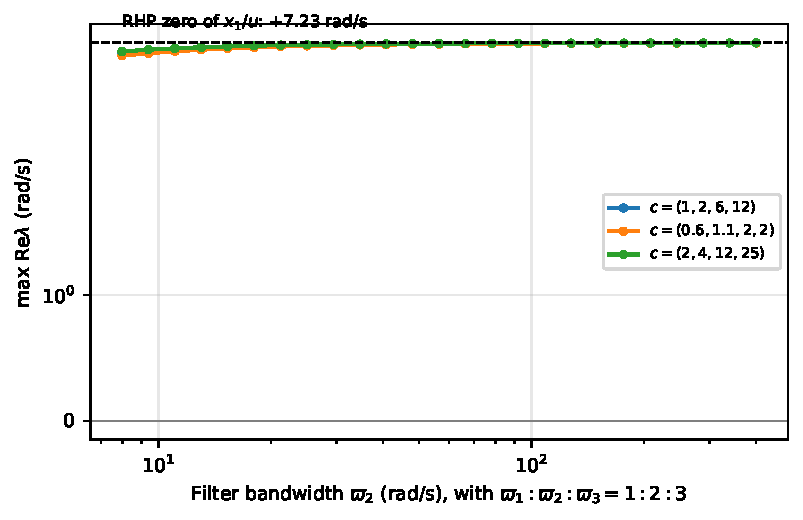
\includegraphics[width=0.8\textwidth]{cfb_eigenvalues}
\caption{Largest real part of the closed-loop eigenvalues of the command-filtered
design (networks disabled, nominal linear model) against the command-filter
bandwidth, for three sets of damping gains. The dashed line is the
right-half-plane zero of $x_1(s)/u(s)$. Assumption~\ref{as:filt} requires the
filter errors $\chi_i$ to shrink as $\varpi_i$ grows; instead the unstable
eigenvalue converges to the zero.}
\label{fig:chi}
\end{figure}

\subsection{LQR and the two-step extra control}

\rev{Table~\ref{tab:ctrleff} and Figures~\ref{fig:C2}--\ref{fig:C4} compare
the LQR alone with the revision~7 two-step extra control. The two-step design
is the \texttt{ExtraControl\_v5.m} law with $k_{e0}=0$, the setting that
reproduces the revision~7 figures.

The two-step extra control reduces the RMS position tracking error by 17\% in
the nominal case C1 and by 30\% under deadzone and backlash (C4). It increases
it by 4\% with parameter uncertainty alone (C2) and by 22\% with the deadzone
(C3). It uses between 1\% and 29\% more RMS control. Both controllers balance in
every case. In both, the position error is dominated by the slow position
mode of the LQR (the thesis weights place a closed-loop pole at
$|\lambda|=0.9995$ at \SI{10}{ms}). Under the deadzone it is also dominated by a
steady velocity deficit that neither design removes, visible as the ramp in
Figure~\ref{fig:C4}.

A slow position ramp, the behavior Remark~\ref{rem:twostep} predicts for the
two-step design, appears in cases C2--C4. It appears equally for the LQR alone,
with slopes of 0.02 to \SI{0.06}{m/s} for both controllers over the last
\SI{10}{s}. So it is not a property of the two-step design. It is the
velocity error left by an incorrect steady-state feedforward under parameter
error, integrated by a position loop too weak to remove it. Test T3 of
Appendix~\ref{app:validation} therefore neither confirms nor refutes
Remark~\ref{rem:twostep}. The LQR term supplies whatever position damping
there is in both designs.}

\begin{figure}[htbp]
\centering
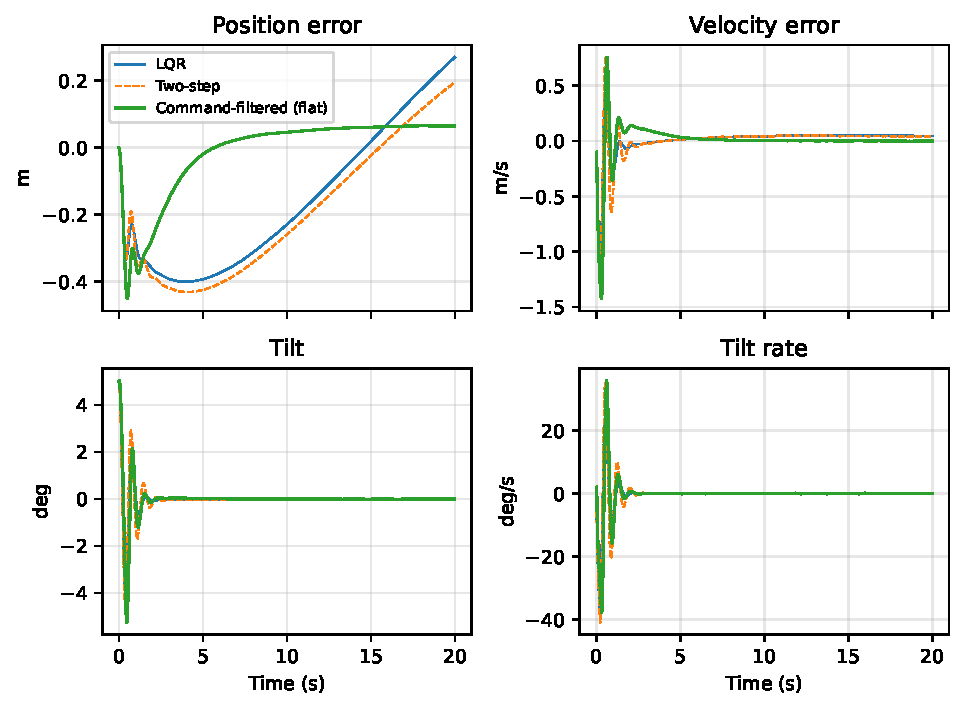
\includegraphics[width=0.85\textwidth]{C2}
\caption{Case C2: position and velocity tracking errors, tilt, and tilt rate
with and without the two-step extra control.}
\label{fig:C2}
\end{figure}

\begin{figure}[htbp]
\centering
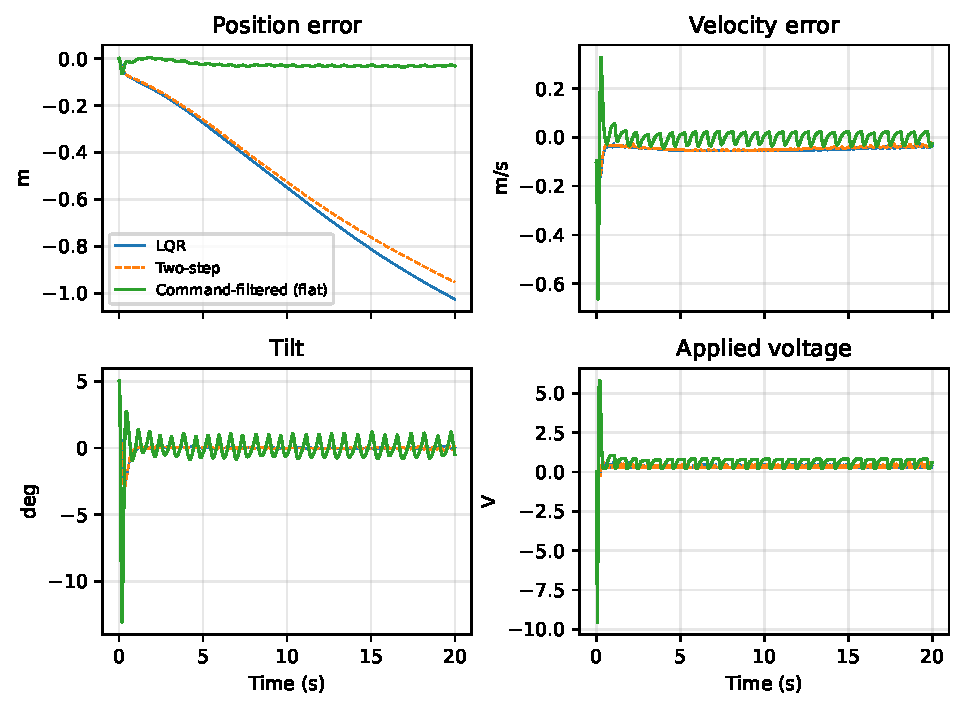
\includegraphics[width=0.85\textwidth]{C4}
\caption{Case C4: response under deadzone and backlash.}
\label{fig:C4}
\end{figure}

\begin{table}[htbp]
\centering
\caption{Control effectiveness by case: RMS position tracking error (\si{m})
after \SI{5}{s} / RMS voltage (\si{V}) / peak voltage (\si{V}).}
\label{tab:ctrleff}
\footnotesize
\setlength{\tabcolsep}{4pt}
\begin{tabular}{lcccc}
\toprule
Controller & C1 & C2 & C3 & C4 \\
\midrule
LQR alone & 0.055 / 0.72 / 2.6 & 0.068 / 0.73 / 2.6 & 0.091 / 0.74 / 2.6 & 0.680 / 0.39 / 2.3 \\
LQR + two-step (rev.~7) & 0.051 / 0.72 / 2.6 & 0.068 / 0.73 / 2.6 & 0.100 / 0.75 / 2.6 & 0.647 / 0.41 / 2.3 \\
Command-filtered, flat output, networks off & 0.004 / 0.93 / 9.7 & 0.016 / 0.90 / 9.6 & 0.016 / 0.91 / 9.7 & 0.033 / 0.93 / 9.6 \\
Command-filtered, flat output, networks on & 0.004 / 0.93 / 9.7 & 0.016 / 0.90 / 9.6 & 0.016 / 0.91 / 9.7 & 0.031 / 0.93 / 9.6 \\
Command-filtered, as in Section~\ref{sec:cffb} & \multicolumn{4}{c}{unstable for all gains tested (Section~\ref{sec:cfinstab})} \\
\bottomrule

\end{tabular}
\end{table}

\section{IMPLEMENTATION RESULTS}
\label{sec:implresults}

\rev{The hardware results are replays of the logged LQR run
\texttt{implementationtest5.txt}, recorded with firmware v9 at a
\SI{10}{ms} loop. Figure~\ref{fig:hw} compares the measured states, the
estimates computed on board by the v9 DMSO (which the replay reproduces to
print precision), and the revision~8 DMSO run offline on the same data. After
the first second the three agree to within the measurement quantization. There
is no truth on hardware, so the replays establish consistency, not accuracy.}

\begin{figure}[htbp]
\centering
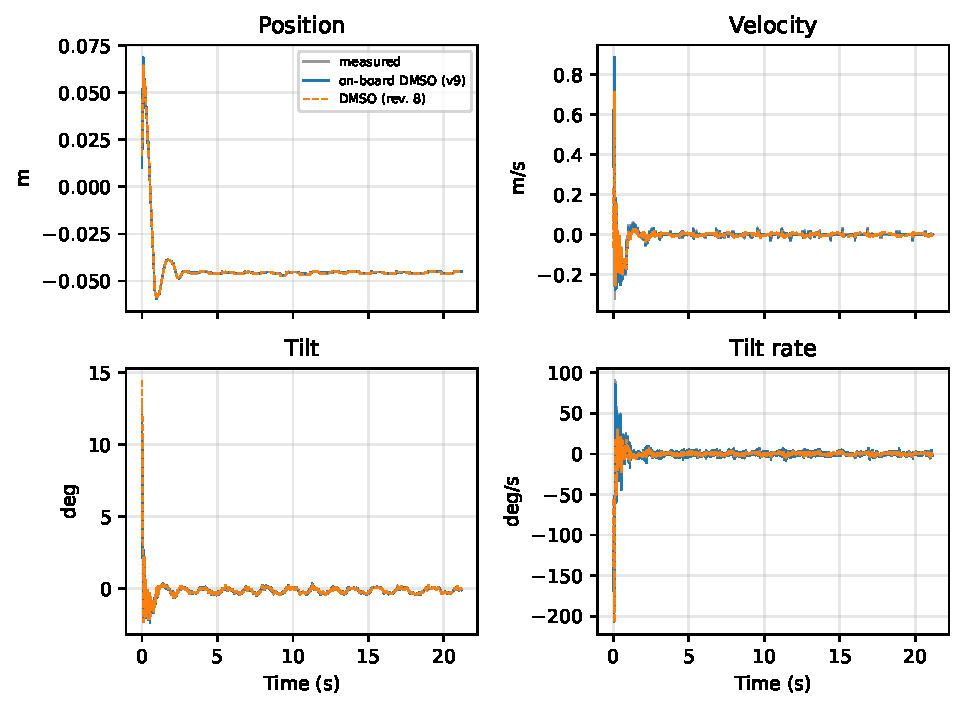
\includegraphics[width=0.85\textwidth]{hw_states}
\caption{Hardware test: measured states, on-board (v9) DMSO estimates, and the
revision~8 DMSO replayed offline.}
\label{fig:hw}
\end{figure}

\begin{figure}[htbp]
\centering
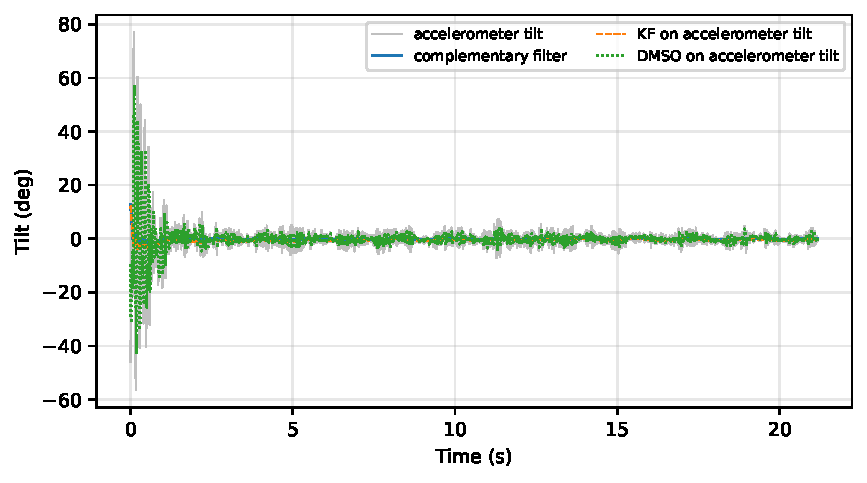
\includegraphics[width=0.85\textwidth]{hw_complementary}
\caption{Hardware test: complementary filter against the model-based estimators
using raw accelerometer tilt.}
\label{fig:complementary}
\end{figure}

\begin{figure}[htbp]
\centering
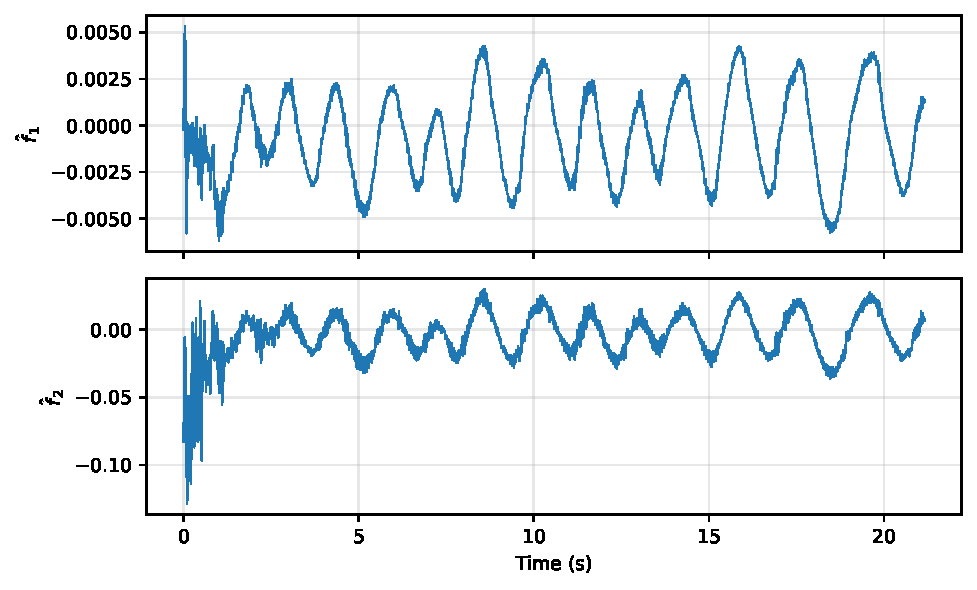
\includegraphics[width=0.85\textwidth]{hw_uncertainty}
\caption{Hardware test: DMSO uncertainty estimates.}
\label{fig:hwunc}
\end{figure}

\rev{The revision~7 result that the complementary filter outperforms the
model-based estimators fed raw accelerometer tilt is re-examined in
Figure~\ref{fig:complementary}. Without truth, each tilt estimate is scored
by its consistency with the gyroscope, the RMS of
$\dd\hat\theta/\dd t-g_y$. This measures high-frequency error and is blind to
slow bias. On that score the raw accelerometer tilt is at
\SI{476}{\degree/s}, the complementary filter at \SI{9.9}{\degree/s}, and the
DMSO fed raw accelerometer tilt at \SI{295}{\degree/s}. The Kalman filter fed
the same raw tilt, with a measurement variance that reflects its actual error,
reaches \SI{4.2}{\degree/s}.

The finding therefore holds for the DMSO but not for a correctly weighted
Kalman filter. The explanation needs no gearbox transients: an accelerometer
measures tilt relative to the apparent vertical, which is displaced by
$\ddot x/g$ whenever the robot accelerates. An estimator that corrects each
channel from its own measurement follows that displacement, and one that
weights the measurement by its true error does not. The conclusion of
revision~7 stands in modified form: it is a statement about measurement
construction and error-injection design, not about the adaptation.

Figure~\ref{fig:hwunc} shows the uncertainty estimated on hardware. The
tilt-rate channel is several times larger than in simulation (RMS
$1.4\times10^{-2}$ against $2.3\times10^{-3}$), consistent with the model
error on the physical robot being larger than the simulated perturbation.
Appendix~\ref{app:validation} describes how to settle this by measurement.}

\chapter{CONCLUSIONS}
\label{ch:conclusions}

The Modified State Observer has been extended to discrete time and its stability
established by Lyapunov analysis. \rev{The proof evaluates the first difference
of the Lyapunov function exactly, which exposes the cancellations that the
adaptation law was constructed to produce. The resulting conditions are
$\sigmax(F-\Km)<1$ together with an upper bound on the adaptation gain, both
satisfiable over an open set of designs, and both reducing to the expected
limiting behavior as the adaptation gain tends to zero. The analysis bounds the
state estimation error and the functional approximation error
$\Wt_k^T\phi_k$; boundedness of the weight estimate itself follows either from
persistency of excitation or, without that requirement, from
$\sigma$-modification of the update law.}

\rev{In simulation on the corrected robot model, the observer satisfies its
conditions with margin, settles inside the predicted ultimate bound, and under
deterministic parameter error identifies the uncertainty an order of magnitude
more accurately than an augmented-state Kalman filter. With realistic sensor
noise the advantage is confined to the velocity channel. The diagonal error
injection that makes the proof simplest cannot use the model to reject the
structured error of the accelerometer-derived tilt, which a Kalman-gain
injection recovers empirically.}

\rev{A command-filtered neural backstepping controller has been developed for
the two-wheeled inverted pendulum, an underactuated system with unmatched
uncertainty. The design assigns damping to every error coordinate, retains and
explicitly cancels the coupling between the position and attitude error
subsystems, and uses command filtering so that each network approximates a
function of measured state and reference alone. Its boundedness result is
conditional on the command-filter error assumption. For the TWIP that
assumption does not hold: tracking the non-minimum-phase position output
places a closed-loop pole at the right-half-plane zero of $x_1(s)/u(s)$, and the
design could not be stabilized. The revision~7 two-step extra control does
balance the robot in every case, with mixed effect on tracking accuracy.}

Four directions follow naturally from this work.

\paragraph{A realizable backstepping output.} \rev{Repeating the four-step
construction on the flat output $y=Cx$, $CB=CAB=CA^2B=0$, which has no zero
dynamics, or restructuring it as a cascade with a position loop slower than the
zero, would retain the damping and command-filtering ideas of
Chapter~\ref{ch:control} while removing the obstruction identified in
Section~\ref{sec:cfinstab}.}

\paragraph{Output feedback.} The present development assumes full state
measurement, so the DMSO is properly a filter and uncertainty identifier. The
structure of Proposition~\ref{prop:exact} carries over to $y_k=Cx_k$ with
$A=F-\Km C$, and the extension requires only a detectability assumption. This
is the most direct route to a result that applies to systems where the tilt rate
or the wheel velocity is not directly measured.

\paragraph{Nonsmooth input nonlinearities.} Backlash violates the smoothness
assumption underlying the universal approximation property, and the residual
limit cycles observed both in simulation and on hardware are its signature. A
network cannot cancel what it cannot approximate. Two remedies are worth
pursuing: an explicit deadzone- and backlash-inverse placed ahead of the plant,
or a discontinuous term in the control law that is robust to the deadband rather
than attempting to estimate it.

\paragraph{Deterministic timing.} \rev{The achievable sample rate on the
platform was set by telemetry rather than by the control computation, and the
encoder velocity quantization scales inversely with the sample period. Both are
implementation choices rather than properties of the algorithm, and both bound
what any estimator can deliver. Appendix~\ref{app:validation} treats the loop
rate as a design variable and gives the trade.}


\appendix
\chapter{IMPLEMENTATION AND VALIDATION GUIDANCE}
\label{app:validation}

This appendix gives a staged procedure for implementing and testing the observer
of Chapter~\ref{ch:dmso} and the controller of Chapter~\ref{ch:control}. The
organizing principle is that each stage must have a falsifiable pass criterion
that is checkable without the next stage being correct. A design that is
assembled all at once and then tuned until it balances provides no evidence
about which component is working.

\section{STAGE 0: PARAMETER IDENTIFICATION}

The detuning of the LQR gains reported in Section~\ref{sec:difficulties} is
evidence of parameter error, and the two parameters most likely responsible are
the pendulum inertia $I_p$ and the CG offset $l$. Both can be measured directly
and should be, before any estimator is judged.

\paragraph{Procedure.} Remove the wheels and suspend the chassis from a knife
edge at the wheel axis so that it swings as a physical pendulum. Record the
small-amplitude period $T$ with the onboard gyroscope. Then
\begin{equation}\label{eq:pendid}
T=2\pi\sqrt{\frac{I_{\mathrm{pivot}}}{M_pgl}},
\qquad
I_{\mathrm{pivot}}=I_p+M_pl^2 .
\end{equation}
Measure $l$ independently by balancing the chassis on a knife edge to locate the
CG, then solve \eqref{eq:pendid} for $I_p$. Repeat at several amplitudes to
confirm the small-angle regime.

\paragraph{Motor constants.} Measure $R$ by four-wire resistance at a dozen
shaft positions and average, since commutator position changes the reading.
Obtain $k_e$ by back-driving the motor at a measured rate and reading the
open-circuit terminal voltage; $k_e$ from the slope of $V$ against
$\dot\vartheta$ is far more reliable than $k_e$ inferred from catalog free-run
and stall figures. For a brushed DC motor in SI units $k_m=k_e$, and any
substantial discrepancy between a measured $k_e$ and a catalog-derived $k_m$
indicates that one of the two is wrong.

\paragraph{Deadzone and backlash.} Ramp the commanded voltage slowly in both
directions with the wheels off the ground and record the breakaway voltages
$\delta_+$ and $\delta_-$ of \eqref{eq:deadzone}. Measure backlash by holding
the motor shaft and rotating the wheel through the deadband, reading the
free rotation directly; this gives $\Delta_b$ in \eqref{eq:backlash}.

\rev{\paragraph{Sign conventions.} Hold the wheels on the ground and rotate the
body by hand in the positive sense of $\phi$ (counterclockwise in
Figure~\ref{fig:fbdpend}, center of gravity moving toward $-x$). The logged tilt
should increase, and the encoder count should change in the same sense as when
the robot rolls forward, since the encoders read $x/r+\phi$
(Section~\ref{sec:simmodel}). These two signs fix the tilt compensation of the
encoder position, $x=\mathrm{pos}-r\phi$, used in the estimators and in the
replays of Section~\ref{sec:implresults}; with either reversed, the compensation
doubles the tilt term instead of removing it.}

\paragraph{Pass criterion.} The LQR gains computed from the measured parameters
stabilize the hardware without manual detuning. If they do not, the model is
still wrong and no amount of online estimation will make the comparison in
Chapter~\ref{ch:results} interpretable.

\section{STAGE 1: OFFLINE ESTIMATOR REPLAY}

Before the observer is allowed to influence any control signal, run it open
loop on recorded data.

\begin{enumerate}[label=\arabic*.,leftmargin=*]

\item Drive the robot with the LQR controller alone and log, at the full loop
rate, the raw gyroscope and accelerometer samples, the raw encoder counts, the
commanded voltage, and a timestamp taken from a hardware timer rather than from
a software counter.

\item Replay the log offline through the DMSO. Because $y_k=x_k$ here, the
observer can be evaluated without closing any loop.

\item Verify the theoretical conditions numerically on the replayed data:
compute $\sigmax(F-\Km)$ for the $\Delta t$ actually achieved, compute
$\phi_{\max}=\max_k\norm{\phi(x_k)}$ realized along the recorded trajectory, and
confirm \eqref{eq:simple}. \rev{This is the step most often skipped. The
$\phi_{\max}$ used to select $\Gamma$ is a design assumption, and the trajectory
is free to violate it.}

\end{enumerate}

\paragraph{Pass criterion.} The estimation error settles inside the predicted
ultimate bound $b_e$ of \eqref{eq:bounds}, and $\Gamma\phi_{\max}^2$ computed
from realized data satisfies \eqref{eq:simple}. If the error settles but the
bound is violated, the gains are outside the proven region and the result is
empirical only.

\section{STAGE 2: OBSERVER GAIN SELECTION}

The conditions of Corollary~\ref{cor:theta1} give a constructive selection
order.

\begin{enumerate}[label=\arabic*.,leftmargin=*]

\item \textbf{Place $A$ first.} Choose $\Km$ so that $\sigmax(F-\Km)$ takes a
target value $\bar\sigma$. Note that $\sigmax$, not the eigenvalues, is what
matters; a gain that places the eigenvalues of $A$ well inside the unit circle
can still have $\sigmax(A)>1$ if $A$ is strongly non-normal. Compute the
singular values explicitly. A practical starting point is
$\bar\sigma\in[0.5,0.8]$. \rev{Smaller values reject model error faster, with a
response time that scales as $1/\log(1/\bar\sigma)$, and lower the model-error
floor $\epsilon_N/(1-\bar\sigma)$ of \eqref{eq:limbounds}. Their cost is
measurement noise, which Theorem~\ref{thm:main} does not model: as $\bar\sigma$
falls, $\Km=F-\bar\sigma I$ approaches $F$ and the prediction follows each noisy
measurement more closely. That side of the trade has to be judged from data.}

\item \textbf{Bound $\phi_{\max}$ by construction.} Rather than estimating
$\phi_{\max}$ from a nominal trajectory, choose activation functions that are
bounded by construction, for example a Gaussian radial basis or a
$\tanh$ polynomial basis, so that $\phi_{\max}$ is known a priori and
independent of how far the trajectory wanders.

\item \textbf{Select $\Gamma$ from \eqref{eq:simple}.} With $\bar\sigma$ and
$\phi_{\max}$ fixed,
\[
\Gamma<\frac{1}{\phi_{\max}^2}\min\left\{\frac{1}{2},\,
\frac{1-\bar\sigma^2}{2\bar\sigma^2}\right\}.
\]
Begin at one tenth of this bound and increase. \rev{The speed of uncertainty
identification is set by $\Gamma$, and the conditions permit any sufficiently
small value, so there is no reason to operate near the boundary.}

\item \textbf{Add $\sigma$-modification.} Use \eqref{eq:sigmod} with
$\kappa$ chosen so that $\Gamma\kappa\ll1$; a decade below $\Gamma$ is a
reasonable start. \rev{This is strongly recommended over relying on persistency
of excitation. During regulation about the upright equilibrium the regressor is
nearly constant and \eqref{eq:pe} will not hold, which is exactly the condition
under which weight drift occurs. Drift is insidious: the state estimate remains
good while the weights wander, and the failure appears only when the trajectory
eventually excites a direction the drifted weights misrepresent.}

\end{enumerate}

\paragraph{Diagnostic.} Log $\norm{\What_k}_F$ throughout every run. A weight
norm that grows slowly and monotonically while the estimation error stays small
is the signature of drift, and it is the reason to add leakage rather than to
increase $\Gamma$.

\section{STAGE 3: CONTROLLER BRING-UP}

The controller of Section~\ref{sec:flatcf} \rev{(the structure of
Section~\ref{sec:cffb} in flat-output coordinates)} has four damping gains,
three filter bandwidths, four learning rates, and four leakage gains. Bring them up in this
order, and only in this order.

\begin{enumerate}[label=\arabic*.,leftmargin=*]

\item \textbf{LQR alone.} Confirm stable regulation with the measured
parameters from Stage~0. Record the baseline metrics of
Section~\ref{sec:testmatrix}.

\item \textbf{Backstepping with networks disabled.} Set $\hat F_1=\hat F_2=0$
and run the structure of Section~\ref{sec:flatcf} with $u_e$ active. This tests
the command filters, the error coordinate bookkeeping, and the sign conventions
without any adaptation. \rev{Most implementation errors in a backstepping design
are sign errors in the cross-term cancellations, and they are far easier to find
with the adaptation off.} \rev{Verify numerically that the implemented error
dynamics are the derived ones: difference the logged $z_i$ to estimate
$\dot z_i$, evaluate the right-hand sides of the error equations of
Section~\ref{sec:flatcf} from the logged signals, and confirm that the two agree
to within the discretization error. A sign error in a cancelling pair, such as
$a_2z_3$ in $\dot z_2$ against $-(a_2/w)z_2$ in $\dot z_3$, appears as a residual
proportional to one of the coordinates. (Logging expressions such as
$z_1z_2-z_2z_1$ is not a test: they are zero for any numbers.)} If the two do not
agree, the implementation does not match the derivation.

\item \textbf{Filter bandwidths.} Raise $\varpi_i$ until $\chi_i$ is small
relative to the corresponding $z_i$, then stop. \rev{With noisy measurements
$\chi_i$ stops shrinking, and can grow, as the bandwidth rises
(Figure~\ref{fig:chi}b), so raise $\varpi_i$ only while $\chi_i$ falls.} The upper limit is the lesser of
one fifth of the sample rate and the lowest unmodeled structural mode of the
chassis. \rev{The stiffening rods described in
Section~\ref{sec:difficulties} exist because that mode was originally low enough
to contaminate the inertial measurements; it should be measured, not assumed,
by striking the chassis and recording the gyroscope response.}

\item \textbf{One network at a time.} Enable network one with network two
disabled, then the reverse, then both. Each network has its own error
coordinate driving it, $z_2$ and $z_4$ respectively, so a network that is not
helping shows up as a failure to reduce its own coordinate.

\item \textbf{Leakage last.} Raise $\kappa_{ij}$ only as far as needed to hold
the weight norms flat over a long run. Every increase adds
$\kappa_{ij}W_{ijm}^2/2$ to the residual $\mathcal{C}$ in
\eqref{eq:Vdotfinal} and therefore to the steady-state error.

\end{enumerate}

\section{STAGE 4: HARDWARE ARCHITECTURE}

Two limitations identified in Section~\ref{sec:difficulties} are architectural
rather than algorithmic, and both bound what any estimator can achieve.

\subsection{Separate the control path from the telemetry path}

Serial transmission dominated the loop budget. The remedy is to make the control
path deterministic and the telemetry path best-effort:

\begin{itemize}[leftmargin=*]
\item Run the control law from a hardware timer interrupt at fixed period, and
do no I/O inside it beyond sensor reads and the actuator write.
\item Write telemetry into a ring buffer from the interrupt and drain the buffer
from the main loop, so that a slow or blocked link cannot extend the control
period.
\item Log to onboard storage at full rate and stream a decimated subset, rather
than streaming everything.
\item Timestamp from a free-running hardware counter, not from a software
accumulator, so that jitter is measurable after the fact. \rev{Report the
achieved loop period distribution, not its nominal value. The discretization
\eqref{eq:zoh} assumes a fixed $\Delta t$, and jitter enters as an unmodeled
disturbance that the networks will attempt, and fail, to explain.}
\end{itemize}

\subsection{The encoder placement limits the achievable result}

The encoders are on the motor shaft, ahead of the gearbox, so backlash is
structurally unobservable. \rev{Increasing the loop rate does not help: the
measurement is not noisy, it is measuring the wrong thing.} Two remedies are
available, in increasing order of effort:

\begin{enumerate}[label=(\alph*),leftmargin=*]
\item \textbf{Load-side encoding.} Add a second encoder on the output shaft or
the wheel. The difference between motor-side and load-side angle is then a
direct measurement of the backlash state, which converts an unmodeled
nonlinearity into an observable quantity and permits an explicit backlash
inverse. This is the single highest-value hardware change available.
\item \textbf{Deterministic timing in hardware.} Implementing the fixed-point
control law in programmable logic removes scheduler jitter entirely and permits
loop rates well beyond what the microcontroller supports. This is worth doing
only after (a); a faster loop around a blind measurement does not improve the
estimate.
\end{enumerate}

\subsection{The sample rate trade}

\rev{There is an interior optimum in $\Delta t$ and it should be found rather
than assumed. Shortening $\Delta t$ improves the fidelity of \eqref{eq:zoh} and
reduces the interval over which the zero-order hold is in error, but the encoder
velocity quantization in Table~\ref{tab:noise} scales as
$1.47\times10^{-4}/\Delta t$, so the velocity measurement degrades linearly as
the loop speeds up. Sweep $\Delta t$ in replay over the logged data from
Stage~1, plot the RMS velocity estimation error against $\Delta t$, and operate
at the minimum. If the minimum lies at the shortest $\Delta t$ tested, the
encoder resolution is not the binding constraint and the loop rate may be raised
further; if it lies in the interior, raising the loop rate requires raising the
encoder resolution first.}

\section{STAGE 5: FALSIFICATION TESTS}

Each of the following is designed to fail if a specific claim is untrue.

\begin{enumerate}[label=T\arabic*.,leftmargin=*]

\item \textbf{Bound verification.} Run case O2 with a deliberately inflated
parameter error and confirm that the estimation error settles inside $b_e$ from
\eqref{eq:bounds} computed with the realized $\phi_{\max}$. A violation means
either the conditions are not met or the implementation does not match the
derivation.

\item \textbf{Small-gain admissibility.} Run the observer at
$\Gamma$ one and two decades below the bound in \eqref{eq:simple}. \rev{Stability
must be retained, with slower identification. This test directly falsifies the
revision~7 condition, which excluded small gains, and confirms the corrected
one.}

\item \textbf{Position drift.} Run cases C2 and C4 for at least ten times the
dominant closed-loop time constant with the two-step and command-filtered
designs side by side, and plot $z_1$ over the full run. \rev{Remark~\ref{rem:twostep} predicts
that the two-step design permits a slow position ramp. Either it appears, which
confirms the analysis, or it does not, which means the LQR term is supplying the
missing damping and should be credited explicitly in the design rather than
absorbed into the approximation targets.}

\item \textbf{Algebraic loop.} Disable the command filters, replacing $x_3^c$
with $\alpha_2$ directly, and attempt to execute the ordering of
Remark~\ref{rem:order}. \rev{The computation should fail to be well posed. This
confirms that the filters are structural rather than cosmetic.}

\item \textbf{Weight drift.} Run a long regulation case with leakage disabled
and log $\norm{\What_k}_F$. Growth in the weight norm with a flat estimation
error confirms that persistency of excitation does not hold in regulation and
justifies $\sigma$-modification.

\item \textbf{Nonsmoothness floor.} Run case C4 with the backlash amplitude
$\Delta_b$ swept over a range including zero. \rev{The residual limit cycle
amplitude should scale with $\Delta_b$ and vanish as $\Delta_b\to0$. If it does
not, the limit cycle has another cause and the explanation in Remark~\ref{rem:backlash} is wrong.}

\end{enumerate}

\section{SOFTWARE ORGANIZATION}

A structure that supports the above is worth stating explicitly.

\begin{itemize}[leftmargin=*]
\item \textbf{One model, three consumers.} The continuous model
\eqref{eq:nl1}--\eqref{eq:nl2}, the discretization \eqref{eq:zoh}, and the
parameter set should exist in exactly one place and be consumed by the truth
propagator, the estimator, and the controller. Divergence between a simulation
model and a flight model is a classic and silent source of error.
\item \textbf{Same source, both targets.} The estimator and controller should
compile for both the desktop simulation and the embedded target from the same
source, with the platform differences confined to sensor and actuator
interfaces. This makes replay meaningful: the code that is tested is the code
that runs.
\item \textbf{Fixed-point discipline early.} If the eventual target is
fixed-point, introduce the scaling in simulation and compare against the
floating-point result, rather than discovering the scaling problems on
hardware.
\item \textbf{Record the conditions, not just the results.} Every run should
emit $\sigmax(A)$, realized $\phi_{\max}$, $\Gamma\phi_{\max}^2$, the achieved
loop period distribution, and the weight norms, alongside the state histories.
These are what make a result checkable a year later.
\end{itemize}

\chapter{TECHNICAL CHANGES FROM REVISION 7}
\label{app:errata}

This appendix records the specific technical differences between this revision
and revision~7, with the equation numbers of the earlier document given for
reference.

\section{CHAPTER 3: THE DMSO STABILITY PROOF}

\paragraph{B.1.1 Bound on $\norm{I-\Gamma\phi\phi^T}$ (was Eq.~22).}
Revision~7 used
$\norm{(I-\Gamma\phi\phi^T)\Wt}^2\le(1-\Gamma\norm{\phi}^2)^2\norm{\Wt}^2$. The
matrix $I-\Gamma\phi\phi^T$ is symmetric with eigenvalue $1$ of multiplicity
$l-1$ and eigenvalue $1-\Gamma\norm{\phi}^2$ of multiplicity one, so its induced
$2$-norm is $\max\{1,\abs{1-\Gamma\norm{\phi}^2}\}$, which equals $1$ whenever
$\Gamma\norm{\phi}^2\le2$. The factor used was strictly smaller than the true
norm, so the step was not conservative but invalid. Substituting the correct
value makes the coefficient of $\norm{\Wt_k}^2$ in the former Eq.~(23) equal to
$2/\alpha+3\phi_{\max}^2>0$, and the argument cannot close in that form.

\paragraph{B.1.2 Gain conditions (was Eqs.~26--27).}
Substituting the choice $\alpha=1/(3\phi_{\max}^2)$ into the former Eq.~(26)
gives
\begin{equation}\label{eq:persq}
\frac{2}{\alpha}-6\frac{\Gamma}{\alpha}\phi_{\max}^2
+3\frac{\Gamma^2}{\alpha}\phi_{\max}^4+3\phi_{\max}^2
=9\phi_{\max}^2\bigl(1-\Gamma\phi_{\max}^2\bigr)^2\ \ge\ 0 ,
\end{equation}
a perfect square, whereas the condition required the expression to be
nonpositive. The only admissible point is the boundary
$\Gamma=1/\phi_{\max}^2$, at which the coefficient is zero rather than negative.
The reported condition $\Gamma\le1/\phi_{\max}^2$ was therefore satisfied by no
interior point and excluded small gains, which is the opposite of the correct
behavior established in Theorem~\ref{thm:main} and Corollary~\ref{cor:theta1}.

\paragraph{B.1.3 Weight bound (was Eq.~33).}
The bound inherited the denominator
$-9\phi_{\max}^2(1-\Gamma\phi_{\max}^2)^2\le0$ from \eqref{eq:persq} and was
therefore either undefined or infinite. It is replaced by the honest statement
of Theorem~\ref{thm:main}, which bounds $\Wt_k^T\phi_k$, together with
Section~\ref{sec:weightbound}, which obtains boundedness of $\Wt_k$ from
persistency of excitation or $\sigma$-modification.

\paragraph{B.1.4 Matrix norm (was above Eq.~23).}
Revision~7 used $\norm{A}\le\lmax(A)$. The induced $2$-norm is the largest
singular value, and $\sigmax(A)\ge\rho(A)$, with equality for normal $A$ (and
for some non-normal $A$).
For $A=F-\Km$ the inequality is generally strict and $\lmax(A)$ may be complex.
See Remark~\ref{rem:nonnormal}.

\paragraph{B.1.5 The matrix $Q$ (was after Eq.~28).}
With $P=I$ in the discrete Lyapunov equation $A^TPA-P=-Q$, one has
$Q=I-A^TA$ and $\lmin(Q)=1-\sigmax(A)^2$, so $Q$ is determined by $A$ and is not
independently selectable. The former condition then reduces to
$\sigmax(A)^2\le1/(3+9\Gamma^2\phi_{\max}^4)$, requiring
$\sigmax(A)\lesssim0.29$ at $\Gamma\phi_{\max}^2=1$. The corrected condition is
$\sigmax(A)<1$.

\paragraph{B.1.6 Structural cause.}
Applying Young's inequality to the first difference before evaluating the trace
difference discards the cancellations established in
Proposition~\ref{prop:exact}, which are precisely what the adaptation law was
constructed to produce.

\paragraph{B.1.7 What the Lyapunov argument concludes.} \rev{The first
difference is negative outside a set that bounds $e_k$ and $\psi_k$ but not the
components of $\Wt_k$ orthogonal to $\phi_k$, so that set is not compact in the
observer state $(e_k,\Wt_k)$ and the Lyapunov extension theorem does not apply to
it directly. Theorem~\ref{thm:main} now states a mean-square bound
\eqref{eq:msbound} that needs no bound on the weights, and uniform ultimate
boundedness under a bound on $\Wt_k$ from Section~\ref{sec:weightbound}. The
same applies to Corollary~\ref{cor:deadbeat}. Assumption~\ref{as:nn} now states
that the plant trajectory remains in the compact set on which the approximation
holds, and Remark~\ref{rem:nonnormal} states that a weighted Lyapunov function
requires a correspondingly weighted adaptation law.}

\section{CHAPTER 6: THE EXTRA CONTROL DESIGN}

\paragraph{B.2.1 Missing coupling term (was Eqs.~97 and 100).}
The former Eq.~(97) was obtained by substituting $x_3=\bar x_3$ from the former
Eq.~(93), and was then reused in Eq.~(100) in a setting where $x_3\ne\bar x_3$
by construction. Carrying $x_3=\bar x_3+\bar e_3$ through leaves a term
$+A_2\bar e_3$ in $\dot{\bar e}_2$ that did not appear in the error dynamics or
in the Lyapunov derivative. In the present design this term is retained as
$A_2z_3$ in \eqref{eq:z2dot} and cancelled by the $-A_2z_2$ term in
\eqref{eq:alpha3}.

\paragraph{B.2.2 Undamped error coordinates (was Eqs.~122 and 138--140).}
In revision~7 the cross terms $\bar e_1^T\bar e_2$ and $\bar e_3^T\bar e_4$
cancelled, removing $\bar e_1$ and $\bar e_3$ from the Lyapunov derivative
entirely, and the stated conditions involved only $\norm{\bar e_2}$ and
$\norm{\bar e_4}$. Uniform ultimate boundedness requires the derivative to be
negative outside a compact set in the full error space, which cannot hold in a
direction absent from the derivative. Since $\dot{\bar e}_1=\bar e_2$ is a pure
integrator, a bounded but nonvanishing $\bar e_2$ permits $\bar e_1$ to ramp.
The four-step design of Section~\ref{sec:cffb} assigns damping to all four
coordinates.

\paragraph{B.2.3 Circular approximation targets (was Eqs.~96 and 104).}
The former $F_1$ contained $B_1u_e$, with $u_e$ a function of $\hat F_2$, while
the former $F_2$ contained $-\dot{\bar x}_4$, which contains derivatives of
$\hat F_1$ and hence of the weight estimates. Neither target was a fixed
continuous function of its network input, so the universal approximation
hypothesis did not apply. The targets \eqref{eq:F1} and \eqref{eq:F2} contain no
control signal and no adaptive parameter; the command filters of
Section~\ref{sec:cmdfilter} supply the required derivative signals as filter
states and break the algebraic loop, as detailed in Remark~\ref{rem:order}.

\paragraph{B.2.4 Unmatched first-layer weights (was Eqs.~122 and 134).}
The hidden-layer activation error $\tilde\sigma_{i2}$ was bounded by a constant
$W_{i2m}\sigma_{i2m}$, so the first-layer weight error never appeared in the
Lyapunov derivative and the first-layer update law was unjustified by the
analysis. Equation \eqref{eq:nnerr} uses the standard two-layer Taylor form in
which both layers' weight errors appear linearly and are matched term by term by
the update laws \eqref{eq:upd2}--\eqref{eq:upd1}.

\paragraph{B.2.5 Sign convention (was Eqs.~111--114).}
The two layers carried opposite overall signs in the update laws. Both laws in
\eqref{eq:upd2}--\eqref{eq:upd1} now use the same convention.

\paragraph{B.2.6 Riccati equation (was Eq.~83).}
The trailing factor was written as $A$, a carryover from continuous-time
notation. It is $F$, the discretized system matrix; see \eqref{eq:dare}.

\paragraph{B.2.7 Gain conditions and network residual.} \rev{The state $z_2$
carries two cross terms in the Lyapunov derivative, the filter error and the
residual of network one, so Theorem~\ref{thm:control} requires $c_2>1$, as its
proof always concluded. The Taylor residual $w_i$ of \eqref{eq:nnerr} contains
the weight errors and is bounded by $w_{i0}+w_{i1}\norm{\Wt_i}_F$, not by a
constant; the $\sigma$-modification leakage absorbs the weight-dependent part
when $\kappa_{ij}>2w_{i1}^2$, which is now part of \eqref{eq:gaincond}.}

\section{FRAMING AND REPORTING}

\paragraph{B.3.1 Observer or filter.}
With $y_k=x_k$ the full state is measured. The method is a filter and
uncertainty identifier rather than an observer in the unmeasured-state sense,
and this is now stated explicitly.

\paragraph{B.3.2 Kalman filter comparison.}
Comparing against a Kalman filter that is given no mechanism to accommodate a
deterministic modeling error establishes little. Three baselines are now used,
including an augmented-state filter that estimates the uncertainty as a random
walk, and improvement claims are stated against that one.

\paragraph{B.3.3 Aggregated percentages.}
An average percentage improvement taken over heterogeneous cases is not a
meaningful statistic. Metrics are now reported per case.

\paragraph{B.3.4 Complementary filter result.}
The finding that the complementary filter outperforms both model-based
estimators when those are fed raw accelerometer tilt is retained and explained:
it is a statement about measurement construction, not about estimator quality.
\rev{Re-examined on the hardware data in Section~\ref{sec:implresults}, it holds
for the DMSO but not for a Kalman filter whose measurement variance reflects
the actual accelerometer tilt error.}

\section{MODEL AND RESULTS}

\paragraph{B.4.1 Plant model.} \rev{Four corrections enter the simulations of
Chapter~\ref{ch:results}. The motor torque reacts on the pendulum with positive
sign in the counterclockwise moment balance \eqref{eq:pendm}; revision~7 had the
opposite sign, which changes the back-EMF and input terms of \eqref{eq:nl1},
\eqref{eq:lin1}, and \eqref{eq:linss}. The corrected input vector satisfies the
angular-momentum check of Remark~\ref{rem:momentum}, and the free swing of
Section~\ref{sec:modelsim} is lightly rather than strongly damped. The remaining
three are in Section~\ref{sec:simmodel}: the back-EMF acts on the wheel rate
relative to the body, $\dot x/r+\dot\phi$; $k_e=\SI{0.307}{V.s/rad}$ from the
free-run data in place of \SI{0.00361}{V.s/rad}; and $I_p$ is taken about the
center of gravity. The sensor model now includes the accelerometer kinematics
and the relative encoder measurement $x+r\phi$. Two smaller items: revision~7
stated that $A_4=0$ in the nominal model, but $A_4$ is the gravity coefficient
of the tilt equation; and Table~\ref{tab:phys} lists
$I_w=\SI{1.441e-4}{kg.m^2}$ while the simulations, here and in revision~7's
programs, use $M_wr^2/2=\SI{1.183e-4}{kg.m^2}$.}

\paragraph{B.4.2 Parameter perturbation.} \rev{The torque-constant error of the
uncertainty cases is reduced from $\times2.5$ to $\times1.25$, and $l$ is left
unperturbed, as in the revision~7 extra-control plant. The revision~7
perturbation is still stabilized by every controller on the corrected plant,
but its input-gain error makes the observer bound vacuous during the initial
recovery ($\epsilon_N=0.42$ against $0.013$); see Section~\ref{sec:setup}.}

\paragraph{B.4.3 Command-filtered design.} \rev{The design of
Section~\ref{sec:cffb} is not realizable for the TWIP as written; see
Remark~\ref{rem:realizability} and Section~\ref{sec:cfinstab}. It is corrected in
Section~\ref{sec:flatcf} by three changes: tracking the flat output
$y=x_1-b\,x_3$; using $\eta=x_2-b\,x_4$, whose derivative contains no control, as
the second coordinate, so that $\alpha_2$ no longer contains $B_1u$ and the
virtual-control gain is $a_2=A_2-bA_4$ rather than $A_2$; and weighting the
attitude coordinates by $w=a_2^2$ in the Lyapunov function. The applied
control is independent of $u_{\mathrm{nom}}$ in both forms, since it cancels in
\eqref{eq:ue}.}

\paragraph{B.4.4 Noise table.} \rev{The units of Table~\ref{tab:noise} are
corrected to variances, the tilt white-noise variance is the value used in
simulation ($4.0474\times10^{-6}$ rather than $4.0397\times10^{-6}$~rad$^2$),
and the walking-bias entries are identified as steady-state variances.}


\bibliographystyle{ieeetr}
\bibliography{refs}

\clearpage
\chapter*{VITA}
\addcontentsline{toc}{chapter}{VITA}

Jason Michael Stumfoll was born in Springfield, Missouri on October 23, 1990 to
Leo and Lisa Stumfoll. He graduated from Parkview High School in May of 2008. In
2007 he was selected to participate in the Missouri Scholars Academy at the
University of Missouri. He graduated with his Bachelor of Science degree in
Aerospace Engineering in May of 2012 from the Missouri University of Science and
Technology, where he spent time working with the Advanced Aero Vehicle Group and
the Missouri Satellite Team, holding leadership positions in both. He worked for
IST-Rolla as an engineer during 2013 and held an internship with NASA Marshall
Space Flight Center in the spring of 2014. In August 2015 he received his Master
of Science degree in Aerospace Engineering from the Missouri University of
Science and Technology.


\end{document}
